%!TEX TS-program = xelatex

%!TEX root = ../Thesis.tex

% This information is used in titlepage, colophon, preface and hyperref setup (pdf metainfo), and other options.

%\def\thesistypeabbr{B.Eng.}
%\def\thesistype    {Bachelor of Engineering}
%\def\thesistypeabbr{B.Sc.Eng.}
%\def\thesistype    {Bachelor of Science in Engineering}
%\def\thesistypeabbr{M.Sc.}
%\def\thesistype    {Master of Science in Engineering}
\def\thesistypeabbr{Ph.D.}
\def\thesistype    {Doctor of Philosophy}

\def\thesisauthor  {Søren Vind}
\def\thesistitle   {An adventure in data structures}
\def\thesissubtitle{}
\def\thesislocation{Kongens Lyngby}

\def\papersize    {b5paper} % Final papersize (b5paper/a4paper), recommended papersize for DTU Compute is b5paper
\def\showtrims    {false} % Print on larger paper than \papersize and show trim marks (true/false)?

\def\showtodos    {true}  % Show todos (true/false)?
\def\confidential {false} % Confidential thesis (true/false)?


%!TEX root = ../Thesis.tex
\RequirePackage[l2tabu,orthodox]{nag} % Old habits die hard

\newcommand{\papersizeswitch}[3]{\ifnum\strcmp{\papersize}{#1}=0#2\else#3\fi}
\papersizeswitch{b5paper}{\def\classfontsize{10pt}}{\def\classfontsize{12pt}}

\documentclass[\classfontsize,\papersize,twoside,showtrims,openright,final]{memoir}
\RequireXeTeX

\showtrimsoff
\papersizeswitch{b5paper}{
    % Stock and paper layout
    \pagebv
    \setlrmarginsandblock{26mm}{20mm}{*}
    \setulmarginsandblock{35mm}{30mm}{*}
    \setheadfoot{8mm}{10mm}
    \setlength{\headsep}{7mm}
    \setlength{\marginparwidth}{18mm}
    \setlength{\marginparsep}{2mm}
}{
    \papersizeswitch{a4paper}{
        \pageaiv
        \setlength{\trimtop}{0pt}
        \setlength{\trimedge}{\stockwidth}
        \addtolength{\trimedge}{-\paperwidth}
        \settypeblocksize{634pt}{448.13pt}{*}
        \setulmargins{4cm}{*}{*}
        \setlrmargins{*}{*}{0.66}
        \setmarginnotes{17pt}{51pt}{\onelineskip}
        \setheadfoot{\onelineskip}{2\onelineskip}
        \setheaderspaces{*}{2\onelineskip}{*}
    }{
    }
}
\ifnum\strcmp{\showtrims}{true}=0
    % For printing B5 on A4 with trimmarks
    \showtrimson
    \papersizeswitch{b5paper}{\stockaiv}{\stockaiii}
    \setlength{\trimtop}{\stockheight}
    \addtolength{\trimtop}{-\paperheight}
    \setlength{\trimtop}{0.5\trimtop}
    \setlength{\trimedge}{\stockwidth}
    \addtolength{\trimedge}{-\paperwidth}
    \setlength{\trimedge}{0.5\trimedge}
    \trimLmarks
\fi

\checkandfixthelayout                 % Check if errors in paper format!
\sideparmargin{outer}                 % Put sidemargins in outer position (why the fuck is this option not default by the class?)

% Large environments
\usepackage{microtype}
\usepackage{mathtools}
\usepackage{listings}                 % Source code printer for LaTeX
\usepackage{tikz}

% Links
\usepackage[hyphens]{url}             % Allow hyphens in URL's
\usepackage[unicode=false,psdextra]{hyperref}                 % References package

% Graphics and colors
\usepackage{graphicx}                 % Including graphics and using colours
\usepackage{xcolor}                   % Defined more color names
\usepackage{eso-pic}                  % Watermark and other bag
\usepackage{preamble/dtucolors}

%%%%% FROM PAPERS
%\usepackage[font={small}]{caption, subfig} %% From Compressed Range Searching
\usepackage[caption=false,font=footnotesize]{subfig} %% From Motion Detection



\graphicspath{{graphics/}}

% Language
%\usepackage{polyglossia}    % multilingual typesetting and appropriate hyphenation
%\setdefaultlanguage{english}
\usepackage{csquotes}       % language sensitive quotation facilities

% Bibliography (references)
\usepackage[backend=biber,
            style=alphabetic,
            backref=true, % State where it was cited
            abbreviate=true,
            dateabbrev=false,
            minalphanames=1,
            maxalphanames=1,
            maxbibnames=99,
            alldates=long]{biblatex}
\renewcommand*{\labelalphaothers}{\textsuperscript{+}} % Change + in reference to something else..

% Floating objets, captions and references
\usepackage[noabbrev,nameinlink,capitalise]{cleveref} % Clever references. Options: "fig. !1!" --> "!Figure 1!"
\hangcaption
\captionnamefont{\bfseries}
\subcaptionlabelfont{\bfseries}
\newsubfloat{figure}
\newsubfloat{table}
\letcountercounter{figure}{table}     % Consecutive table and figure numbering
\captiontitlefinal{.}

% Table of contents (TOC)
\setcounter{tocdepth}{2}              % Depth of table of content
\setcounter{secnumdepth}{3}           % Depth of section numbering
\maxsecnumdepth{subsubsection}        % also number subsubsections
\setsecnumdepth{subsubsection}

% Todos
\usepackage{totcount}                 % For total counting of counters
\def\todoshowing{}
\ifnum\strcmp{\showtodos}{false}=0
    \def\todoshowing{disable}
\fi
\usepackage[colorinlistoftodos,\todoshowing]{todonotes} % Todonotes package for nice todos
\newtotcounter{todocounter}           % Creates counter in todo
\let\oldtodo\todo
\newcommand*{\newtodo}[2][]{\stepcounter{todocounter}\oldtodo[#1]{\thesection~(\thetodocounter)~#2}}
\let\todo\newtodo
\let\oldmissingfigure\missingfigure
\newcommand*{\newmissingfigure}[2][]{\stepcounter{todocounter}\oldmissingfigure[#1]{\thesection~(\thetodocounter)~#2}}
\let\missingfigure\newmissingfigure
\makeatletter
\newcommand*{\mylistoftodos}{% Only show list if there are todos
\if@todonotes@disabled
\else
    \ifnum\totvalue{todocounter}>0
        \markboth{\@todonotes@todolistname}{\@todonotes@todolistname}
        \phantomsection\todototoc
        \listoftodos
    \else
    \fi
\fi
}
\makeatother
\newcommand{\lesstodo}[2][]{\todo[color=green!40,#1]{#2}}
\newcommand{\moretodo}[2][]{\todo[color=red!40,#1]{#2}}


% Header and footer
%\def\hffont{\sffamily\small}
\def\hffont{\small}
\makepagestyle{myruled}
\makeheadrule{myruled}{\textwidth}{\normalrulethickness}
\makeevenhead{myruled}{\hffont\thepage}{}{\hffont\leftmark}
\makeoddhead{myruled}{\hffont\rightmark}{}{\hffont\thepage}
\makeevenfoot{myruled}{}{}{}
\makeoddfoot{myruled}{}{}{}
\makepsmarks{myruled}{
    \nouppercaseheads
    \createmark{chapter}{both}{shownumber}{}{\space}
    \createmark{section}{right}{shownumber}{}{\space}
    \createplainmark{toc}{both}{\contentsname}
    \createplainmark{lof}{both}{\listfigurename}
    \createplainmark{lot}{both}{\listtablename}
    \createplainmark{bib}{both}{\bibname}
    \createplainmark{index}{both}{\indexname}
    \createplainmark{glossary}{both}{\glossaryname}
}
\pagestyle{myruled}
\copypagestyle{cleared}{myruled}      % When \cleardoublepage, use myruled instead of empty
\makeevenhead{cleared}{\hffont\thepage}{}{} % Remove leftmark on cleared pages

\makeevenfoot{plain}{}{}{}            % No page number on plain even pages (chapter begin)
\makeoddfoot{plain}{}{}{}             % No page number on plain odd pages (chapter begin)

% Hypersetup
\hypersetup{
    pdfauthor={\thesisauthor{}},
    pdftitle={\thesistitle{}},
    pdfsubject={\thesissubtitle{}},
    pdfdisplaydoctitle,
    bookmarksnumbered=true,
    bookmarksopen,
    breaklinks,
    linktoc=all,
    plainpages=false,
    unicode=true,
    colorlinks=false,
    citebordercolor=dtured,           % color of links to bibliography
    filebordercolor=dtured,           % color of file links
    linkbordercolor=dtured,           % color of internal links (change box color with linkbordercolor)
    urlbordercolor=s13,               % color of external links
    hidelinks,                        % Do not show boxes or colored links.
}
% Hack to make right pdfbookmark link. The normal behavior links just below the chapter title. This hack put the link just above the chapter like any other normal use of \chapter.
% Another solution can be found in http://tex.stackexchange.com/questions/59359/certain-hyperlinks-memoirhyperref-placed-too-low
\makeatletter
\renewcommand{\@memb@bchap}{%
  \ifnobibintoc\else
    \phantomsection
    \addcontentsline{toc}{chapter}{\bibname}%
  \fi
  \chapter*{\bibname}%
  \bibmark
  \prebibhook
}
\let\oldtableofcontents\tableofcontents
\newcommand{\newtableofcontents}{
    \@ifstar{\oldtableofcontents*}{
        \phantomsection\addcontentsline{toc}{chapter}{\contentsname}\oldtableofcontents*}}
\let\tableofcontents\newtableofcontents
\makeatother

% Confidential
\newcommand{\confidentialbox}[1]{
    \put(0,0){\parbox[b][\paperheight]{\paperwidth}{
        \begin{vplace}
            \centering
            \scalebox{1.3}{
                \begin{tikzpicture}
                    \node[very thick,draw=red!#1,color=red!#1,
                          rounded corners=2pt,inner sep=8pt,rotate=-20]
                          {\sffamily \HUGE \MakeUppercase{Confidential}};
                \end{tikzpicture}
            }
        \end{vplace}
    }}
}

% Prefrontmatter
\newcommand{\prefrontmatter}{
    \pagenumbering{alph}
    \ifnum\strcmp{\confidential}{true}=0
        \AddToShipoutPictureBG{\confidentialbox{10}}   % 10% classified box in background on each page
        \AddToShipoutPictureFG*{\confidentialbox{100}} % 100% classified box in foreground on first page
    \fi
}

% DTU frieze
\newcommand{\frieze}{%
    \AddToShipoutPicture*{
        \put(0,0){
            \parbox[b][\paperheight]{\paperwidth}{%
                
\includegraphics[trim=130mm 0 0 0,width=0.9\textwidth]{DTU-frise-SH-15}
                \vspace*{2.5cm}
            }
        }
    }
}

% This is a double sided book. If there is a last empty page lets use it for some fun e.g. the frieze.
% NB: For a fully functional hack the \clearpage used in \include does some odd thinks with the sequence numbering. Thefore use \input instead of \include at the end of the book. If bibliography is used at last everything should be ok.
\makeatletter
% Adjust so gatherings is allowd for single sheets too! (hacking functions in memoir.dtx)
\patchcmd{\leavespergathering}{\ifnum\@memcnta<\tw@}{\ifnum\@memcnta<\@ne}{
    \leavespergathering{1}
    % Insert the frieze
    \patchcmd{\@memensuresigpages}{\repeat}{\repeat\frieze}{}{}
}{}
\makeatother

%!TEX root = ../Thesis.tex

% Text fonts (http://www.macfreek.nl/memory/Fonts_in_LaTeX)
% Install fonts from /usr/local/texlive/<version>/texmf-dist/fonts/opentype/public
%\usepackage{fontspec}

% Sans-serif font
%\setsansfont[
%    Ligatures=TeX,
%    Extension=.otf,
%    UprightFont=*-regular,
%    BoldFont=*-bold,
%    ItalicFont=*-italic,
%    BoldItalicFont=*-bolditalic,
    %SlantedFont=,
    %BoldSlantedFont=,
    %SmallCapsFont=
%]{texgyreadventor}
%\setsansfont[Ligatures=TeX]{Neo Sans Intel}    % Neo Sans Intel – Like DTU font but more symbols
%\setsansfont[Ligatures=TeX]{NeoSans}           % NeoSans – DTU font (missing `+' symbols and other)
%\setsansfont[Ligatures=TeX]{CMU Sans Serif}    % Computer Modern Unicode font
%\setsansfont[Ligatures=TeX]{Latin Modern Sans} % Latin Modern Sans serif font

\usepackage[bitstream-charter]{mathdesign}
\usepackage[T1]{fontenc}
%!TEX root = ../Thesis.tex

% Content specific packages.

\usepackage{blindtext}
\usepackage{algorithm}
\usepackage{algpseudocode}
%\usepackage{pgfplots}                 % Plot tools
%\usetikzlibrary{
%    arrows,
%    matrix,
%    positioning,
%    shapes,
%    topaths,
%}
%\pgfplotsset{compat=1.7}

% Listings
\lstset{
    basicstyle=\footnotesize\ttfamily,% the size of the fonts that are used for the code
    breakatwhitespace=false,          % sets if automatic breaks should only happen at whitespace
    breaklines=true,                  % sets automatic line breaking
    captionpos=b,                     % sets the caption-position to bottom
    commentstyle=\color{s14a},        % comment style
    deletekeywords={},                % if you want to delete keywords from the given language
    escapeinside={\%*}{*)},           % if you want to add LaTeX within your code
    frame=single,                     % adds a frame around the code
    keywordstyle=\bfseries\ttfamily\color{s09}, % keyword style
    language=Python,                  % the language of the code
    morekeywords={*,...},             % if you want to add more keywords to the set
    numbers=left,                     % where to put the line-numbers; possible values are (none, left, right)
    numbersep=5pt,                    % how far the line-numbers are from the code
    numberstyle=\sffamily\tiny\color{dtugray}, % the style that is used for the line-numbers
    rulecolor=\color{dtugray},        % if not set, the frame-color may be changed on line-breaks within not-black text (e.g. comments (green here))
    showspaces=false,                 % show spaces everywhere adding particular underscores; it overrides 'showstringspaces'
    showstringspaces=false,           % underline spaces within strings only
    showtabs=false,                   % show tabs within strings adding particular underscores
    stepnumber=1,                     % the step between two line-numbers. If it's 1, each line will be numbered
    stringstyle=\color{s07},          % string literal style
    tabsize=2,                        % sets default tabsize to 2 spaces
    title=\lstname,                   % show the filename of files included with \lstinputlisting; also try caption instead of title
}


%!TEX root = ../Thesis.tex

%% TIKZ
\usetikzlibrary{decorations.pathreplacing}
\usetikzlibrary{decorations.pathmorphing}
\usetikzlibrary{calc}
\usetikzlibrary{shapes.geometric}
\usetikzlibrary{shapes.misc}
\usetikzlibrary{positioning}
\usetikzlibrary{patterns}
\usetikzlibrary{fit}
\usetikzlibrary{arrows}
\usetikzlibrary{decorations.markings}
\usetikzlibrary{matrix}
\tikzstyle{every picture}+=[remember picture]


\usepackage[english]{babel}
\usepackage{upgreek}
\usepackage{amsthm,amsmath,nicefrac,graphicx,lastpage,array}
%,amssymb
 

\newtheorem{theorem}{Theorem}[section]
\newtheorem{corollary}{Corollary}[theorem]
\newtheorem{lemma}[theorem]{Lemma}
\newtheorem{definition}{Definition}
\newtheorem{fact}{Fact}


\frenchspacing


 
%%%%%%%%%%%%%%%%%%%%%%%%%%%%%%%%%%%%%%%%%%%
% Proper and meaningful colored Fixmes.
% Simpler interface to fixmes/todos
\usepackage{soul} % provides sethlcolor, hl for fixes
\usepackage{framed} % shading for notes
\definecolor{shadecolor}{rgb}{1,0.8,0.2} % shade color for notes
%\definecolor{shadecolor}{rgb}{1,0.8,0.2} % shade color for notes

\usepackage[inline,nomargin,author=,draft]{fixme}
\fxusetheme{color}
%\fxsetface{inline}{\bfseries}
%\fxsetface{inline}{\rmfamily}
%\newcommand{\note}[1]{\fxnote{\hlc[gray!0.2]{#1}}}
\newcommand{\note}[1]{\begin{shaded}\fxnote{#1}\end{shaded}}
\renewcommand{\todo}[1]{\begin{shaded}\fxfatal{#1}\end{shaded}}

\newcommand{\hlc}[2][yellow]{{\sethlcolor{#1} \hl{#2}}}
\newcommand{\fix}[1]{\fxfatal{\hlc[yellow]{#1}}}
\newcommand{\docite}[1]{\footnote{\fix{#1}}}
%%%%%%%%%%%%%%%%%%%%%%%%%%%%%%%%%%%%%%%%%%%




%%%%%%%%%%%%%%%%%%%%%%%%%%%%%%%%%%%%%%%%%%%
%%%%%%%%%%%%%%%%%% Info about papers
\newenvironment{infosection}
    {}
    {\clearpage}
\newcommand{\published}[1]{\noindent {\paragraph{Publication} #1}}
%\newenvironment{authors}
%    {\begin{center}}
%    {\end{center}\setcounter{footnote}{0}\vspace{1em}}
    \newenvironment{authors}
      {\vspace{1cm}\par\edef\savedfootnotenumber{\number\value{footnote}}
       \renewcommand{\thefootnote}{\fnsymbol{footnote}}
       \setcounter{footnote}{0}\centering}
      {\par\setcounter{footnote}{\savedfootnotenumber}}
    
\newenvironment{uninames}
    {\begin{center}}
    {\end{center}\vspace{3em}}



\makeatletter
\def\@xfootnote[#1]{%
  \protected@xdef\@thefnmark{#1}%
  \@footnotemark\@footnotetext}
\makeatother

%% Specify affiliations with this massive hack
%\newcommand{\uniname}[2]{\footnotemark[#1] #2 \\}
\newcommand{\uni}[1]{$^{#1}$}
\newcommand*\samethanks[1][\value{footnote}]{\footnotemark[#1]}
%%%%%%%%%%%%%%%%%%%%%%%%%%%%%%%%%%%%%%%%%%%


% Table row height. From IEEE package documentation
\renewcommand{\arraystretch}{1.2}


%%%%%%%%%%%%%%% MAKES AUTHORS ON TOP WITH MAKETITLE.
\begin{comment}
%%% FROM LIPICS
\makeatletter
\renewcommand\maketitle{\par
  \begingroup
    \renewcommand\thefootnote{\@fnsymbol\c@footnote}%
    \if@twocolumn
      \ifnum \col@number=\@ne
        \@maketitle
      \else
        \twocolumn[\@maketitle]%
      \fi
    \else
      %\newpage
      \global\@topnum\z@   % Prevents figures from going at top of page.
      \@maketitle
    \fi
    \thispagestyle{plain}\@thanks
  \endgroup
  \setcounter{footnote}{0}%
  \global\let\thanks\relax
  \global\let\maketitle\relax
  \global\let\@maketitle\relax
  \global\let\@thanks\@empty
  \global\let\@author\@empty
  \global\let\@date\@empty
  \global\let\@title\@empty
  \global\let\title\relax
  \global\let\author\relax
  \global\let\date\relax
  \global\let\and\relax
}
\def\@maketitle{%
  %\newpage
  %\null\vskip-\baselineskip
  %\vskip-\headsep
  \let \footnote \thanks
  \parindent\z@ \raggedright
    \ifnum\c@authors=0 %
      \@latexerr{No \noexpand\author given}%
        {Provide at least one author. See the LIPIcs class documentation.}%
    \else
      \@author
    \fi
  \par}
\makeatother

\usepackage{authblk}
\renewcommand*\Authand{{ and }}
\end{comment}


%!TEX root = ../Thesis.tex


\newcommand{\prob}[1]{\ensuremath{\textsc{#1}}}

%%%%%%%%%%%%%%%%%%%%%%%%%%%%%%%%%%%%%%%%%%%%%%%%%%%%%%%%%%
%%%%%%%%%%%%%%%%%% Fingerprints
%%%%%%%%%%%%%%%%%%%%%%%%%%%%%%%%%%%%%%%%%%%%%%%%%%%%%%%%%%

%Macros: Queries
\newcommand{\fingerprintq}{\ensuremath{\textsc{Fingerprint}}}
\newcommand{\lceq}{\ensuremath{\textsc{LCE}}}
\newcommand{\levelanc}{\ensuremath{\textsc{LA}}}
\renewcommand{\succ}{\ensuremath{\textsc{succ}}}
\newcommand{\pred}{\ensuremath{\textsc{pred}}}

%Macros: Fingerprints
\newcommand{\fp}{\ensuremath\phi}
\newcommand{\fpv}{\ensuremath{\phi_v}}
\newcommand{\fpe}{\ensuremath{\phi_e}}
\newcommand{\fpplus}{\ensuremath{\oplus}}
\newcommand{\fpdelsuffix}{\ensuremath{\ominus_s}}
\newcommand{\fpdelprefix}{\ensuremath{\ominus_p}}

%Macros: Trees, SLPs
\newcommand{\size}{\ensuremath{\mathit{size}}}
\newcommand{\depth}{\ensuremath{\mathit{depth}}}
\newcommand{\leaf}{\ensuremath{\mathit{leaf}}}
\newcommand{\heavy}{\ensuremath{heavy}}
\newcommand{\heavypath}{\ensuremath{H}}
\newcommand{\rootnode}{\ensuremath{\mathit{root}}}
\newcommand{\lchild}{\ensuremath{\mathit{left}}}
\newcommand{\rchild}{\ensuremath{\mathit{right}}}
\newcommand{\leftnodes}{\ensuremath{V}} %V
\newcommand{\leftsize}{\ensuremath{L}} %L
\newcommand{\leftstring}{\ensuremath{P}} %P
\newcommand{\str}{\ensuremath{S} }
\newcommand{\slp}{\ensuremath{G} }
\newcommand{\lslp}{\ensuremath{G_L} }

%Macros: Misc
\newcommand{\lce}{\ensuremath\ell}
\newcommand{\rs}{root-substring}



%%%%%%%%%%%%%%%%%%%%%%%%%%%%%%%%%%%%%%%%%%%%%%%%%%%%%%%%%%
%%%%%%%%%%%%%%%%%% Pattern Extraction
%%%%%%%%%%%%%%%%%%%%%%%%%%%%%%%%%%%%%%%%%%%%%%%%%%%%%%%%%%

\renewcommand{\epsilon}{\upvarepsilon}

%Functions/Operators
\newcommand{\suff}{\operatorname{suffix}}
\newcommand{\prefset}{\operatorname{prefset}}
\newcommand{\maxpref}{\operatorname{maxprefix}}
\newcommand{\lab}{\operatorname{label}}
\newcommand{\srt}{\operatorname{sort}}
\newcommand{\argmax}{\operatornamewithlimits{argmax}}

% NEW COMMANDS FOR MOTIFS
\newcommand{\calph}{\Sigma} % Alphabet for characters
\newcommand{\salph}{\Pi} % Alphabet for solid blocks

\newcommand{\lexleq}{\preceq_{lex}}
\newcommand{\lexl}{\prec_{lex}}

\newcommand{\dontcare}{\star}
\newcommand{\numdc}{\operatorname{dc}}
\newcommand{\occ}{\operatorname{occ}}
\newcommand{\ilcp}{\operatorname{LCP}}
\newcommand{\lcp}{\operatorname{\textit{lcp}}}
\newcommand{\reverse}{\operatorname{reverse}}
\newcommand{\maxlcp}[1]{\operatorname{\ell}_{#1}}
\newcommand{\occs}[1]{L_{#1}}
\newcommand{\sortoccs}[1]{E_{#1}}
\newcommand{\interval}[1]{I_{#1}}
\newcommand{\intervalset}[1]{\mathcal{I}_{#1}}
\newcommand{\handlevalset}[1]{\mathcal{H}_{#1}}
\newcommand{\maxset}{\mathcal{M}}
\newcommand{\nummax}{|\mathcal{M}|}

\newcommand{\rintset}{\mathcal{R}}
\newcommand{\candset}{\mathcal{C}}

\newcommand{\generate}[1]{\operatorname{\textsc{Generate}}\ensuremath{(#1)}}

% EXTENSIONS
\newcommand{\ext}{\operatorname{ext}}
\newcommand{\skipchar}{\operatorname{skip}}
\newcommand{\skipset}[1]{P_{#1}}

\newcommand{\istart}[1]{\operatorname{start}(#1)}
\newcommand{\iend}[1]{\operatorname{end}(#1)}





%%%%%%%%%%%%%%%%%%%%%%%%%%%%%%%%%%%%%%%%%%%%%%%%%%%%%%%%%%
%%%%%%%%%%%%%%%%%% Colored Range Counting
%%%%%%%%%%%%%%%%%%%%%%%%%%%%%%%%%%%%%%%%%%%%%%%%%%%%%%%%%%


%Macros: Trees, SLPs
\newcommand{\bitzero}{\ensuremath{\mathtt{0}}}
\newcommand{\bitone}{\ensuremath{\mathtt{1}}}

%Macros: Points
\newcommand{\points}{\ensuremath{\mathit{points}}}


%Macros: Polylogs
\renewcommand{\log}{\lg}
\newcommand{\polylog}{\ensuremath{\mathrm{\, polylg \,}}}


%Operations
\newcommand{\opins}{\ensuremath{\textsc{insert}}}
\newcommand{\opdel}{\ensuremath{\textsc{delete}}}



%%%%%%%%%%%%%%%%%%%%%%%%%%%%%%%%%%%%%%%%%%%%%%%%%%%%%%%%%%
%%%%%%%%%%%%%%%%%% Compressed Range Searching
%%%%%%%%%%%%%%%%%%%%%%%%%%%%%%%%%%%%%%%%%%%%%%%%%%%%%%%%%%

%Macros: Trees, SLPs
% As above

%Ranges
\newcommand{\range}[1]{\ensuremath{\mathit{r_{#1}}}}
\newcommand{\offset}{\ensuremath{\mathit{offset}}}
\newcommand{\position}{\ensuremath{\mathit{position}}}
\newcommand{\rangespan}{\ensuremath{\mathit{extent}}}

%Macros: Points, Clusters
\newcommand{\rootpath}{\ensuremath{\mathit{path}}}
\newcommand{\rank}{\ensuremath{\mathit{rank}}}
\newcommand{\mindist}{\ensuremath{\mathit{mindist}}}
\newcommand{\maxdist}{\ensuremath{\mathit{maxdist}}}
\newcommand{\vlabel}{\ensuremath{\mathit{label}}}
\newcommand{\diameter}{\ensuremath{\mathit{diameter}}}
\newcommand{\clustering}{\ensuremath{\mathit{C}}}
\newcommand{\inrange}{\ensuremath{\subseteq}}
\newcommand{\height}{\ensuremath{\mathit{height}}}


%%%%%%%%%%%%%%%%%%%%%%%%%%%%%%%%%%%%%%%%%%%%%%%%%%%%%%%%%%
%%%%%%%%%%%%%%%%%% Motion Detection
%%%%%%%%%%%%%%%%%%%%%%%%%%%%%%%%%%%%%%%%%%%%%%%%%%%%%%%%%%

\newcommand{\mdquery}{\ensuremath{\mathtt{MD(T, A, v, p)}}}







%%%%%%%%%%%%%%%%%%%%%%%%%%%%%%%%%%%%%%%%%%%%%%%%%%%%%%%%%%
%%%%%%%%%%%%%%%%%% Annotated
%%%%%%%%%%%%%%%%%%%%%%%%%%%%%%%%%%%%%%%%%%%%%%%%%%%%%%%%%%
\newcommand{\qindex}{\ensuremath{\mathtt{index}}}
\newcommand{\attach}{\ensuremath{\mathtt{attach}}}
\newcommand{\recover}{\ensuremath{\mathtt{recover}}}
\newcommand{\parent}{\ensuremath{parent}}
\newcommand{\sub}{\ensuremath{\mathtt{sub}}}
\newcommand{\tpref}{\ensuremath{\mathtt{tpref}}}
\newcommand{\ppref}{\ensuremath{\mathtt{pref}}}
\newcommand{\len}{\ensuremath{\mathtt{len}}}
\newcommand{\match}{\ensuremath{\mathtt{match}}}
\newcommand{\concat}{\circ}

\newcommand{\lca}{\ensuremath{lca}}

\newcommand{\True}{\ensuremath{\textsc{True}}}
\newcommand{\False}{\ensuremath{\textsc{False}}}

%!TEX root = ../Thesis.tex

%%%%% Easier logics ..
\usepackage{etoolbox}
\newtoggle{withpapers}
\toggletrue{withpapers}
\togglefalse{withpapers} % Exclude papers from compilation

\addbibresource{bibliography/Bibliography.bib}

\begin{document}

% Fixme list on very first page. Eases finding it :D
\listoffixmes

\prefrontmatter
%!TEX root = ../Thesis.tex 
\thispagestyle{empty}             % No page numbers
\calccentering{\unitlength}
\begin{adjustwidth*}{\unitlength}{-\unitlength}
    \begin{adjustwidth}{-0.5cm}{-0.5cm}
%        \sffamily%
        
\includegraphics[width=0.75\textwidth]{DTU-Compute-B-UK}\\*[0.5cm]
%        \vspace{-2.5em}
%        \begin{flushright}
%            
%            \thesistype{}\\
%        \end{flushright}
%        \vspace*{\fill}
        \vfill
{        
        \centering
        \Huge \thesistitle{}\\*[0.4cm]
        \LARGE \emph{or,}\\*[0.4cm]
        \thesissubtitle{}\\*[1cm]
}
        \vspace{2cm}
        \parbox[b]{0.5\linewidth}{%
            \large 
            \thesisauthor{}\\*[1.2cm]
            {
            \small
            %\thesislocation{} \the\year\\
            \thesistypeabbr{} Thesis\\[0cm]
            \thesisnumber{}\\[0cm]
            ISSN: \thesisISSN{}
            }
        }
        \hfill
\includegraphics[scale=0.7]{DTU-logo-CMYK}
    \end{adjustwidth}
\end{adjustwidth*}
\normalfont
\normalsize

\cleartoevenpage
%!TEX root = ../Thesis.tex
\thispagestyle{empty} % No page numbers
\frieze
\vspace*{\fill}
\noindent
\sffamily
\scriptsize
\textbf{DTU Compute}\\
\textbf{Department of Applied Mathematics and Computer Science}\\
\textbf{Technical University of Denmark}\\
\\
Matematiktorvet\\
Building 303B\\
2800 Kongens Lyngby, Denmark\\
Phone +45 4525 3031\\
compute@compute.dtu.dk\\
www.compute.dtu.dk\\
\normalsize
\normalfont
\vspace*{2.5cm}

\clearforchapter

\frontmatter
%!TEX root = ../Thesis.tex
\chapter{Abstract}
\todo{Write English Abstract}

%!TEX root = ../Thesis.tex
\chapter{Resume}
\note{Write Danish Resume}
%!TEX root = ../Thesis.tex
\chapter{Preface}
This dissertation presents results in the general topic of algorithms and data structures. 
It was prepared during my enrollment from October 2012 to March 2015 as a PhD student at the Department of Applied Mathematics and Computer Science in partial fulfillment of the requirements for obtaining a PhD degree at the Technical University of Denmark.
%It is the result of my work within (mostly) theoretical computer science, and more specifically in the area of algorithms and data structures research.
%It contains a basic introduction to the field of algorithms and data structures and a description of the results I have obtained during my PhD, followed by seven original included papers. 
%, which I consider the fundamental area for efficiently solving problems in computer science. 

% from October 2012 to March 2015
My primary focus has been on designing solutions for problems using little space. Each included paper contain at least one data structure with this particular property that solve a problem on strings, points or integers.
% though they span several subfields, .%, though they span several subfields of algorithmic research, namely combinatorial pattern matching, geometry, and compression. 
%The papers are the full body of research I have produced during my enrollment from October 2012 to March 2015. 
Five papers have been peer-reviewed and published at international conferences and the remaining two are in submission.


\paragraph{Managed Video as a Service.}
My PhD scholarship was part of project \emph{Managed Video as a Service} which was conceived in collaboration by Aalborg University, the Technical University of Denmark and industry partners Milestone Systems, Nabto and Securitas. The project was funded by a grant from the Danish National Advanced Technology Foundation (H{\o}jteknologifonden), scheduled to last three years and involve four PhD students.

My part of the project was called \emph{Algorithms for Metadata}. The goal was to research and develop data structures for indexing massive amounts of meta data that support efficient queries. One papers is a direct result of my involvement in the project and collaboration with Milestone Systems. %This paper also presents the only prototype and experimental results included in the thesis. The remaining papers have a more theoretical focus.


\paragraph{Acknowledgements.}
I am particularly grateful to my dear advisors Philip Bille and Inge Li Gørtz for suggesting that this particular PhD position would be a great fit for me, thereby pulling me back into the academic world that I had decided to leave. Your advice have been indispensable and I hope you are not too dissappointed in my decision to leave academia. 
My great family and friends, colleagues, office mates and the rest of the Copenhagen Algorithms community have made the last two and a half years very enjoyable. 
I also owe thanks to Roberto Grossi, Raphaël Clifford and Benjamin Sach for accepting me as a guest during my research visits in Pisa and Bristol: you made me feel at home.
My coauthors Philip Bille, Patrick Hagge Cording, Roberto Grossi, Inge Li Gørtz, Markus Jalsenius, Giulia Menconi, Nadia Pisanti, Benjamin Sach, Frederik Rye Skjoldjensen, Roberto Trani, and Hjalte Wedel Vildhøj made the periods of intense research insanely rewarding. And finally, thanks to Lærke for her support, love and understanding.\\
~\\
\noindent Thank you all. I take all responsibility, but you made this possible.


\vfill
\begin{flushright}
    \thesisauthor{}\\
    \thesislocation{}, March \the\year
\end{flushright}

%\todo{Write Acks}
%\begin{itemize}
%    \item advisors
%    \item external visit
%    \item friends and family
%    \item office
%    \item section
%    \item institute
%    \item university
%    \item coauthors: Philip Bille, Patrick Hagge Cording, Roberto Grossi, Inge Li Gørtz, Markus Jalsenius, Giulia Menconi, Nadia Pisanti, Benjamin Sach, Frederik Rye Skjoldjensen, Roberto Trani, Hjalte Wedel Vildhøj
%\end{itemize}

 


%%!TEX root = ../Thesis.tex
\chapter{Acknowledgements}
\note{People should go here}
Lorem ipsum dolor sit amet, consectetur adipisicing elit, sed do eiusmod tempor incididunt ut labore et dolore magna aliqua. Ut enim ad minim veniam, quis nostrud exercitation ullamco laboris nisi ut aliquip ex ea commodo consequat. Duis aute irure dolor in reprehenderit in voluptate velit esse cillum dolore eu fugiat nulla pariatur. Excepteur sint occaecat cupidatat non proident, sunt in culpa qui officia deserunt mollit anim id est laborum.

\clearforchapter
\tableofcontents
\clearforchapter

\mainmatter
%!TEX root = ../Thesis.tex
\chapter{Introduction}
\emph{Data Structures} are the basic building blocks in software engineering; they are the organizational method that allow us to store and access information in our computers efficiently. 
An \emph{Algorithm} specifies the steps we perform to complete some task on an input in order to produce the correct output, relying on underlying data structures. %, typically relying on underlying data structures. 
Naturally, deep knowledge and understanding of algorithms and data structures are core competences for software engineers, absolutely vital to developing efficient and predictable software. In this thesis, we consider the \emph{design and analysis of algorithms and data structures}:

%The core of the field of \emph{design and analysis of algorithms and data structures} is as follows:

\begin{leftbar}
%\paragraph{Design and analysis of algorithms and data structures}
\noindent Our objective is to use resources efficiently. We \emph{design} data structures and algorithms that solve a \emph{problem}, and \emph{analyse} proposed designs in a \emph{machine model} that allows us to predict and compare the efficiency of different solutions on real computers.
\end{leftbar}


%For software engineers, knowledge and understanding of algorithms and data structures remain a core competence, absolutely vital to developing efficient and predictable software. This is especially true for data structures, as they are the basic building blocks in software engineering; they are the method through which we store and access information in our computers. 

The following Section \ref{sec:in-back} is a brief general introduction to the field of algorithmic research, and may be skipped by familiar readers. The remainder of this chapter is an overview and introduction to our contributions.
The later chapters each include one of the following papers that are published in or submitted to peer-reviewed conference proceedings. 

\begin{description}
    \item[Fingerprints in Compressed Strings.] By Philip Bille, Patrick Hagge Cording, Inge Li Gørtz, Benjamin Sach, Hjalte Wedel Vildhøj and Søren Vind. At Algorithms and Data Structures Symposium (WADS) 2013~\cite{bille2013fingerprints}.
    \item[Colored Range Searching In Linear Space.] By Roberto Grossi and Søren Vind. At Scandinavian Symposium and Workshops on Algorithm Theory (SWAT) 2014~\cite{grossi2014colored}.
    \item[Indexing Motion Detection Data for Surveillance Video.] By Søren Vind, Philip Bille and Inge Li Gørtz. At IEEE International Symposium on Multimedia (ISM) 2014~\cite{vind2014indexing}.
    \item[Output-Sensitive Pattern Extraction in Sequences.] By Roberto Grossi, Giulia Menconi, Nadia Pisanti, Roberto Trani and Søren Vind. At Foundations of Software Technology and Theoretical Computer Science (FSTTCS) 2014~\cite{grossi2014output}.
    \item[Compressed Data Structures for Range Searching.] By Philip Bille, Inge Li Gørtz and Søren Vind. At International Conference on Language and Automata Theory and Applications (LATA) 2015~\cite{bille2015compressedrs}.
    \item[Compressed Pattern Matching in the Annotated Streaming Model.] By Markus Jalsenius, Benjamin Sach and Søren Vind. In submission.
    \item[Dynamic Relative Compression and Dynamic Partial Sums.] By Philip Bille, Patrick Hagge Cording, Inge Li Gørtz, Frederik Rye Skjoldjensen, Hjalte Wedel Vildhøj and Søren Vind. In submission.
\end{description}

The papers appear in separate chapters in their original form (except for formatting), meaning that notation, language and terminology has not been changed and may not be consistent across chapters. The chapter titles are equal to the original paper titles. Authors are listed as per the tradition in the field (alphabetically except for \emph{Indexing Motion Detection Data for Surveillance Video} which was published at a multimedia conference). 

The journal version of the following paper appeared during my PhD, but as the results were obtained and the conference version published prior to starting the PhD programme, the paper is omitted from this dissertation.

\begin{description}
    \item[String Indexing for Patterns with Wildcards.] By Philip Bille, Inge Li Gørtz, Hjalte Wedel Vildhøj and Søren Vind. At Scandinavian Symposium and Workshops on Algorithm Theory (SWAT) 2012~\cite{bille2012string}. In Theory of Computing Systems 2014.~\cite{bille2014string}
\end{description}
 

%How does the world look? And where are we?
\section{Bits of Background and Context}\label{sec:in-back}
%\section{Algorithms and Data Structures: Taxonomy} 
%The academic field of Computer Science emerged from mathematics and electrical engineering during the latter half of the 20th century. 
%The first large-scale use of computers was during the Second World War, where they were used to break encryption schemes. Ever more complex and large computer installations were built in the following years, primarily for military use, but the machines eventually found a home in industry and universities. 
%The result was that the first academic institutions devoted to studying computer science were created almost exactly fifty years ago (e.g. The Department of Computer Science at Carnegie Mellon University was founded in 1965, as possibly the first such department in the world).

In his pioneering work \emph{``On Computable Numbers, with an Application to the Entscheidungsproblem''}~\cite{turing1936computable} from 1936, Alan Turing in a single stroke became the father of the field of \emph{theoretical computer science}. He gave the first general model of the theoretical capabilities of computers with the \emph{Turing Machine}, and (among others) gave a formalisation of \emph{algorithms}.
In the following 80 years theoretical computer science naturally expanded, with the computer revolution and the first computer science institutions being established around fifty years ago\footnote{In 1965, the Department of Computer Science was founded at Carnegie Mellon University, as possibly the first such department in the world.}. 
%\fix{Move to after defs below} The fields of algorithms and data structures are extremely closely related, and we often use solutions and ideas from one in the other. 
Today, the field is founded on the modern day equivalents of the concepts introduced by Turing:

\begin{description}
    \item[Machine Model] We use an abstract model of a computer that ignores most details and allows us to understand its behaviour and reason about performance.
    For example, computation in the very common Word RAM model resembles the capabilities of modern day CPUs: memory is modeled as a sequence of words with $w$ bits. We can read or write a word in unit time and perform arithmetic and word-operations on a constant number of words in unit time.
    \item[Algorithms] In its most general formulation, an algorithm is a method for solving a problem on an input that produces the correct output. 
%The method can be thought of as a series of calculations that must be performed on the input in order to generate the output. 
    The \emph{problem} is a central concept which states the desired properties of the input and output.
    One classic example of an algorithmic problem is \prob{sorting}: given as input a list of numbers, return the same numbers in non-decreasing order.
    \item[Data Structures] A data structure is a method for maintaining a representation of some data while supporting a set of \emph{operations} on the data: allow \emph{updates}, and answer \emph{queries} on the updated data. 
    An example of a data structure problem is \prob{sorted list representation}: store a list of numbers subject to insertions and deletions, and support queries for the $k$'th smallest number.
\end{description}

%\paragraph{Solution Qualities}
We characterise proposed solutions using several parameters.
%, including \emph{correctness} and \emph{performance}. 
First, the output of an algorithm or query must always be (one of the possible) \emph{correct} answers.
The \emph{performance} of a solution is the amount of resources required to execute it in our machine model, calculated relative to the size $n$ of a finite input: typically the \emph{space usage} is the number of memory words required, and the \emph{time} is the number of machine operations necessary. We generally consider \emph{worst-case analysis}, meaning the performance obtained when given the input that cause the solution to perform as poorly as possible.

\begin{leftbar}
    \vspace{-1.4em} \paragraph{Data Structure Example: Two Possible Solutions}
    %We here give a description of a simplified data structure for the \prob{membership} problem, which is to store a set of distinct numbers $X$ subject to member queries: given a number $y$, does $X$ contain $y$? 
    We now give a simple example with two possible solutions to a basic data structure problem called \prob{membership}, where we must
    %for illustrative purposes. Our aim here is not to give the most efficient solution.    
    %The \prob{membership} problem is to 
    store a set of distinct numbers $X$ and support member queries: given a number $y$, does $X$ contain $y$? We use a simplified machine model that models time by how many comparisons of numbers are made, and ignores space.
    
    The first solution is to store the unordered set $X$ in a list. To answer the query, we start at one end of the list and compare $y$ with a list element $x$: if $x = y$ we answer yes; otherwise we move to the next element. If we did not see $y$ after checking all elements in the list $y \not\in X$ and we answer no. Observe that a query answer always requires $O(|X|)$ comparisons if $y \not\in X$.
 
    An alternate solution is to store the numbers sorted in ascending order.
    This allows us to repeatedly use a single comparison to reduce the size of the list where $y$ can possibly exist by half. The technique is called \emph{binary search}, and  %compare $y$ to an element and exploit the ordering to ignore half of the list where $y$ cannot possibly lie. %using a single comparison.%and thus narrow down the search area much more efficiently than one element at a time.
    it works as follows. We start at the middle number in the ordered list and compare its value $x$ to $y$. No matter the result, we know that $y$ can only possibly be in one half of the list and we can thus ignore the other half (if $x = y$ we answer yes; if $x < y$ we ignore the lower half, and conversely if $x > y$ we ignore the upper). The search continues by comparing $y$ to the remaining non-ignored part of the list and expanding the ignored part until the possible list has size one, meaning $y \not\in X$. In the worst case, we use $O(\log |X|)$ comparisons as each allows us to ignore half of the remaining possible list, and $\log |X|$ is the number of halvings of $|X|$ until $|X| \leq 1$.
    
    In the above descriptions we ignored the time taken to construct the data structures. This can be done in $O(|X|)$ time for the unsorted list and $O(|X| \log |X|)$ time for the sorted solution. As the list is only created once and then queried repeatedly, the sorted solution spend less time in total if we make more than $O(\log |X|)$ queries.    
\end{leftbar}

Traditional \emph{deterministic} solutions have inherently bad worst-case performance when solving some problems. To this end, \emph{randomized} solutions relaxes the strict requirements on correctness and worst-case analysis. Instead, \emph{monte carlo} solutions have worst case performance guarantees but some probability of giving an incorrect output. On the contrary, \emph{las vegas} solutions always give a correct output, but with a risk of bad performance.

%\paragraph{Upper and Lower Bounds}
Generally, research in a particular problem takes two different angles. 
One is to prove that it is impossible to solve the problem using less resources than some \emph{lower bound} for \emph{any} solution in a given machine model. The opposite direction is to show the existence of a solution where the amount of used resources can be limited by some \emph{upper bound}. 
%That is, on one hand we try to show that we cannot possibly do better, and on the other we show what we can actually do. 

%One is to prove \emph{lower bounds}, showing that it is impossible to solve the problem using less resources than some lower bound in a given machine model. When proving \emph{upper bounds}, we do the opposite by showing the existence of a solution where the amount of used resources is limited by some upper bound. 
\begin{leftbar}
    \vspace{-1.4em} \paragraph{Lower Bound Example: Sorting}
    %Consider the classic problem of sorting a list of $n$ numbers where we measure the number of comparisons and swaps of pairs of numbers in the list. 
    %There is a lower bound showing that $\Omega(n \log n)$ comparisons are necessary\docite{sorting}, and a matching upper bound giving an algorithm for solving the problem using $O(n \log n)$ comparisons\docite{mergesort, heapsort}. 
    It is easy to show a lower bound of $\Omega(n \log n)$ for \prob{sorting} $n$ numbers using comparisons and swaps of pairs of numbers. If all $n$ numbers are distinct they have $n!$ possible permutations, only one of which is the correct ordering. Then the number of number-pair comparisons to identify a single permutation uniquely is $\Omega(\log (n!)) = \Omega(n \log n)$. There are several matching upper bounds in the form of algorithms solving the problem using $O(n \log n)$ comparisons\docite{mergesort, heapsort}.

    Observe that the sorting lower bound immediately implies a lower bound on the time per operation for any \prob{sorted list representation} data structure $\mathcal{D}$. The argument is as follows: First insert the entire list of $n$ numbers into $\mathcal{D}$, and then repeatedly get, store, and remove the smallest number in $\mathcal{D}$. Then the result is an ordered version of the original list, created in $O(n)$ operations, meaning that at least one of the operations must take time $\Omega(\log n)$.

    Generally, lower bounds in weaker models may be circumvented by a stronger machine model. For example, there is a sorting algorithm taking $O(n \log \log n)$ time in the Word RAM model.
\end{leftbar}

% So what particular branch do we consider? And why is this interesting?
\section{My Contributions}
As initially stated, I consider data structures to one of the most fundamental building blocks for efficiently solving problems. 
%To see why, consider an example from the origins of the field of combinatorial pattern matching. In 1970, a fair amount of research had gone into finding solutions to the problem of determining the \emph{longest common substring}\footnote{Given two strings of length $n$, what is the longest substring that is in both strings?} of two strings of length $n$, and thus it was eventually conjectured that no linear time solution existed\docite{donald knuth}. However, in 1973 Peter Weiner~\cite{weiner1973linear} disproved the conjecture by inventing the \emph{suffix tree} data structure, which immediately solved the problem (and many others). In the following 40 years, the data structure and its extensions have been exploited to solve countless problems\docite{many papers} in combinatorial pattern matching, where it remains a key primitive.
Consequently, my main interest has been in designing new solutions for core data structure problems.
%I have particularly enjoyed considering the simplest of questions, focusing on core data structure primitives and extremely classic problems.
A particular interest of mine is to find solutions that require relatively little space. Each of the proposed data structures exhibit this particular property, though they span several different subfields of algorithmic research, namely combinatorial pattern matching, geometry, and compression. 

The papers included in the remaining chapters of this thesis each contribute at least one non-trivial newly-designed data structure for solving a particular problem. In some instances, the data structure is a cornerstone in giving a solution to an algorithmic problem, while in other cases it is the singular contribution. All but one of the papers are purely theoretical, meaning that although the proposed solutions may be good in practice, their efficiency have only been established in theory. In a single case, the proposed data structure was implemented and tested experimentally in practical scenarios.

In the following, I will give a brief overview of some of the fundamental data structure problems that are relevant for the later chapters, and provide a background for how our contributions fit in the larger world of data structures. The chapter is meant to give a brief overview of the field from our perspective, not to provide an exhaustive history.
%Since the contributions by each paper fit into a number of categories, I will discuss general themes, and include each paper in the themes where it fits.

%The chapter should be relatively self-contained and the significance of the results understandable.


\begin{framed}
\noindent For each paper or subject considered in the later chapters, make a subsection. 
Then in that subsection clarify:
\begin{itemize}
    \item Our Contributions
    \item Future Directions
\end{itemize}
\end{framed}

\subsection{Model}
The computation model used in all papers is the \emph{Word RAM model}, where the memory is modeled as an array of $w$-bit words. To be able to index into the array in constant time, we always require $w \geq \log n$ where $n$ is the problem size. In this model, words can be accessed and modified in constant time. Comparisons, arithmetic operations and common word-operations (AND, OR, NOT) each take constant time when operating on a constant number of words. 


\subsection{Strings}
A \emph{string} (or text) is a sequence of characters from some \emph{alphabet}. Classically, we store the sequence as is, with each character taking up a single word in memory. Strings is a core data abstraction, and much data may be stored and transmitted in the form of text, such as log files, time series databases, text documents or DNA sequences \fix{such as ACGATTAGATAAGC}. 

We may also consider storing strings in compressed form.
\emph{Phrase-compression} is a standard compression model, where the text is compressed into a sequence of phrases and each phrase is an extension of some previous phrase in the sequence. A \emph{straight line program} is such a phrase-based compression scheme, where a new phrase is always either 1) a terminal character or 2) the concatenation of two previous phrases.
This theoretical scheme captures many compression schemes with low overhead, such as the LZ77 and LZ78 schemes invented by Lempel and Ziv~\cite{lz77,lz78}. 
% The \emph{straight line program} is a well-studied phrase-based general compression scheme. It captures many compressions such as the LZ77 and LZ78 schemes invented by Lempel and Ziv~\docite{lz77,lz78}. 
When dealing with compressed text, we denote by $n$ the size of the compressed text (the number of phrases), and let $N$ be the size of the decompressed text. 

Four papers related to strings are included in this dissertation. 
First, we consider \prob{compressed fingerprints}, showing how augment a straight line program with linear additional storage to support efficient fingerprint queries.
We also consider the \prob{compressed pattern matching} problem, which is to find the occurrences of a given \emph{pattern} in a given \emph{compressed text} (i.e. the starting positions where a substring of the text matches the pattern). 
A single paper give the first output-sensitive solution to \prob{pattern extraction}, which may be considered the opposite of pattern matching. It is to extract unknown and \emph{important patterns} from a given text (where importance is measured as the number of occurrences of the pattern). 
%That is, only the text is given, the patterns are unknown and must be found by the algorithm (along with their occurrences). 
Finally, we consider \prob{dynamic compression}, where we must maintain a representation of a compressed string that can be modified.



\clearpage
\subsubsection{Compressed Fingerprints}
In 1987, Karp and Rabin~\cite{karp1987efficient} proposed a classic pattern matching algorithm for uncompressed text of length $N$. Their approach is \emph{randomized}, relying on \emph{fingerprints} to efficiently compare substrings. The randomization is one-sided: all occurrences will be reported, but there is a small risk of reporting occurrences that do not exist.
Their \emph{Karp-Rabin fingerprints} have subsequently been used for a multitude of purposes, as a cornerstone in solving many string problems~\cite{amir1992efficient, andoni2006efficient, cole2003faster, cormode2005substring, cormode2007string, farach1998string, gasieniec1996randomized, kalai2002efficient, porat2009exact}. 
% We use $\fp(s)$ to denote the Karp-Rabin fingerprints of a string $s$.
They have a number of key properties that make them extremely useful:
\begin{enumerate}
    \item they support composition in constant time, allowing us to find the fingerprint of a string from the fingerprints of two halves,
    \item they can be stored in constant space per fingerprint,
    \item the fingerprints of two strings are different with high probability if the strings are different (if the strings are equal the fingerprints are as well).
\end{enumerate}
These properties mean, for example, that we can create and store fingerprints of all prefixes of a string $s$ in $O(N)$ time and space to allow (probabilistic) substring comparisons in $s$ in constant time. While the same bound can be achieved deterministically by storing a suffix tree, we will use the same properties on compressed strings.


\paragraph{Our Contribution} 
If storing a compressed string we cannot afford linear space in the text length to store fingerprints. In \paper{Fingerprints for Compressed Strings} we provide a data structure for storing fingerprints in compressed space that supports efficient retrieval. Our data structure is for straight line programs, uses $O(n)$ space and allows us to retrieve the Karp-Rabin fingerprint of any (decompressed) substring in $O(\log N)$ time. A previous solution with the same query time was given by Gagie for the much simpler case of balanced straight line programs, but no previous results were known in the general case~\cite{gagiefingerprint}. Our data structure builds on techniques introduced in a seminal paper by Bille, Landau, Raman, Sadakane, Satti, and Weimann~\cite{bille2011random}, where they show how to store a straight line program in linear space to support random access to a character in the decompressed string in $O(\log N)$ time.

The consequence of our result is that (probabilistically) comparing two substrings can now be done in the same time as accessing a single character. This is the same situation as for uncompressed strings. As an application of our fingerprint queries, we also show how to answer \prob{longest common extension} queries, asking for the length $\ell$ of the longest matching substring starting from two positions in the uncompressed text, in time $O(\log \ell \log N)$. This is a fundamental primitive used in many string algorithms~\docite{zillionpapers}.
This data structure immediately implies a compressed space implementation of all previous algorithms relying on Karp-Rabin fingerprints or longest common extension queries. It also admits a compressed space probabilistic implementation with $O(\log N)$ overhead of all deterministic algorithms relying on constant time substring comparisons on the decompressed string.

\paragraph{Future Work}
Very recently, \fix{XXX et al.}~\docite{patrick++} have shown that random access in straight line programs can be solved in optimal time \fix{$O(\log N / \log \log N)$} if increasing the space use to be \fix{superlinear}. This matches a lower bound by \fix{somepeople}~\docite{RASLPlowerbound}. A natural question is if their technique can be extended to improve the query time for fingerprint queries?

We answer longest common extension queries by an exponential search followed by a binary search, both using fingerprint queries to compare substrings. The fingerprint queries are extremely structured, and it feels like this may be exploited to improve the query time. However, having looked at this for a long time, I believe a different approach or new techniques are required. This is an obvious interesting research direction.


\clearpage
\subsubsection{Compressed Pattern Matching}
The canonical problem on strings is \prob{pattern matching}, where we must find occurrences of a \emph{pattern} in a text. In the classic problem, the pattern consist of characters from the same alphabet as the text, and an occurrence of the pattern in the text is the location of a substring in the text that is equal to the pattern.
In \prob{compressed pattern matching}, the text is compressed into $n$ phrases (the pattern is not) and we must solve pattern matching on the decompressed text: report the occurrences of the pattern of length $m$ in the decompressed text of length $N$. 

For both the classic and compressed problem good solutions exist. In the classic variant there are multiple optimal solutions, some of which even work in the \emph{streaming model}~\cite{munro1980selection, flajolet1985probabilistic, alon1999space}. In this model the text is received in a stream one character at a time, occurrences must be reported when they occur, and only sublinear space $o(N)$ is allowed. 
Known solutions for the compressed case does not work in the streaming model with the sequence of phrases received one at a time. In fact there is a space lower bound showing that any solution to compressed matching in the streaming model must use space $\Omega(n)$. 

In order to model the current state of affairs in computing with easy and cheap access to massive computational power over the internet, the \emph{annotated streaming model} introduced by Chakrabarti, Cormode and McGregor~\cite{chakrabarti2009annotations, chakrabarti2014annotations} expands the classic streaming model by introducing an untrustworthy \emph{annotator}. 
This annotator is a theoretical version of ``the cloud'', assumed to have unbounded computational resources and storage, and it assists a \emph{client} in solving some problem by providing an \emph{annotated data stream} that is transmitted along with the normal input stream (i.e. the client-annotator communication is one-way). 
Software and hardware faults, as well as intentional attempts at deceit by the annotator (as could reasonably be the case), are modeled by assuming that the annotator cannot be trusted.
In this model, the relevant performance parameters is the space required on the client, the time to process a phrase and the amount of annotation sent per item in the input stream.


\paragraph{Our Contribution} 
In \paper{Compressed Pattern Matching in the Annotated Streaming Model}, we give a trade-off solution to compressed pattern matching in the annotated streaming model that requires $O(\log n)$ space on the client, and uses $O(\log n)$ words of annotation and time per phrase received. 
The result is possibly the first to show the power of cloud computing in solving traditional problems on strings (the existing early work focuses on graph algorithms). 


\paragraph{Future Work}
There are multiple natural directions to go in extending our work in the annotated streaming model. Generally, research into decreasing the amount of annotation per stream element even further would be of great interest. 
It seems likely that our obtained result can be extended to dictionary matching, where matches with any pattern from a dictionary of patterns must be reported. Of course, we would hope to get bounds better than just repeating the same algorithm for an entire dictionary of patterns. 

A natural and much more powerful extension of our patterns is that of regular expressions. Intuitively, access to an untrusted annotator with unbounded computational power seems like it should help, as answering regular expression matching typically require many resources. However, extending our techniques to this case was non-trivial, but is a promising area of further research. 


\clearpage
\subsubsection{Pattern Extraction}
In \emph{pattern extraction}, the task is to extract the ``most important'' and frequently occurring patterns from a text $S$.
We define the occurrence of a pattern in $S$ as in \emph{pattern matching} (pattern $p$ occurs at position $i$ in $S$ iff $p$ appears as a substring of $S$ starting at position $i$). The importance of a pattern depends on its statistical relevance, namely, if the number of occurrences is above a certain threshold.

Pattern extraction should \emph{not} be confused with pattern matching. In fact, we may consider the problems inverse: the former gets a text $S$ from the user, and extracts patterns $P$ and their occurrences from $S$, where both are unknown to the user (and $P$ meets some criteria); the latter gets $S$ and a given pattern $p$ from the user, and searches for occurrences of $p$ in $S$, and thus only the pattern occurrences are unknown to the user.

As is the case in pattern matching, one can imagine generalizing the standard patterns that consist of characters from the text alphabet in many ways (making the problem more real-world applicable). Indeed, many notions of patterns exist in the pattern extraction world
\cite{CominV13, CunialA12, ApostolicoPU11, rime, Eskin04, IliopoulosMPPRS05, grossi2011madmx, IsaacAU05, sagot1998spelling, tcsUkkonen09, arimura2007efficient}. The natural variation we study allows the special don't care character $\dontcare$ in a pattern to mean that the position inside the pattern occurrences in~$S$ can be ignored (so $\dontcare$ matches any single character in~$S$). For example, $\mathtt{TA}\dontcare\mathtt{C}\dontcare \mathtt{ACA}\dontcare \mathtt{GTG}$ is such a pattern for DNA sequences.

%A \emph{motif} is a pattern of \emph{any} length with \emph{at most   $k$ don't cares} occurring \emph{at least $q$ times} in $S$. In this paper, we consider the problem of determining the \emph{maximal} motifs, where any attempt to extend them or replace their $\dontcare$'s with symbols from $\Sigma$ causes a loss of significant information (where the number of occurrences in $S$ changes).  We denote the family of all motifs by $M_{qk}$, the set of maximal motifs $\maxset \subseteq M_{qk}$ (dropping the subscripts in $\maxset$) and let $\occ(m)$ denote the number of occurrences of a motif $m$ inside $S$. It is well known that $M_{qk}$ can be exponentially larger than $\maxset$ \cite{Parida00}.

\paragraph{Our Contribution} 
In \paper{Output-Sensitive Pattern Extraction in Sequences}, we show how to extract patterns with at most $k$ don't cares and a minimum number of occurrences. We extract only \emph{maximal} patterns, meaning that we do not report patterns that can be made more precise (by extending them or replacing a don't care by an alphabet symbol) without losing occurrences.

We give the first truly output-sensitive bounds for any variation of the pattern extraction problem, with all previous bounds that claimed to be output-sensitive still requiring polynomial time in $n$ to report each pattern. Instead, our solution requires $O(k^3)$ time per pattern occurrence, which is far superior as $k$ is typically a small constant. Our algorithm is simple, but the analysis is complex.

\todo{The outline here.}

\paragraph{Future Work}
\begin{itemize}
\item Our paper was analyzing how the construction algorithm worked for the motif trie. We amortized the construction cost for the entire trie on the number of actual maximal motifs it stores.
\item Does the same kind of analysis extend to the \prob{frequent itemset problem}? Here algorithms also perform bad in the worst case, but often not so bad in practice (as was the case for motif extraction before). We feel that the same situation may occur here.
\end{itemize}


\clearpage
\subsubsection{Dynamic Compression}
\fix{Dynamic Relative Compression}

\begin{itemize}
    \item Maintaining an asymptotically optimal compression of dynamic strings
\end{itemize}

\paragraph{Future Work}



\clearpage
\subsection{Range Searching}
Much real world data has a natural spatial representation, as is the case for locations of interesting landmarks, visual data, or visitors to websites.
Furthermore, much data can be represented spatially. For example, each row in a relational database can be thought of as a multidimensional point (with one dimension for each column). Consequently, geometric data structures is an important and well-studied research topic. 

One of the core problems is \prob{orthogonal range searching}, where we must store a set of $d$-dimensional points $P$ to support \emph{reporting} and \emph{counting} queries. The input to a query is a $d$-dimensional rectangle, and the answer is the list of points in $P$ that are contained in the rectangle (or the number of points). If we allow updates, they are typically in the form of point insertions or deletions. 

If the points are in a single dimension, we can typically solve problems efficiently using integer data structures. We will focus on points of dimension at least two, where there are multiple efficient data structures for range searching. However, only the simplest variant is understood, with upper and lower bounds for higher dimensions being far apart.

Three of our papers consider variations of range searching. First, we consider \prob{colored range searching} where the points each have a single color and the colors inside a query rectangle must be reported or counted. We then give a result on \prob{compressed range searching}, showing a compression scheme for almost any classic range searching data structure that does not increase query times. Finally, we give experimental results on supporting \prob{threshold range searching}, where each point has some weight and only the points exceeding some weight threshold must be reported. 


\clearpage
\subsubsection{Points with Colors}
We consider \prob{colored range searching}, which is a natural variation of range searching where points each have a single color. Colors are picked from some color alphabet, and two points can have the same color. The problem is also sometimes called generalized or categorical range searching, as we can think of the colors as categories that the points are put in. Queries ask for information about the colors of the points contained in a query range (instead of the actual points). That is, an answer to a reporting query is the distinct colors in a range, and a counting query must return the number of distinct colors.

Perhaps surprisingly, the colored variations of range searching are known to be much harder than their non-colored counterparts of the same dimensionality~\docite{lower bounds}. This is due to the non-uniqueness of colors in the query range, which means that reporting distinct colors incur additional computation that cannot be counted towards the time spent outputting points \fix{normally we count the time spent outputting points separately, as this is a required part of the output}. 

\todo{Counting hardness}
\todo{Counting "harder" than reporting}

Observe that for any constant dimensionality, we can always obtain linear space and linear time by simply storing the points in a list and scanning throught it to find (the distinct colors of) the points in the range. 
Furthermore, the well-known range tree~\docite{range tree} gives logarithmic query time for the non-colored problem using space $O(n \log n)$, and in linear space we can obtain $O(\sqrt{n})$ time with the K-D tree. 
However, to obtain sublinear query times for the colored variant, previous solutions required excessive amounts of space of roughly $O(n^d)$. 


\paragraph{Our Contribution} 
In the paper \paper{Colored Range Searching in Linear Space}, we give the first data structure for two-dimensional points in linear space and with sub-linear query time. We also give high dimensional structures with almost-linear space of $O(n \log \log^d n)$. In addition, we propose the first dynamic solutions in for any number of dimensions.

No previous papers considered how to obtain a non-trivial solution to colored range searching in (almost) linear space, and consequently, the proposed solution uses much less space than previous solutions.

Our result is obtained by partitioning points into groups depending on their color. Each group stores all the points for at most $\log n$ specific colors. We then further partition the points in each group into buckets, each containing a polylogarithmic number of points. 
The points in each bucket are stored in a modified range tree data structure, storing for each node in the range tree an auxiliary data structure identifying the colors contained in its range. 
To answer a query, we solve the problem independently in each bucket and get the final answer by merging the bucket results. 


\paragraph{Future Work}
\begin{itemize}
    \item Non-trivial linear space data structure for at least 3 dimensions
    \item Improved bounds for two-dimensional colored range searching (we know of a tabulation improvement)
    \item What if the points have multiple colors?
    \item What if the points are moving?
\end{itemize}


\clearpage
\subsubsection{Compressed Point Sets}
The orthogonal range searching problem has been studied extensively over the last 40 years, creating a variety of classic proposed solutions~\cite{bentley1975multidimensional, bentley1979multidimensional, orenstein1982multidimensional, bentley1980decomposable, lueker1978data, lee1980quintary, guttman1984r, clarkson1983fast, kanth1999optimal, van1991dividedk, gaede1998multidimensional, bayer1972organization, arge2008priority, robinson1981kdb, procopiuc2003bkd, comer1979ubiquitous, eppstein2008skip} (Samet presents an overview in \cite{samet1990applications}). The classic solutions typically store the points in a some tree, using some strategy for dividing the $d$-dimensional universe into smaller areas and possibly introducing multiple copies of the same point to answer queries efficiently. 

There are applications where the point set stored in an orthogonal range searching data structure commonly contains geometric repetitions, that is, subsets of points that are identical to each other but where the subset is offset by some translation vector.
Range searching on points sets with geometric repetitions arise naturally in several scenarios such as data and image analysis \cite{tetko2001pattern, pajarola2000image, dick2009a}, GIS applications \cite{schindler2008detecting, zhu2002efficient, haegler2010a, dick2009a}, and in compactly representing sparse matrices and web graphs~\cite{Galli98compressionof, brisaboa2009k2, brisaboaainterleaved, de2013compact}.

\paragraph{Our Contribution} 
In \paper{Compressed Data Structures for Range Searching} we show that geometric repetitions can be exploited to compress all classic data structures that are based on trees can be efficiently compressed into a directed acyclic graph (DAG) representation. Any query on the original data structure can be answered by simulation on the compressed representation with only constant overhead. 

We give a canonical range searching data structure, which is a tree that models almost all classic range searching data structures with constant overhead. We then show how to represent this using relative coordinates, allowing us to compress the relative tree using a minimal DAG representation that can be constructed in linear time due to Downey, Sethi and Tarjan~\cite{downey1980variations}.

As the classic data structures are not designed to be compressed, they may be un-compressible though the underlying points they store are. 
To this end, we also give a new hierarchical clustering algorithm that ensures that compressible point sets are indeed compressed (under certain constraints). The result is a new compressed data structure for which we can guarantee that the points are compressed.

\paragraph{Future Work}
\begin{itemize}
    \item Improve clustering algorithm run time
    \item Clustering for larger range of point distributions
    \item Give bounds for compression of specific point distributions
\end{itemize}
One could imagine other types of repetitions, such as subsets of points that are identical under rotation or scaling. We do not consider those in the paper, though the canonical range searching data structure supports storing such repetitions (as long as they can be described by a constant number of words per edge). An open question is how to efficiently find such repetitions and construct a corresponding relative tree.

\clearpage
\subsubsection{Threshold Range Searching in Practice}
Yet another variation of range searching arise if we assume that the points each have an integer weight. We can then naturally consider queries asking us to report or count the number of points in some query area where the weight of a reported point exceed some threshold. 
Alternatively, we can think of the weight as a coordinate in a new dimension and the queries as being unbounded in one direction in that new dimension.

An instance of the 4-dimensional threshold range counting problem occurred naturally in a software package for video surveillance built by Milestone Systems. Their system stores surveillance videos on disk in compressed form for later analysis. The goal was to be able to answer \prob{motion detection} queries on video from a (statically mounted) surveillance camera to find ``interesting clips''. More precisely, given a time interval $T$, a video area $A$ and two motion parameters $p$ and $q$, report all the timestamps in $T$ where area $A$ of the video had more than $p\%$ of the pixels changed by more than $q$ values. That is, each pixel is a point and the pixel value change is its weight.
For this particular practical problem, the previously implemented solution performed extremely poorly. It simply decompressed the entire relevant portion of the compressed video file and computed the query. This made the functionality useless in practice. 

\paragraph{Our Contribution} 
In \paper{Indexing Motion Detection Data for Surveillance Video}, we suggest an index for answering \prob{motion detection} queries. The solution 1) creates a single data structure for each frame, 2) reduces the resolution of the queries allowed by partitioning frames into a number of regions, 3) creates histogram for the number of different weights in each region, and 4) stores the histograms after having compressed them using a standard compressor. To answer queries, the relevant histograms are decompressed, and the answer can be directly looked up.

We implemented a prototype and performed a number of experiments with realistic data sets. The index is space-efficient in practice (using around $10\%$ of space required by the video file), quick to construct and answers queries quickly (speedup of at least $30x$). 

\paragraph{Real World Implications} 
A modified version of the suggested solution has already been implemented by Milestone in their software package. Their implementation is a restricted and optimized version of the prototype. First, by also implementing automatic noise detection they filter out the image noise. This allows them to reduce the histogram resolution, only storing a handful of difference values for each histogram. The end result is a performance improvement of ~100x compared to their previous solution, for a space requirement of ~1KB per second of video. This has enabled them to use the search function as an integral part of their product as it can now deliver results in real time.


\paragraph{Future Work}
The reason we are solving threshold range searching in the first place is that data structures for storing moving points are quite complicated and seem to perform relatively poorly.
What we \emph{actually} want is a simple kinetic data structure that supports efficient threshold queries. It should be able to compete with our current approach of just creating a new data structure per time stamp.


\clearpage
\subsection{Bonus: Integer Data Structures}
One of the most fundamental and important fields of data structures is that of \emph{integer data structures}, where we operate on a sequence of integers, here denoted $X$. In our work, we have suggested new solutions to variants of two core problems called \prob{predecessor} and \prob{prefix sums}.


\clearpage
\subsubsection{Predecessor}
We must store $X$ in order to support the \emph{predecessor} query $\pred(q)$, asking for the largest element in $X$ smaller than $q$ (a \emph{successor} query for the smallest element larger than $q$ must also be supported). Early data structures for the problem only supported that query, but later developments also included support for insertions and deletions in $X$ as well as other closely related queries. The latest solutions are extremely advanced data structures; they are the culmination of decades of work and essentially optimal for all possible parameters\docite{vEB, PatrascuThorup, Fusion Trees}, yielding a query time of $O(\log \log |X|)$\fix{include fusion tree bounds}. 

\paragraph{Our Contribution} 
Predecessor data structures are used in several of the included papers as a black box. But we also introduced a new data structure in \paper{Fingerprints in Compressed Strings} for answering \emph{finger predecessor} queries: The query is as before except that it also gives a reference to an existing element $\ell \in X$. For this variation, we give a dynamic solution with query time $O(\log \log |\ell-q|)$ \fix{number of elements between $q, \ell$?}, which is much better than the general solution when the reference is close to the query point. This is used in the paper to reduce the query time for multiple repeated queries to the same data structure.

\paragraph{Future Work}
\begin{itemize}
    \item Predecessor (and Finger Predecessor) essentially solved
    \item Succinct
    \item Deterministic?
    \item Finger Trees
\end{itemize}


\clearpage
\subsubsection{Partial Sums}
We must store the sequence of integers $X$ to support three operations: \emph{update} the value of an integer at some position by adding some value to it, find the \emph{sum} of the first $i$ elements, and \emph{search} for the smallest sum larger than some query integer $q$. It is natural to consider the search operation as a successor query among the prefix sums in $X$. 

The partial sums problem is extremely well-studied, with a long line of papers showing improved upper and lower bounds\docite{ManyPapers}. It was shown early that $O(\log n / \log \log n)$ time per operation is sufficient\docite{somePaper}. Due to Patrascu~and~Demaine~\cite{PatrascuDemaine, Others?}, we now have matching upper and lower bounds of $O(\log n / \log (w / \Delta))$ \fix{check this} time per query in the Word RAM model, where $\Delta$ is the maximal number of bits allowed in the update argument and $w$ is the maximal number of bits per integer in $X$. 

\paragraph{Our Contribution} 
In \paper{Dynamic Relative Compression and Dynamic Partial Sums} we give a new improvement to the existing (optimal-time) data structure that also allow insertions and deletions in the sequence $X$. All previous data structures that allow modifications in $X$ only worked for very small integers (where $w = O(\log \log n)$) \fix{check this}. 

\paragraph{Future Work}
\begin{itemize}
    \item Succinct
    \item Dynamic Partial Sums essentially solved
    \item Match the lower bound also for new operations
    \item No hope of improving parameter possibilities for insert/delete
    \item Further new operations may be considered
\end{itemize}



\iftoggle{withpapers}{
    \note{Dynamic Relative Compression paper} %text, compression, ds
    %!TEX root = ../../../Thesis.tex

\chapter{Fingerprints in Compressed Strings}

\begin{infosection}
    \begin{authors}
        Philip Bille\uni{1} \qquad Patrick Hagge Cording\uni{1} \qquad Inge Li G{\o}rtz\uni{1}\footnote{Supported by a grant from the Danish Council for Independent Research $\vert$ Natural Sciences.}\\
        Benjamin Sach\uni{2} \qquad Hjalte Wedel Vildh{\o}j\uni{1} \qquad S{\o}ren Vind\uni{1}\footnote{Supported by a grant from the Danish National Advanced Technology Foundation.}
    \end{authors}

    \begin{uninames}
        \uni{1} Technical University of Denmark \\
        \uni{2} University of Warwick
    \end{uninames}

    \begin{abstract}
    The Karp-Rabin fingerprint of a string is a type of hash value that due to its strong properties has been used in many string algorithms. In this paper we show how to construct a data structure for a string $S$ of size $N$ compressed by a context-free grammar of size $n$ that answers fingerprint queries. That is, given indices $i$ and $j$, the answer to a query is the fingerprint of the substring $S[i,j]$. 
    
    We present the first $O(n)$ space data structures that answer fingerprint queries without decompressing any characters. For Straight Line Programs (SLP) we get $O(\log N)$ query time, and for Linear SLPs (an SLP derivative that captures LZ78 compression and its variations) we get $O(\log \log N)$ query time. Hence, our data structures has the same time and space complexity as for random access in SLPs. We utilize the fingerprint data structures to solve the longest common extension problem in query time $O(\log N\log \lce)$ and $O(\log \lce \log\log \lce + \log\log N)$ for SLPs and Linear SLPs, respectively. Here, $\lce$ denotes the length of the LCE.
    \end{abstract}
\end{infosection}


%%%%%%%%%%%%%%%%%%%%%%%%%%%%%%%%%%%%%%%%%%%%%%%%%%%%%%%%%%%%%%%%%%
%%%%%%%%%%%%%%%%%%%%%%%%% INTRODUCTION %%%%%%%%%%%%%%%%%%%%%%%%%%%
%%%%%%%%%%%%%%%%%%%%%%%%%%%%%%%%%%%%%%%%%%%%%%%%%%%%%%%%%%%%%%%%%%
\section{Introduction}
%Given a string \str of size $N$ compressed by a context-free grammar \slp of size $n$ and a Karp-Rabin fingerprint function $\fp$, the answer to a $\fingerprintq(i, j)$ query is the fingerprint $\fp(\str[i, j])$ of the substring $\str[i, j]$.
Given a string \str of size $N$ and a Karp-Rabin fingerprint function $\fp$, the answer to a $\fingerprintq(i, j)$ query is the fingerprint $\fp(\str[i, j])$ of the substring $\str[i, j]$. We consider the problem of constructing a data structure that efficiently answers fingerprint queries when the string is compressed by a context-free grammar of size $n$.

The fingerprint of a string is an alternative representation that is much shorter than the string itself. By choosing the fingerprint function randomly at runtime it exhibits strong guarantees for the probability of two different strings having different fingerprints. Fingerprints were introduced by Karp and Rabin~\cite{karp1987efficient} and used to design a randomized string matching algorithm. Since then, they have been used as a central tool to design algorithms for a wide range of problems (see e.g.,~\cite{amir1992efficient, andoni2006efficient, cole2003faster, cormode2005substring, cormode2007string, farach1998string, gasieniec1996randomized, kalai2002efficient, porat2009exact}). % (e.g. \cite{bille12lce, ukkonen1992approximate}). 
%Researchers are currently concerned with the generalization of many such string problems to compressed data, as the continuing growth in amounts of data, for instance DNA databases, requires that it is stored in compressed form. In particular, grammar-based compression is studied because it models many commonly used compression schemes with little overhead~\cite{charikar2005smallest, rytter2003application}. 

A fingerprint requires constant space and it has the useful property that given the fingerprints $\fp(\str[1, i-1])$ and $\fp(\str[1, j])$, the fingerprint $\fp(\str[i, j])$ can be computed in constant time. By storing the fingerprints $\fp(\str[1, i])$ for $i=1\ldots N$ a query can be answered in $O(1)$ time. However, this data structure uses $O(N)$ space which can be exponential in $n$. Another approach is to use the data structure of G\c{a}sieniec~et~al.~\cite{gasieniec2005real} which supports linear time decompression of a prefix or suffix of the string generated by a node. To answer a query we find the deepest node that generates a string containing $S[i]$ and $S[j]$ and decompress the appropriate suffix of its left child and prefix of its right child. Consequently, the space usage is $O(n)$ and the query time is $O(h+j-i)$, where $h$ is the height of the grammar. The $O(h)$ time to find the correct node can be improved to $O(\log N)$ using the data structure by Bille et al.~\cite{bille2011random} giving $O(\log N + j-i)$ time for a $\fingerprintq(i, j)$ query. Note that the query time depends on the length of the decompressed string which can be large. For the case of \emph{balanced} grammars (by height or weight) Gagie~etal.~\cite{gagiefingerprint} showed how to efficiently compute fingerprints for indexing Lempel-Ziv compressed strings.

We present the first data structures that answer fingerprint queries on general grammar compressed strings without decompressing any characters, and improve all of the above time-space trade-offs. Assume without loss of generality that the compressed string is given as a Straight Line Program (SLP). An SLP is a grammar in Chomsky normal form, i.e., each nonterminal has exactly two children. A Linear SLP is an SLP where the root is allowed to have more than two children, and for all other internal nodes, the right child must be a leaf. Linear SLPs capture the LZ78 compression scheme~\cite{lz78} and its variations. Our data structures give the following theorem.

\begin{theorem}\label{thm:fp}
	Let $S$ be a string of length $N$ compressed into an SLP $\slp$ of size~$n$. We can construct data structures that support $\fingerprintq$ queries in:
	\begin{enumerate}
		\item[(i)] $O(n)$ space and query time $O(\log N)$
		\item[(ii)] $O(n)$ space and query time $O(\log \log N)$ if $\slp$ is a Linear SLP
	\end{enumerate}
\end{theorem}

\noindent Hence, we show a data structure for fingerprint queries that has the same time and space complexity as for random access in SLPs. 

Our fingerprint data structures are based on the idea that a random access query for $i$ produces a path from the root to a leaf labelled $S[i]$. The concatenation of the substrings produced by the left children of the nodes on this path produce the prefix $S[1,i]$. We store the fingerprints of the strings produced by each node and concatenate these to get the fingerprint of the prefix instead. For \autoref{thm:fp}(i), we combine this with the fast random access data structure by Bille et al.~\cite{bille2011random}. For Linear SLPs we use the fact that the production rules form a tree to do large jumps in the SLP in constant time using a level ancestor data structure. Then a random access query is dominated by finding the node that produces $S[i]$ among the children of the root, which can be modelled as the predecessor problem.

Furthermore, we show how to obtain faster query time in Linear SLPs using finger searching techniques. Specifically, a finger for position $i$ in a Linear SLP is a pointer to the child of the root that produces $S[i]$.

%present a new finger predecessor data structure, and when using it with the fingerprint data structure for Linear SLPs we get \autoref{thm:ffp}.

\begin{theorem}\label{thm:ffp}
Let $S$ be a string of length $N$ compressed into an SLP $\slp$ of size~$n$. We can construct an $O(n)$ space data structure such that given a finger $f$ for position $i$ or $j$, we can answer a $\fingerprintq(i, j)$ query in time $O(\log \log D)$ where $D = |i - j|$.
\end{theorem}

\noindent Along the way we give a new and simple reduction for solving the finger predecessor problem on integers using any predecessor data structure as a black~box.





In compliance with all related work on grammar compressed strings, we assume that the model of computation is the RAM model with a word size of $\log N$ bits.

% \paragraph{Techniques.}
% \begin{itemize}
% 	\item Our fingerprint data structures are based on the idea that a random access query produces a path from the root to a leaf
% 	\item The concatenation of the substrings produced by the left children of the nodes on this path produces a prefix of the string
% 	\item By storing the fingerprint of the strings produced by each node we can concatenate the fingerprints to get the fingerprint of the prefix instead
% 	\item We combine this with the fast random access data structure by Bille et al. that constructs a heavy path decomposition of the SLP
% 	\item 
% 	\item Then a query is dominated by finding the right node among the children of the root to start from
% 	\item This is the predecessor problem
% 	\item To do fast finger fingerprint queries we introduce a new finger predecessor data structure of possibly independent interest
% 	\item We partition the universe into groups of $\log N$ elements and chose a representative for each group
% 	\item Then we do a hierarchical decomposition of universe and insert the representatives on the appropriate levels
% 	\item Now a query is a predecessor query on the level that spans at most $2\lce$ elements plus a predecessor query in at most $\log N$ elements
% \end{itemize}


%\subsection{Applications}
\subsection{Longest common extension in compressed strings}
%Given our linear space fingerprint data structure we are able to solve many fundamental string problems in $O(n)$ space. 
As an application we show how to efficiently solve the longest common extension problem (LCE).
%In particular we can solve the longest common extension (LCE) problem.
% \begin{itemize}
% 	\item Given our linear space fingerprint data structure we are able to solve many fundamental string problems in $O(n)$ space
% 	\item In particular we can solve the longest common substring problem that is also used to solve other problems on strings
% \end{itemize}
%\subsubsection{Longest common extension in compressed strings.}
Given two indices $i, j$ in a string $S$, the answer to the $\lceq(i, j)$ query is the length $\lce$ of the maximum substring such that $S[i, i+\lce] = S[j, j+\lce]$. The compressed LCE problem is to preprocess a compressed string to support LCE queries. On uncompressed strings this is solvable in $O(N)$ preprocessing time, $O(N)$ space, and $O(1)$ query time with a nearest common ancestor data structure on the suffix tree for $S$~\cite{harel1984fast}. Other trade-offs are obtained by doing an exponential search over the fingerprints of strings starting in $i$ and $j$ \cite{bille12lce}. Using the exponential search in combination with the previously mentioned methods for obtaining fingerprints without decompressing the entire string we get $O((h+\lce)\log \lce)$ or $O((\log N+\lce)\log \lce)$ time using $O(n)$ space for an LCE query. Using our new (finger) fingerprint data structures and the exponential search we obtain \autoref{thm:lce}.

\begin{theorem}\label{thm:lce}
Let $G$ be an SLP of size $n$ that produces a string $S$ of length $N$. The SLP $G$ can be preprocessed in $O(N)$ time into a Monte Carlo data structure of size $O(n)$ that supports LCE queries on $S$ in
\begin{enumerate}
\item[(i)] $O(\log \ell \log N)$ time
\item[(ii)] $O(\log \lce \log\log \lce + \log\log N)$ time if $G$ is a Linear SLP.
\end{enumerate}
Here $\ell$ denotes the LCE value and queries are answered correctly with high probability. Moreover, a Las Vegas version of both data structures that always answers queries correctly can be obtained with
$O(N^2/n \log N)$ preprocessing time with high probability.
%for general SLPs and $O(N\log N\log\log N)$ expected preprocessing time for linear SLPs.
\end{theorem}

% \begin{itemize}
% 	\item Given two indices $i, j$ in a string $S$, the answer to the $\lceq(i, j)$ query is the length $\lce$ of the maximum substring such that $S[i, i+\lce] = S[j, j+\lce]$.
% 	\item The compressed longest common extension (LCE) problem is to preprocess a compressed string to support LCE queries
% 	\item An LCE query takes a pair $(i,j)$ of indices in $\str$ and returns the length of the longest common prefix of the suffixes of $\str$ starting at positions $i$ and $j$
% 	\item 
% 	\item Other trade-offs are obtained by doing an exponential search over the fingerprints of strings starting in $i$ and $j$ \cite{bille2012time}
% 	\item By combining the exponential search over fingerprints method with the previously mentioned methods for obtaining fingerprints we get $O((h+\lce)\log \lce)$ and $O(\lce \log N + \lce^2)$ time using $O(n)$ space for LCE queries
% 	\item Using our new fingerprint data structures and the exponential search we obtain \autoref{thm:lce}.
	
	
% \end{itemize}
%% Old LCE theorem (is removed because of duplicate theorem in section 7):
% \begin{theorem}\label{thm:lce}
% 	Given a string of length $N$ compressed into an SLP \slp of size $n$. We can answer $\lceq(i, j)$ queries in:
% 	\begin{enumerate}
% 		\item[(i)] $O(n)$ space and query time $O(\log \lce \log N)$
% 		\item[(ii)] $O(n)$ space and query time $O(\log \lce \log \log \lce + \log \log N)$ if $\slp$ is a Linear SLP
% 	\end{enumerate}
% 	where $\lce$ is the answer to the $\lceq(i, j)$ query.
% \end{theorem}

\noindent We furthermore show how to reduce the Las Vegas preprocessing time to $O(N\log N\log\log N)$ when all the internal nodes in the Linear SLP are children of the root (which is the case in LZ78).

The following corollary follows immediately because an LZ77 compression~\cite{lz77} consisting of $n$ phrases can be transformed to an SLP with $O(n\log\frac{N}{n})$ production rules~\cite{charikar2005smallest,rytter2003application}.

\begin{corollary}
	We can solve the $\lceq$ problem in $O(n \log \frac{N}{n})$ space and query time $O(\log \ell \log N)$ for LZ77 compression.
\end{corollary}

\noindent Finally, the LZ78 compression can be modelled by a Linear SLP $\lslp$ with constant overhead. Consider an LZ78 compression with $n$ phrases, denoted $r_1, \ldots, r_n$. A terminal phrase corresponds to a leaf in $\lslp$, and each phrase $r_j = (r_i, a)$, $i < j$, corresponds to a node $v \in \lslp$ with $r_i$ corresponding to the left child of $v$ and the right child of $v$ being the leaf corresponding to $a$. Therefore, we get the following corollary.

\begin{corollary}
	We can solve the $\lceq$ problem in $O(n)$ space and query time $O(\log \ell \log \log \ell + \log \log N)$ for LZ78 compression.
\end{corollary}

\section{Preliminaries}
%strings
Let $S = S[1, |S|]$ be a string of length $|S|$. Denote by $S[i]$ the character in $S$ at index $i$ and let $S[i, j]$ be the substring of $S$ of length $j - i+1$ from index $i \geq 1$ to $|S| \geq j \geq i$, both indices included.

%slp, linear slp
A Straight Line Program (SLP) $\slp$ is a context-free grammar in Chomsky normal form that we represent as a node-labeled and ordered directed acyclic graph. Each leaf in $\slp$ is labelled with a character, and corresponds to a terminal grammar production rule. Each internal node in $\slp$ is labeled with a nonterminal rule from the grammar. The unique string $S(v)$ of length $\size(v) = |S(v)|$ is \emph{produced} by a depth-first left-to-right traversal of $v \in \slp$ and consist of the characters on the leafs in the order they are visited. We let $\rootnode(\slp)$ denote the root of $\slp$, and $\lchild(v)$ and $\rchild(v)$ denote the left and right child of an internal node $v \in \slp$, respectively.

A Linear SLP $\lslp$ is an SLP where we allow $\rootnode(\lslp)$ to have more than two children. All other internal nodes $v \in \lslp$ have a leaf as $\rchild(v)$. Although similar, this is not the same definition as given for the Relaxed SLP by Claude and Navarro~\cite{claude2011self}. The Linear SLP is more restricted since the right child of any node (except the root) must be a leaf. Any Linear SLP can be transformed into an SLP of at most double size by adding a new rule for each child of the root.

%heavy path decomposition and slps
We extend the classic \emph{heavy path decomposition} of Harel~and~Tarjan~\cite{harel1984fast} to SLPs as in \cite{bille2011random}. For each node $v \in \slp$, we select one edge from $v$ to a child with maximum size and call it the \emph{heavy edge}. The remaining edges are \emph{light edges}. Observe that $\size(u) \leq \size(v)/2$ if $v$ is a parent of $u$ and the edge connecting them is light. Thus, the number of light edges on any path from the root to a leaf is at most $O(\log N)$. 
A \emph{heavy path} is a path where all edges are heavy. The heavy path of a node $v$, denoted $\heavypath(v)$, is the unique path of heavy edges starting at $v$. Since all nodes only have a single outgoing heavy edge, the heavy path $\heavypath(v)$ and its leaf $\leaf(\heavypath(v))$, is well-defined for each node $v \in \slp$.


%We say that $u \in \heavypath(v)$ if $u$ is a descendant of $v$ reachable by a path of heavy edges, and we call the sequence of such nodes the \emph{heavy path} of a node $v$, denoted $\heavypath(v)$. % The sequence of heavy edges from $u$ to $\leaf(\heavypath(v))$ is a suffix of the sequence of heavy edges from $v$ to $\leaf(\heavypath(v))$ if $u \in \heavypath(v)$.

%predecessor
A \emph{predecessor data structure} supports predecessor and successor queries on a set $R \subseteq U = \{ 0, \ldots, N-1 \}$ of $n$ integers from a universe $U$ of size $N$. The answer to a \emph{predecessor query} $\pred(q)$ is the largest integer $r^- \in R$ such that $r^- \leq q$, while the answer to a \emph{successor query} $\succ(q)$ is the smallest integer $r^+ \in R$ such that $r^+ \geq q$. There exist predecessor data structures achieving a query time of $O(\log \log N)$ using space $O(n)$ \cite{van1976design, mehlhorn1990bounded, willard1983log}.

%level ancestor
Given a rooted tree $T$ with $n$ vertices, we let $\depth(v)$ denote the length of the path from the root of $T$ to a node $v \in T$. A \emph{level ancestor data structure} on $T$ supports \emph{level ancestor queries} $\levelanc(v, i)$, asking for the ancestor $u$ of $v \in T$ such that $\depth(u) = \depth(v)-i$. There is a level ancestor data structure answering queries in $O(1)$ time using $O(n)$ space \cite{dietz1991finding} (see also \cite{berkman1994finding, alstrup2000improved, bender2004level}).

\subsection{Fingerprinting}
The Karp-Rabin fingerprint \cite{karp1987efficient} of a string $x$ is defined as $\fp(x) = \sum_{i=1}^{|x|} x[i] \cdot c^i \bmod p$, where $c$ is a randomly chosen positive integer, and $2N^{c+4} \leq p \leq 4N^{c+4}$ is a prime. Karp-Rabin fingerprints guarantee that given two strings $x$ and $y$, if $x = y$ then $\fp(x) = \fp(y)$. Furthermore, if $x \neq y$, then with high probability $\fp(x) \neq \fp(y)$. Fingerprints can be composed and subtracted as follows.

\begin{lemma}\label{lem:fp}
Let $x = y z$ be a string decomposable into a prefix $y$ and suffix $z$. Let $N$ be the maximum length of $x$, $c$ be a random integer and $2N^{c+4} \leq p \leq 4N^{c+4}$ be a prime. Given any two of the Karp-Rabin fingerprints $\fp(x)$, $\fp(y)$ and $\fp(z)$, it is possible to calculate the remaining fingerprint in constant time as follows:
\begin{align*}
	\fp(x) = \fp(y) \fpplus \fp(z) &= \fp(y) + c^{|y|} \cdot \fp(z) \bmod p \\
	\fp(y) = \fp(x) \fpdelsuffix \fp(z) &= \fp(x) - \frac{c^{|x|}}{c^{|z|}} \cdot \fp(z) \bmod p \\
	\fp(z) = \fp(x) \fpdelprefix \fp(y) &= \frac{\fp(x) - \fp(y)}{c^{|y|}} \bmod p
\end{align*}
\end{lemma}

\noindent In order to calculate the fingerprints of \autoref{lem:fp} in constant time, each fingerprint for a string $x$ must also store the associated exponent $c^{|x|} \bmod p$, and we will assume this is always the case. Observe that a fingerprint for any substring $\fp(S[i, j])$ of a string can be calculated by subtracting the two fingerprints for the prefixes $\fp(S[1, i-1])$ and $\fp(S[1, j])$. Hence, we will only show how to find fingerprints for prefixes in this paper.

\section{Basic fingerprint queries in SLPs}
We now describe a simple data structure for answering $\fingerprintq(1, i)$ queries for a string $S$ compressed into a SLP $\slp$ in time $O(h)$, where $h$ is the height of the parse tree for $S$. This method does not unpack the string to obtain the fingerprint, instead the fingerprint is generated by traversing $\slp$. 

% The data structure stores $\size(v)$ and fingerprint $\fp(S(v))$ of the string produced by each node $v \in \slp$. We compose the fingerprint $f = \fp(S[1, i])$ by traversing $\slp$ in depth-first left-to-right order, adding the fingerprints of substrings to $f$ using \autoref{lem:fp}. 

The data structure stores $\size(v)$ and the fingerprint $\fp(S(v))$ of the string produced by each node $v \in \slp$. To compose the fingerprint $f = \fp(S[1, i])$ we start from the root of \slp and do the following. Let $v'$ denote the currently visited node, and let $p=0$ be a variable denoting the size the concatenation of strings produced by left children of visited nodes. We follow an edge to the right child of $v'$ if $p+\size(\lchild(v')) < i$, and follow a left edge otherwise. If following a right edge, update $f = f \fpplus \fp(S(\lchild(v')))$ such that the fingerprint of the full string generated by the left child of $v'$ is added to $f$, and set $p = p+\size(\lchild(v'))$. When following a left edge, $f$ and $p$ remains unchanged. When a leaf is reached, let $f = f \fpplus \fp(S(v'))$ to include the fingerprint of the terminal character. Aside from the concatenation of fingerprints for substrings, this procedure resembles a random access query for the character in position $i$ of $S$.

% \begin{itemize}
% 	\item To compose the fingerprint $f = \fp(S[1, i])$ we start from the root of \slp and do the following. 
% 	\item Let $v'$ denote the currently visited node, and let $p$ be variable denoting the size of the prefix of the concatenation of strings produced by left children of visited nodes.
% 	\item We follow the right edge if $\size(\lchild(v'))+p < i$ or follow the left edge otherwise.
% 	\item If following an edge to the right child of $v'$, update $f = f \fpplus \fp(S(\lchild(v)))$ such that the fingerprint of the full string generated by the left child of $v'$ is added to $f$, and set $p$ to $p+\size(\lchild(v'))$.
% 	\item If the traversal follows an edge to the left child of $v'$, nothing is added to $f$ and $p$ remains unchanged.
% 	\item When the traversal reaches the leaf, let $f = f \fpplus \fp(S(v))$ to include the fingerprint of the terminal character.
% 	\item Aside from the concatenation of fingerprints, this procedure resembles a random access query for the character in position $i$ of $S$.

% 	\item compose fingerprint by following a path from the root to a leaf labelled $S[i]$ such that the concatenation of the strings produced by the left children of nodes on the path generates the string $S[1, i-1]$
% 	\item we compose the fingerprint $f = \fp(S[1, i])$ from the fingerprints of the strings produced by the left children of nodes on the path from the root to a leaf labelled $S[i]$ such that the sum of the length of these strings is $i-1$
% 	\item Let $P=\{v_1,v_2,..,v_k\}$ be the nodes on the path
% 	\item Let $P'=\{v_i\mid v_i\in P \mathrm{and} \lchild(v_i)\notin P\}$
% 	\item Our fingerprint data structures are based on the observation that a random access query for $i$ produces a path from the root to a leaf labelled $S[i]$. The concatenation of the substrings produced by the left children of the nodes on this path produce the prefix $S[1,i]$.
% \end{itemize}

%The procedure starts in the root of $\slp$. Let $v'$ denote the currently visited node. If following an edge to the right child of $v'$, update $f = f \fpplus \fp(S(\lchild(v)))$ such that the fingerprint of the full string generated by the left child of $v'$ is added to $f$. If the traversal follows an edge to the left child of $v'$, nothing is added to $f$. When the traversal reaches the leaf, let $f = f \fpplus \fp(S(v))$ to include the fingerprint of the terminal character. 

%The procedure correctly composes $f = \fp(S[1, i])$ because the order in which the fingerprints for the substrings are added to $f$ matches the order a parse of $\slp$ would produce $S[1, i]$. 

The procedure correctly composes $f = \fp(S[1, i])$ because the order in which the fingerprints for the substrings are added to $f$ is identical to the order in which the substrings are decompressed when decompressing $S[1, i]$. 

Since the fingerprint composition takes constant time per addition, the time spent generating a fingerprint using this method is bounded by the height of the parse tree for $S[i]$, denoted $O(h)$. Only constant additional space is spent for each node in $\slp$, so the space usage is $O(n)$.

\section{Faster fingerprints in SLPs}
Using the data structure of Bille et al.~\cite{bille2011random} to perform random access queries allows for a faster way to answer $\fingerprintq(1, i)$ queries.

%Bille et al. \cite{bille2011random} show the data structure of \autoref{lem:slp:random} for answering random access queries in SLPs. Using their data structure to perform random access queries allows for a faster way to answer $\fingerprintq(1, i)$ queries without unpacking the string. The basic idea is to compose the final fingerprint by traversing $\slp$, while only performing a constant number of fingerprint additions per heavy path visited.

\begin{lemma}[\cite{bille2011random}]\label{lem:slp:random}
Let $S$ be a string of length $N$ compressed into a SLP $\slp$ of size $n$. Given a node $v \in \slp$, we can support random access in $S(v)$ in $O(\log (\size(v)))$ time, at the same time reporting the sequence of heavy paths and their entry- and exit points in the corresponding depth-first traversal of $\slp(v)$.
\end{lemma}

\noindent The main idea is to compose the final fingerprint from substring fingerprints by performing a constant number of fingerprint additions per heavy path visited.


\begin{figure}[tb]
	
	\begin{center}
	\begin{tikzpicture}[x=1,y=1,-,>=stealth',auto, thick,
every label/.style={inner sep=3pt},
	tnode/.style={draw=black, fill=white, circle, inner sep=0pt, minimum size=4pt},
  	terminal/.style={circle,fill=white, inner sep=0.2pt},
  	box/.style={minimum height=11,minimum width=40, inner sep=1},
  	subtree/.style={thin,draw}]

% Define the spacing between the bottom bars.
\def\spacing{18}

\draw [] (60,-6) rectangle (120,6);
\foreach \x in {100}{
	\draw [] (\x,-6) -- (\x,6);
}

\draw [] (20,-6+1*\spacing) rectangle (120,6+1*\spacing);
\foreach \x in {60,100}{
	\draw [] (\x,-6+1*\spacing) -- (\x,6+1*\spacing);
}

\draw [] (20,-6+3*\spacing) rectangle (220,6+3*\spacing);
\foreach \x in {100,120,140}{
	\draw [] (\x,-6+2*\spacing) -- (\x,6+2*\spacing);
}

\draw [] (60,-6+2*\spacing) rectangle (180,6+2*\spacing);
\foreach \x in {60,100,120,140,180}{
	\draw [] (\x,-6+3*\spacing) -- (\x,6+3*\spacing);
}

\node[minimum width=40] at (0,2*\spacing) {$S(u)$};
\node[box] at (80,2*\spacing) {$S(a_2)$};
%\node[box] at (120,2*\spacing) {$S(a_3)$};
% \node[box] at (160,3*\spacing) {$A_4$};
% \node[box] at (200,3*\spacing) {$A_5$};
\node[box,minimum width=20] at (230,2*\spacing) {};
\node[box] at (160,2*\spacing) {$S(b_1)$};

\node[minimum width=40] at (0,3*\spacing) {$S(v)$};
\node[box] at (40,3*\spacing) {$S(a_1)$};
\node[box] at (80,3*\spacing) {$S(a_2)$};
%\node[box] at (120,3*\spacing) {$S(a_3)$};
% \node[box] at (160,2*\spacing) {$A_4$};
% \node[box] at (200,2*\spacing) {$A_5$};
\node[box,minimum width=20] at (230,3*\spacing) {};
\node[box] at (160,3*\spacing) {$S(b_1)$};
\node[box] at (200,3*\spacing) {$S(b_2)$};

\node[minimum width=40] at (0,\spacing) {$P(v)$};
\node[box] at (40,\spacing) {$S(a_1)$};
\node[box] at (80,\spacing) {$S(a_2)$};
%\node[box] at (120,\spacing) {$S(a_3)$};
% \node[box] at (160,\spacing) {$A_4$};
% \node[box] at (200,\spacing) {$A_5$};

\node[minimum width=40] at (0,0) {$P(u)$};
\node[box] at (80,0) {$S(a_2)$};
%\node[box] at (120,0) {$S(a_3)$};
% \node[box] at (160,0) {$A_4$};
% \node[box] at (200,0) {$A_5$};

% Define the nodes in the tree

\def\nodeyoffset{10}

\node[tnode, label=left:$a_1$] (a) at (40, 200+\nodeyoffset) {};
\node[tnode, label=left:$a_2$] (b) at (80, 150+\nodeyoffset) {};
\node[tnode, label=left:$a_3$] (c) at (110, 80+\nodeyoffset) {};
\node[tnode, label=right:$b_2$] (d) at (200, 170+\nodeyoffset) {};
\node[tnode, label=right:$b_1$] (e) at (160, 140+\nodeyoffset) {};

\def\subtreeheight{35}

\path[subtree] (a) -- ($(a)+(-20,-\subtreeheight)$) -- ($(a)+(20,-\subtreeheight)$) -- (a);
\path[subtree] (b) -- ($(b)+(-20,-\subtreeheight)$) -- ($(b)+(20,-\subtreeheight)$) -- (b);
%\path[subtree] (c) -- ($(c)+(-20,-\subtreeheight)$) -- ($(c)+(20,-\subtreeheight)$) -- (c);
\path[subtree] (d) -- ($(d)+(-20,-\subtreeheight)$) -- ($(d)+(20,-\subtreeheight)$) -- (d);
\path[subtree] (e) -- ($(e)+(-20,-\subtreeheight)$) -- ($(e)+(20,-\subtreeheight)$) -- (e);

% \node[] (an) at ($(a)-(0,0.5*\subtreeheight+3)$) {$A_1$};
% \node[] (bn) at ($(b)-(0,0.5*\subtreeheight+3)$) {$A_2$};
% \node[] (cn) at ($(c)-(0,0.5*\subtreeheight+3)$) {$A_3$};
% \node[] (dn) at ($(d)-(0,0.5*\subtreeheight+3)$) {$B_2$};
% \node[] (en) at ($(e)-(0,0.5*\subtreeheight+3)$) {$B_1$};


\node[tnode, label=left:$v$] (f) at ($(a)+(15, 20)$) {};
\node[tnode] (g) at ($(d)+(-110, 35)$) {};
\node[tnode, label=left:$u$] (h) at ($(b)+(15, 20)$) {};
\node[tnode] (i) at ($(e)+(-30, 10)$) {};
\node[tnode] (j) at ($(c)+(10, 20)$) {};
\node[tnode] (k) at ($(j)+(10, -20)$) {};

\path[draw] (f) -- (g) -- (h) -- (i) -- (j) -- (k);
\path[draw, dashed] (a) -- (f);
\path[draw, dashed] (b) -- (h);
\path[draw, dashed] (c) -- (j);
\path[draw, dashed] (d) -- (g);
\path[draw, dashed] (e) -- (i);

\draw[decorate,decoration={brace,raise=0pt,amplitude=3pt}] (120,84) -- (20,84) node[midway,label={[label distance=-4]below:$V(v)=\{a_1,a_2,a_3\}$}] {};

\node[] (leaf) at ($(k)+(50,-15)$) {$\leaf(H(v))$};
\path[->,>=stealth',auto,thin,shorten >=5] (leaf) edge [] (k);
\path[->,>=stealth',auto,thin,shorten >=5] (leaf) edge [] (130,6+3*\spacing);

\node[] (d1) at ($(f)+(-20,30)$) {};
\node[] (d2) at ($(f)+(10,30)$) {};
\node[] (d3) at ($(g)+(10,30)$) {};

\path[draw,decorate,decoration={snake,amplitude=0.3mm,segment length=4mm,pre length=0mm, post length=0mm}] (d1) -- (f);
\path[draw,decorate,decoration={snake,amplitude=0.3mm,segment length=4mm,pre length=0mm, post length=0mm}] (d2) -- (f);
\path[draw,decorate,decoration={snake,amplitude=0.3mm,segment length=4mm,pre length=0mm, post length=0mm}] (d3) -- (g);


\end{tikzpicture}	
	\end{center}
	\caption{Figure showing how $S(v)$ and its prefix $\leftstring(v)$ is composed of substrings generated by the left children $a_1, a_2, a_3$ and right children $b_1, b_2$ of the heavy path $\heavypath(v)$. Also illustrates how this relates to $S(u)$ and $\leftstring(u)$ for a node $u \in \heavypath(v)$.\label{fig:slp:strings}}
\end{figure}

In order to describe the data structure, we will use the following notation. Let $\leftnodes(v)$ be the left children of the nodes in $\heavypath(v)$ where the heavy path was extended to the right child, ordered by increasing depth. The order of nodes in $V(v)$ is equal to the sequence in which they occur when decompressing $S(v)$, so the concatenation of the strings produced by nodes in $V(v)$ yields the prefix $P(v)=S(v)[1,L(v)]$, where $\leftsize(v) = \sum_{u \in \leftnodes(v)} \size(u)$. Observe that $\leftstring(u)$ is a suffix of $\leftstring(v)$ if $u \in \heavypath(v)$. See \autoref{fig:slp:strings} for the relationship between $u$, $v$ and the defined strings.
 
Let each node $v \in \slp$ store its unique outgoing heavy path $\heavypath(v)$, the length $\leftsize(v)$, $\size(v)$, and the fingerprints $\fp(\leftstring(v))$ and $\fp(S(v))$. By forming heavy path trees of total size $O(n)$ as in \cite{bille2011random}, we can store $\heavypath(v)$ as a pointer to a node in a heavy path tree (instead of each node storing the full sequence).

The fingerprint $f = \fp(S[1, i])$ is composed from the sequence of heavy paths visited when performing a single random access query for $S[i]$ using Lemma \ref{lem:slp:random}. Instead of adding all left-children of the path towards $S[i]$ to $f$ individually, we show how to add all left-children hanging from each visited heavy path in constant time per heavy path. Thus, the time taken to compose $f$ is $O(\log N)$. 

More precisely, for the pair of entry- and exit-nodes $v, u$ on each heavy path $H$ traversed from the root to $S[i]$, we set $f = f \fpplus (\fp(\leftstring(v)) \fpdelsuffix \fp(\leftstring(u))$ (which is allowed because $\leftstring(u)$ is a suffix of $\leftstring(v)$). If we leave $u$ by following a right-pointer, we additionally set $f = f \fpplus \fp(S(\lchild(u)))$. If $u$ is a leaf, set $f = f \fpplus \fp(S(u))$ to include the fingerprint of the terminal character. 

Remember that $\leftstring(v)$ is exactly the string generated from $v$ along $H$, produced by the left children of nodes on $H$ where the heavy path was extended to the right child. Thus, this method corresponds exactly to adding the fingerprint for the substrings generated by all left children of nodes on $H$ between the entry- and exit-nodes in depth-first order, and the argument for correctness from the slower fingerprint generation also applies here.

Since the fingerprint composition takes constant time per addition, the time spent generating a fingerprint using this method is bounded by the number of heavy paths traversed, which is $O(\log N)$. Only constant additional space is spent for each node in $\slp$, so the space usage is $O(n)$. This concludes the proof of \autoref{thm:fp}(i).

\section{Faster fingerprints in Linear SLPs}
In this section we show how to quickly answer $\fingerprintq(1, i)$ queries on a Linear SLP $\lslp$. In the following we denote the sequence of $k$ children of $\rootnode(\lslp)$ from left to right by $r_1, \ldots, r_k$. Also, let $R(j) = \sum_{m=1}^j \size(r_m)$ for $j = 0, \ldots, k$. That is, $R(j)$ is the length of the prefix of $S$ produced by $\lslp$ including $r_j$ (and $R(0)$ is the empty prefix).

We also define the dictionary tree $F$ over $\lslp$ as follows. Each node $v \in \lslp$ corresponds to a single vertex $v^F \in F$. There is an edge $(u^F, v^F)$ labeled $c$ if $u = \lchild(v)$ and $c = S(\rchild(v))$. If $v$ is a leaf, there is an edge $(\rootnode(F), v^F)$ labeled $S(v)$. That is, a left child edge of $v \in \lslp$ is converted to a parent edge of $v^F \in F$ labeled like the right child leaf of $v$. Note that for any node $v \in \lslp$ except the root, producing $S(v)$ is equivalent to following edges and reporting edge labels on the path from $\rootnode(F)$ to $v^F$. Thus, the prefix of length $a$ of $S(v)$ may be produced by reporting the edge labels on the path from $\rootnode(F)$ until reaching the ancestor of $v^F$ at depth $a$.


\begin{figure}[tb]
\begin{center}
\subfloat[Linear SLP.]{
\pgfdeclarelayer{background layer}
\pgfdeclarelayer{foreground layer}
\pgfsetlayers{background layer,main,foreground layer}
\begin{tikzpicture}[->,>=stealth',auto, thick,
every label/.style={rectangle, rounded corners, font=\scriptsize, line width=5pt, inner sep=1pt, fill=white, fill opacity=0.9, text opacity=1.0},
	main node/.style={draw=black, fill=white, circle, inner sep=0pt, minimum size=4pt},
  	terminal/.style={rectangle,text height=7pt, fill=white, inner sep=0.2pt}]

  % \node[main node] (root) [] {};
  % \node[main node, label=left:$r_1$, label=above right:$\fp(a)$, label=right:$\fp(a)$] (1) [below left=1.6cm and 3.0cm of root] {};
  % \node[main node, label=left:$r_2$,  label=above right:$\fp(ab)$, label=right:$\fp(b)$] (2) [below left=1.6cm and 1.5cm of root] {};
  % \node[main node, label=left:$r_3$,  label=above right:$\fp(abba)$, label=right:$\fp(ba)$] (3) [below left=1.6cm and 0.0cm of root] {};
  % \node[main node, label=left:$r_4$,  label=above right:$\fp(abbaab)$, label=right:$\fp(ab)$] (4) [below right=1.6cm and 1.5cm of root] {};
  % \node[main node, label=left:$r_5$,  label=above right:$\fp(abbaabbaa)$, label=right:$\fp(baa)$] (5) [below right=1.6cm and 3.0cm of root] {};
  
\node[main node] (root) [] {};
  \node[main node, label=left:$r_1$] (1) [below left=1.6cm and 2.5cm of root] {};
  \node[main node, label=left:$r_2$] (2) [below left=1.6cm and 1.5cm of root] {};
  \node[main node, label=left:$r_3$] (3) [below left=1.6cm and 0.5cm of root] {};
  \node[main node, label=left:$r_4$] (4) [below right=1.6cm and 0.5cm of root] {};
  \node[main node, label=left:$r_5$] (5) [below right=1.6cm and 1.5cm of root] {};
  \node[main node, label=left:$r_6$] (6) [below right=1.6cm and 2.5cm of root] {};

  \node[terminal] (a1) [below=1cm of 1] {$a$};
  \node[terminal] (a2) [below=1cm of 3] {$a$};
  \node[terminal] (a3) [below=1cm of 5] {$a$};
  % \node[terminal] (a4) [below=0.6cm of 7] {$a$};
  \node[terminal] (b1) [below=1cm of 2] {$b$};
  \node[terminal] (b2) [below=1cm of 4] {$b$};
  \node[terminal] (b3) [below=1cm of 6] {$b$};
  % \node[terminal] (b3) [below=0.6cm of 6] {$b$};
  
  \begin{pgfonlayer}{background layer}
  \path[] (root) edge [] (1);
  \path[] (root) edge [] (2);
  \path[] (root) edge [] (3);
  \path[] (root) edge [] (4);
  \path[] (root) edge [] (5);
  \path[] (root) edge [] (6);

  \path[] (1) edge [] (a1);
  \path[] (3) edge [] (a2);
  \path[] (5) edge [] (a3);
  \path[] (2) edge [] (b1);
  \path[] (4) edge [] (b2);
  \path[] (6) edge [] (b3);

  \path[] (3) edge [bend left] (2);
  \path[] (4) edge [bend left] (1);
  \path[] (5) edge [bend left=20] (3);
  \path[] (6) edge [bend left=50] (3);

\end{pgfonlayer}{background layer}
\end{tikzpicture}
}\quad\quad\quad\quad\subfloat[Dictionary tree.]{
\begin{tikzpicture}[-,>=stealth',auto, thick,
every label/.style={rectangle, font=\scriptsize, inner sep=3pt},
	main node/.style={draw=black, fill=white, circle, inner sep=0pt, minimum size=4pt},
  	terminal/.style={circle,fill=white, inner sep=0.2pt}]

  \node[main node] (root) [] {};
  \node[main node, label=left:$r_1$] (1) [below left=0.9cm and 0.7cm of root] {};
  \node[main node, label=left:$r_2$] (2) [below right=0.9cm and 0.7cm of root] {};
  \node[main node, label=left:$r_3$] (3) [below=0.9cm of 2] {};
  \node[main node, label=left:$r_4$] (4) [below=0.9cm of 1] {};
  \node[main node, label=left:$r_5$] (5) [below left=0.9cm and 0.3cm of 3] {};
  \node[main node, label=left:$r_6$] (6) [below right=0.9cm and 0.3cm of 3] {};

  \path[] (root) edge [] node [left] {$a$} (1);
  \path[] (root) edge [] node [right] {$b$} (2);
  \path[] (1) edge [] node [left] {$b$} (4);
  \path[] (3) edge [] node [left] {$a$} (5);
  \path[] (2) edge [] node [right] {$a$} (3);
  \path[] (3) edge [] node [right] {$b$} (6);
\end{tikzpicture}	
}

\caption{A Linear SLP compressing the string \texttt{abbaabbaabab} and the dictionary tree obtained from the Linear SLP.}\label{fig:linslpex1}

\end{center}
\end{figure}

The data structure stores a predecessor data structure over the prefix lengths $R(j)$ and the associated node $r_j$ and fingerprint $\fp(S[1, R(j)])$ for $j = 0, \ldots, k$. We also have a doubly linked list of all $r_j$'s with bidirectional pointers to the predecessor data structure and $\lslp$.  We store the dictionary tree $F$ over $\lslp$, augment it with a level ancestor data structure, and add bidirectional pointers between $v \in \lslp$ and $v^F \in F$. Finally, for each node $v \in \lslp$, we store the fingerprint of the string it produces, $\fp(S(v))$. 

A query $\fingerprintq(1, i)$ is answered as follows. Let $R(m)$ be the predecessor of $i$ among $R(0), R(1), \ldots, R(k)$. Compose the answer to $\fingerprintq(1, i)$ from the two fingerprints $\fp(S[1, R(m)])\fpplus\fp(S[R(m)+1, i])$. The first fingerprint $\fp(S[1, R(m)])$ is stored in the data structure and the second fingerprint $\fp(S[R(m)+1, i])$ can be found as follows. Observe that $S[R(m)+1, i]$ is fully generated by $r_{m+1}$ and hence a prefix of $S(r_{m+1})$ of length $i-R(m)$. We can get $r_{m+1}$ in constant time from $r_m$ using the doubly linked list. We use a level ancestor query $u^F = \levelanc(r_{m+1}^F, i-R(m))$ to determine the ancestor of $r_{m+1}^F$ at depth $i-R(m)$, corresponding to a prefix of $r_{m+1}$ of the correct length. From $u_F$ we can find $\fp(S(u)) = \fp(S[R(m)+1, i])$.

It takes constant time to find $\fp(S[R(m)+1, i])$ using a single level ancestor query and following pointers. Thus, the time to answer a query is bounded by the time spent determining $\fp(S[1, R(m)])$, which requires a predecessor query among $k$ elements (i.e. the number of children of $\rootnode(\lslp)$) from a universe of size $N$. The data structure uses $O(n)$ space, as there is a bijection between nodes in $\lslp$ and vertices in $F$, and we only spend constant additional space per node in $\lslp$ and vertex in $F$. This concludes the proof of \autoref{thm:fp}(ii).


% A full description of the finger predecessor data structure given here. May be shuffled as necessary.
\section{Finger fingerprints in Linear SLPs}
The $O(\log\log N)$ running time of a $\fingerprintq(1, i)$ query is dominated by having to find the predecessor $R(m)$ of $i$ among $R(0), R(1), \ldots, R(k)$. Given $R(m)$ the rest of the query takes constant time. In the following, we show how to improve the running time of a $\fingerprintq(1, i)$ query to $O(\log \log |j-i|)$ given a finger for position $j$.  %to $R(j)$ for some $j \in \{0, \ldots, k\}$. 
Recall that a finger $f$ for  a position $j$ is a pointer to the node $r_m$ producing $S[j]$.
To achieve this, we present a simple linear space finger predecessor data structure that is interchangeable with any other predecessor data structure.

%\paragraph{Finger Predecessor}
\subsection{Finger Predecessor}
Let $R \subseteq U = \{ 0, \ldots, N-1 \}$ be a set of $n$ integers from a universe $U$ of size $N$. Given a finger $f \in R$ and a query point $q \in U$, the \emph{finger predecessor problem} is to answer finger predecessor or successor queries in time depending on the universe distance $D = |f-q|$ from the finger to the query point. %We now show how, given any predecessor data structure, we can use it to solve the finger predecessor problem.
Belazzougui et al.~\cite{fingerpred} present a succinct solution for solving the finger predecessor problem relying on a modification of z-fast tries. Other previous work present dynamic finger search trees on the word RAM~\cite{kaporis2013improved, andersson2007dynamic}. Here, we use a simple reduction for solving the finger predecessor problem using any predecessor data structure as a black box. 

\begin{lemma}\label{lem:fingerpred}
	Let $R \subseteq U = \{ 0, \ldots, N-1 \}$ be a set of $n$ integers from a universe $U$ of size $N$. 
	Given a predecessor data structure with query time $t(N, n)$ using $s(N, n)$ space,
	we can solve the finger predecessor problem in worst case time $O(t(D, n))$ using space $O(s(N, \frac{n}{\log N}) \log N)$.
\end{lemma}
\begin{proof}
Construct a complete balanced binary search tree $T$ over the universe $U$. The leaves of $T$ represent the integers in $U$, and we say that a vertex \emph{span} the range of $U$ represented by the leaves in its subtree. Mark the leaves of $T$ representing the integers in $R$. We remove all vertices in $T$ where the subtree contains no marked vertices. Observe that a vertex at height $j$ span a universe range of size $O(2^j)$. We augment $T$ with a level ancestor data structure answering queries in constant time. Finally, left- and right-neighbour pointers are added for all nodes in $T$.

Each internal node $v \in T$ at height $j$ store an instance of the given predecessor data structure for the set of marked leaves in the subtree of $v$. The size of the universe for the predecessor data structure equals the span of the vertex and is $O(2^j)$\footnote{The integers stored by the data structure may be shifted by some constant $k \cdot 2^j$ for a vertex at height $j$, but we can shift all queries by the same constant and thus the size of the universe is $2^j$.}.

Given a finger $f \in R$ and a query point $q \in U$, we will now describe how to find both $\succ(q)$ and $\pred(q)$ when $q < f$. The case $q > f$ is symmetric. 
Observe that $f$ corresponds to a leaf in $T$, denoted $f_l$. We answer a query by determining the ancestor $v$ of $f_l$ at height $h = \lceil \log(|f - q|) \rceil$ and its left neighbour $v_L$ (if it exists). We query for $\succ(q)$ in the predecessor data structures of both $v$ and $v_L$, finding at least one leaf in $T$ (since $v$ spans $f$ and $q < f$). We return the leaf representing the smallest result as $\succ(q)$ and its left neighbour in $T$ as $\pred(q)$.

Observe that the predecessor data structures in $v$ and $v_L$ each span a universe of size $O(2^h) = O(|f-q|) = O(D)$. All other operations performed take constant time. Thus, for a predecessor data structure with query time $t(N,n)$, we can answer finger predecessor queries in time $O(t(D, n))$.

The height of $T$ is $O(\log N)$, and there are $O(n \log N)$ vertices in $T$ (since vertices spanning no elements from $R$ are removed). Each element from $R$ is stored in $O(\log N)$ predecessor data structures. Hence, given a predecessor data structure with space usage $s(N, n)$, the total space usage of the data structure is $O(s(N, n) \log N)$. 

We reduce the size of the data structure by reducing the number of elements it stores to $O(\frac{n}{\log N})$. This is done by partitioning $R$ into $O(\frac{n}{\log N})$ sets of consecutive elements $R_i$ of size $O(\log N)$. We choose the largest integer in each $R_i$ set as the representative $g_i$ for that set, and store that in the data structure described above. We store the integers in set $R_i$ in an atomic heap \cite{fredmanwillardfusion, Hagerup1998} capable of answering predecessor queries in $O(1)$ time and linear space for a set of size $O(\log N)$. Each element in $R$ keep a pointer to the set $R_i$ it belongs to, and each set left- and right-neighbour pointers.

Given a finger $f \in R$ and a query point $q \in U$, we describe how to determine $\pred(q)$ and $\succ(q)$ when $q < f$. The case $q > f$ is symmetric. We first determine the closest representatives $g_l$ and $g_r$ on the left and right of $f$, respectively. Assuming $q < g_l$, we proceed as before using $g_l$ as the finger into $T$ and query point $q$. This gives $p = \pred(q)$ and $s = \succ(q)$ among the representatives. If $g_l$ is undefined or $g_l < q < f \leq g_r$, we select $p = g_l$ and $s = g_r$.
To produce the final answers, we perform at most 4 queries in the atomic heaps that $p$ and $s$ are representatives for. 

All queries in the atomic heaps take constant time, and we can find $g_l$ and $g_r$ in constant time by following pointers. If we query a predecessor data structure, we know that the range it spans is $O(|g_l - q|) = O(|f-q|) = O(D)$ since $q < g_l < f$. Thus, given a predecessor data structure with query time $t(N, n)$, we can solve the finger predecessor problem in time $O(t(D, n))$.

The total space spent on the atomic heaps is $O(n)$ since they partition $R$. The number of representatives is $O(\frac{n}{\log N})$. Thus, given a predecessor data structure with space usage $s(N, n)$, we can solve the finger predecessor problem in space $O(s(N, \frac{n}{\log N}) \log N)$.\qed
\end{proof}

\noindent Using the %linear space 
van Emde Boas predecessor data structure \cite{van1976design, mehlhorn1990bounded, willard1983log} with $t(N, n) = O(\log \log N)$ query time using $s(N, n) = O(n)$ space, we %get a solution to the finger predecessor problem with $O(\log \log D)$ query time and $O(\frac{n}{\log N} \log N) = O(n)$ space usage. We thus 
obtain the following corollary.

\begin{corollary}\label{cor:fingerpred}
	Let $R \subseteq U = \{ 0, \ldots, N-1 \}$ be a set of $n$ integers from a universe $U$ of size $N$. 
	Given a finger $f \in R$ and a query point $q \in U$, we can solve the finger predecessor problem in worst case time $O(\log \log |f - q|)$ and space $O(n)$.%, where $D = |f - q|$. 
\end{corollary}

\subsection{Finger Fingerprints}
We can now prove Theorem~\ref{thm:ffp}. Assume wlog that we have a finger for $i$, i.e., we  are given a finger $f$ to the node $r_m$ generating $S[i]$. From this we can in constant time get a pointer to $r_{m+1}$ in the doubly linked list and from this a pointer to $R(m+1)$ in the predecessor data structure. If $R(m+1) > j$ then $R(m)$ is the predecessor of $j$. Otherwise,  using Corollary~\ref{cor:fingerpred} we can in time $O(\log\log |R(m+1)-j|)$ find the predecessor of $j$. Since $R(m+1) \geq i$ and the rest of the query takes constant time, the total time for the query is $O(\log \log |i-j|)$.




\section{Longest Common Extensions in Compressed Strings}
Given an SLP $\slp$, the longest common extension (LCE) problem is to build a data structure for $\slp$ that supports longest common extension queries $LCE(i,j)$. In this section we show how to use our fingerprint data structures as a tool for doing LCE queries and hereby obtain \autoref{thm:lce}.

%Assume for now that we can compare any pair of substrings of $S$ correctly by using the fingerprinting data structure of \autoref{thm:fp}. We show later how to remove this assumption by verifying that the fingerprinting function is collision-free.

\subsection{Computing Longest Common Extensions with Fingerprints}
%We start by showing the following general lemma about computing Longest Common Extensions by comparing exponential length substrings. The lemma is implicit in~\cite{bille12lce}.
%\begin{lemma}\label{lem:lce-comparisons}
%For any string $S$, $\ell=\lceq(i,j)$ can be found by comparing $O(\log \ell)$ pairs of substrings of $S$ for equality. Moreover, all substrings compared have length $2^p$ for some $p=0,\ldots,\log(\ell)+1$.
%\end{lemma}
%\begin{proof}
%We first use $p=O(\log \ell)$ comparisons to determine the biggest integer $p$ such that $S[i , i+2^p] = S[j , j+2^p]$. It follows that $\ell \in [2^p, 2^{p+1}]$. Now let $q<2^p$ denote the length of the longest common prefix of the substrings $x=S[i+2^p+1 , i+2^{p+1}]$ and $y=S[j+2^p+1 , i+2^{p+1}]$, both of length $2^p$. Clearly, $\ell = 2^p + q$. By comparing the first half of $x$ to the first half of $y$, we can determine if $q \in [0,2^{p-1}]$ or $q \in [2^{p-1}+1,2^p-1]$. By recursing we obtain the exact value of $q$ after $\log 2^p = O(\log \ell)$ comparisons.\qed
%\end{proof}

%\begin{comment} %A general version of the lemma that also captures the case of the modified search for Linear SLPs.
We start by showing the following general lemma that establishes the connection between LCE and fingerprint queries.

\begin{lemma}\label{lem:lce-comparisons}
For any string $S$ and any partition $S=s_1 s_2 \cdots s_t$ of $S$ into $k$ non-empty substrings called phrases, $\ell=\lceq(i,j)$ can be found by comparing $O(\log \ell)$ pairs of substrings of $S$ for equality. Furthermore, all substring comparisons $x=y$ are of one of the following two types:
\begin{description}
\item[Type 1] Both $x$ and $y$ are fully contained in (possibly different) phrase substrings.
\item[Type 2] $|x|=|y|=2^p$ for some $p=0,\ldots,\log(\ell)+1$ and for $x$ or $y$ it holds that
\begin{enumerate}
\item[(a)] The start position is also the start position of a phrase substring, or
\item[(b)] The end position is also the end position of a phrase substring.
\end{enumerate}
\end{description}
\end{lemma}
\begin{proof}
Let a position of $S$ be a \emph{start} (\emph{end}) position if a phrase starts (ends) at that position. Moreover, let a comparison of two substrings be of \emph{type 1} (\emph{type 2}) if it satisfies the first (second) property in the lemma. We now describe how to find $\ell = \lceq(i,j)$ by using $O(\log \ell)$ type 1 or 2 comparisons.

If $i$ or $j$ is not a start position, we first check if $S[i,i+k] = S[j,j+k]$ (type 1), where $k \geq 0$ is the minimum integer such that $i+k$ or $j+k$ is an end position. If the comparison fails, we have restricted the search for $\ell$ to two phrase substrings, and we can find the exact value using $O(\log \ell)$ type 1 comparisons.

Otherwise, $\lceq(i,j) = k + \lceq(i+k+1,j+k+1)$ and either $i+k+1$ or $j+k+1$ is a start position. This leaves us with the task of describing how to answer $\lceq(i,j)$, assuming that either $i$ or $j$ is a start position.

We first use $p=O(\log \ell)$ type 2 comparisons to determine the biggest integer $p$ such that $S[i , i+2^p] = S[j , j+2^p]$. It follows that $\ell \in [2^p, 2^{p+1}]$. Now let $q<2^p$ denote the length of the longest common prefix of the substrings $x=S[i+2^p+1 , i+2^{p+1}]$ and $y=S[j+2^p+1 , j+2^{p+1}]$, both of length $2^p$. Clearly, $\ell = 2^p + q$. By comparing the first half $x'$ of $x$ to the first half $y'$ of $y$, we can determine if $q \in [0,2^{p-1}]$ or $q \in [2^{p-1}+1,2^p-1]$. By recursing we obtain the exact value of $q$ after $\log 2^p = O(\log \ell)$ comparisons.

However, comparing $x'=S[a_1,b_1]$ and $y'=S[a_2,b_2]$ directly is not guaranteed to be of type 1 or 2. To fix this, we compare them indirectly using a type 1 and type 2 comparison as follows. Let $k < 2^p$ be the minimum integer such that $b_1-k$ or $b_2-k$ is a start position. If there is no such $k$ then we can compare $x'$ and $y'$ directly as a type 1 comparison. Otherwise, it holds that $x' = y'$ if and only if $S[b_1-k,b_1] = S[b_2-k,b_2]$ (type 1) and $S[a_1-k-1,b_1-k-1] = S[a_2-k-1,b_2-k-1]$ (type 2).
\qed
\end{proof}
%\end{comment} % End general lemma

\noindent \autoref{thm:lce} follows by using fingerprints to perform the substring comparisons. In particular, we obtain a Monte Carlo data structure that can answer a LCE query in $O(\log\ell \log N)$ time for SLPs and in $O(\log \ell \log\log N)$ time for Linear SLPs. In the latter case, we can use \autoref{thm:ffp} to reduce the query time to $O(\log\ell\log\log\ell + \log\log N)$ by observing that for all but the first fingerprint query, we have a finger into the data structure. 



%\autoref{thm:lce}(i) follows immediately from combining \autoref{lem:lce-comparisons} with the fingerprinting data structure of \autoref{thm:fp}(i). Combining \autoref{lem:lce-comparisons} and \autoref{thm:fp}(ii) leads to an LCE data structure with query time $O(\log \ell \log\log N)$ for Linear SLPs. We can reduce the query time to $O(\log\ell\log\log\ell + \log\log N)$ and obtain \autoref{thm:lce}(ii) as follows.


\subsection{Verifying the Fingerprint Function}
Since the data structure is Monte Carlo, there may be collisions among the fingerprints used to determine the LCE, and consequently the answer to a query may be incorrect. We now describe how to obtain a Las Vegas data structure that always answers LCE queries correctly. We do so by showing how to efficiently verify that the fingerprint function $\fp$ is $\emph{good}$, i.e., collision-free on all substrings compared in the computation of $\lceq(i,j)$. We give two verification algorithms. One that works for LCE queries in SLPs, and a faster one that works for Linear SLPs where all internal nodes are children of the root (e.g. LZ78).
%The verification algorithm for SLPs has running time $O(N^2/n \log N)$ and uses $O(n)$ space. It uses the fingerprints of substrings of size $2^{p-1}$ to verify fingerprints of substrings of size $2^p$ similarly to the verification algorithm in \cite{bille12lce}. For Linear SLPs where all internal nodes are children of the root, the running time is reduced to $O(N\log N\log\log N)$ while using $O(n)$ space. 


%%%%%%%%%%%%%%%%%%%%%%%%%%%%%%%%%%%%%%%%%%%%%%%%%%%%%%%
% Algorithm descriptions for full version of the paper.
%


\subsubsection{SLPs}
If we let the phrases of $S$ be its individual characters, we can assume that all fingerprint comparisons are of type 2 (see \autoref{lem:lce-comparisons}). We thus only have to check that $\fp$ is collision-free among all substrings of length $2^p,p=0,\ldots,\log N$. We verify this in $\log N$ rounds. In round $p$ we maintain the fingerprint of a sliding window of length $2^p$ over $S$. For each substring $x$ we insert $\fp(x)$ into a dictionary. If the dictionary already contains a fingerprint $\fp(y)=\fp(x)$, we verify that $x=y$ in constant time by checking if $\fp(x[1,2^{p-1}]) = \fp(y[1,2^{p-1}])$ and $\fp(x[2^{p-1}+1,2^p]) = \fp(y[2^{p-1}+1,2^{p}])$. This works because we have already verified that the fingerprinting function is collision-free for substrings of length $2^{p-1}$. Note that we can assume that for any fingerprint $\fp(x)$ the fingerprints of the first and last half of $x$ are available in constant time, since we can store and maintain these at no extra cost. In the first round $p=0$, we check that $x=y$ by comparing the two characters explicitly. If $x \neq y$ we have found a collision and we abort and report that $\fp$ is not good. If all rounds are successfully verified, we report that $\fp$ is good.

For the analysis, observe that computing all fingerprints of length $2^p$ in the sliding window can be implemented by a single traversal of the SLP parse tree in $O(N)$ time. Thus, the algorithm correctly decides whether $\fp$ is good in $O(N\log N)$ time and $O(N)$ space. We can easily reduce the space to $O(n)$ by carrying out each round in $O(N/n)$ iterations, where no more than $n$ fingerprints are stored in the dictionary in each iteration. So, alternatively, $\fp$ can be verified in $O(N^2/n \log N)$ time and $O(n)$ space.

%\begin{comment} %Linear SLP Verification
\subsubsection{Linear SLPs} In Linear SLPs where all internal nodes are children of the root, we can reduce the verification time to $O(N\log N\log\log N)$, while still using $O(n)$ space. To do so, we use \autoref{lem:lce-comparisons} with the partition of $S$ being the root substrings. We verify that $\fp$ is collision-free for type 1 and type 2 comparisons separately.


\paragraph{Type 1 Comparisons.}
We carry out the verification in rounds. In round $p$ we check that no collisions occur among the $p$-length substrings of the root substrings as follows: We traverse the SLP maintaining the fingerprint of all $p$-length substrings. For each substring $x$ of length $p$, we insert $\fp(x)$ into a dictionary. If the dictionary already contains a fingerprint $\fp(y) = \fp(x)$ we verify that $x=y$ in constant time by checking if $x[1] = y[1]$ and $\fp(x[2,|x|]) = \fp(y[2,|y|])$ (type 1).

Every substring of a root substring ends in a leaf in the SLP and is thus a suffix of a root substring. Consequently, they can be generated by a bottom up traversal of the SLP. The substrings of length 1 are exactly the leaves. Having generated the substrings of length $p$, the substrings of length $p+1$ are obtained by following the parents left child to another root node and prepending its right child. In each round the $p$ length substrings correspond to a subset of the root nodes, so the dictionary never holds more than $n$ fingerprints. Furthermore, since each substring is a suffix of a root substring, and the root substrings have at most $N$ suffixes in total, the algorithm will terminate in $O(N)$ time.


\paragraph{Type 2 Comparisons.}
We adopt an approach similar to that for SLPs and verify $\fp$ in $O(\log N)$ rounds. In round $p$ we store the fingerprints of the substrings of length $2^p$ that start or end at a phrase boundary in a dictionary. We then slide a window of length $2^p$ over $S$ to find the substrings whose fingerprint equals one of those in the dictionary. Suppose the dictionary in round $p$ contains the fingerprint $\fp(y)$, and we detect a substring $x$ such that $\fp(x)=\fp(y)$. To verify that $x=y$, assume that $y$ starts at a phrase boundary (the case when it ends in a phrase boundary is symmetric). As before, we first check that the first half of $x$ is equal to the first half of $y$ using fingerprints of length $2^{p-1}$, which we know are collision-free. Let $x'=S[a_1,b_1]$ and $y'=S[a_2,b_2]$ be the second half of $x$ and $y$. Contrary to before, we can not directly compare $\fp(x')=\fp(y')$, since neither $x'$ nor $y'$ is guaranteed to start or end at a phrase boundary. Instead, we compare them indirectly using a type 1 and type 2 comparison as follows: Let $k < 2^{p-1}$ be the minimum integer such that $b_1-k$ or $b_2-k$ is a start position. If there is no such $k$ then we can compare $x'$ and $y'$ directly as a type 1 comparison. Otherwise, it holds that $x' = y'$ if and only if $\fp(S[b_1-k,b_1]) = \fp(S[b_2-k,b_2])$ (type 1) and $\fp(S[a_1-k-1,b_1-k-1]) = \fp(S[a_2-k-1,b_2-k-1])$ (type 2), since we have already verified that $\fp$ is collision-free for type 1 comparisions and type 2 comparisions of length $2^{p-1}$.

The analysis is similar to that for SLPs. The sliding window can be implemented in $O(N)$ time, but for each window position we now need $O(\log\log N)$ time to retrieve the fingerprints, so the total time to verify $\fp$ for type 2 collisions becomes $O(N \log N \log\log N)$. The space is $O(n)$ since in each round the dictionary stores at most $O(n)$ fingerprints.




%\bibliographystyle{abbrv}

%\nocite{*}
%\bibliography{references}
%\section*{Appendix}
%\input{appendix}

%\end{document}
 %text, compression, ds

    \note{Annotated Data Streaming paper} %text, streaming, ds
    %!TEX root = ../../../Thesis.tex
\chapter[Output-Sensitive Pattern Extraction in Sequences]{Output-Sensitive Pattern Extraction}
\begin{infosection}
    \begin{authors}
        Roberto Grossi\uni{1} \qquad Giulia Menconi\uni{1} \qquad Nadia Pisanti\uni{1} \\  
        Roberto Trani\uni{1} \qquad S{\o}ren Vind\uni{2}\footnote{Supported by a grant from the Danish National Advanced Technology Foundation.}
    \end{authors}

    \begin{uninames}
        \uni{1} Universit\`{a} di Pisa \\
        \uni{2} Technical University of Denmark
    \end{uninames}

    \begin{abstract}
        Genomic Analysis, Plagiarism Detection, Data Mining, Intrusion Detection, Spam Fighting and Time Series Analysis are just some examples of applications where extraction of recurring patterns in sequences of objects is one of the main computational challenges.
        Several notions of patterns exist, and many share the common idea of strictly specifying some parts of the pattern and to \emph{don't care} about the remaining parts. Since the number of patterns can be exponential in the length of the sequences, \emph{pattern extraction} focuses on statistically relevant patterns, where any attempt to further refine or extend them causes a loss of significant information (where the number of occurrences changes).
    Output-sensitive algorithms have been proposed to enumerate and list these patterns, taking polynomial time $O(n^c)$ per pattern for constant $c >1$, which is impractical for massive sequences of very large length $n$.

        We address the problem of extracting maximal patterns with at most $k$ don't care symbols and at least $q$ occurrences. Our contribution is to give the first algorithm that attains a \emph{stronger} notion of output-sensitivity, borrowed from the analysis of data structures: the cost is proportional to the \emph{actual} number of occurrences of each pattern, which is at most $n$ and practically much smaller than $n$ in real applications, thus avoiding the aforementioned cost of $O(n^c)$ per pattern.
    \end{abstract}
\end{infosection}


%%%%%%%%%%%%%%%%%%%%%%%%%%%%%%%%%%%%%%%%%%%%%%%%%%%%%%%%%%%%%%%%%%
%%%%%%%%%%%%%%%%%%%%%%%%% INTRODUCTION %%%%%%%%%%%%%%%%%%%%%%%%%%%
%%%%%%%%%%%%%%%%%%%%%%%%%%%%%%%%%%%%%%%%%%%%%%%%%%%%%%%%%%%%%%%%%%
\section{Introduction}\label{sec:pe-introduction}
In \emph{pattern extraction}, the task is to extract the ``most important'' and frequently occurring patterns from sequences of ``objects'' such as log files, time series, text documents, datasets or DNA sequences. Each individual object can be as simple as a character from $\{ \mathtt{A}, \mathtt{C}, \mathtt{G}, \mathtt{T} \}$ or as complex as a \texttt{json} record from a log file. What is of interest to us is the potentially very large set of all possible different objects, which we call the \emph{alphabet} $\calph$, and  sequence~$S$ built with $n$ objects drawn from $\calph$. 
%To keep our algorithm general over the RAM computational model, we only require that for any object $a \in \calph$ and subset $\calph' \subseteq \calph$ we can check if $a \in \calph'$.
% (as this is useful to branch from any trie node having children for each $a \in \calph'$).

We define the occurrence of a pattern in $S$ as in \emph{pattern   matching} but its importance depends on its statistical relevance, namely, if the number of occurrences is above a certain threshold. However, pattern extraction is not to be confused with pattern matching. The problems may be considered inverse of each other: the former gets an input sequence $S$ from the user, and extracts patterns $P$ and their occurrences from $S$, where both are unknown to the user; the latter gets $S$ and a given pattern $P$ from the user, and searches for $P$'s occurrences in $S$, and thus only the pattern occurrences are unknown to the user.

Many notions of patterns exist, reflecting the diverse applications of the problem
%\cite{CominV13, CunialA12, ApostolicoPU11, rime, Eskin04, IliopoulosMPPRS05, grossi2011madmx, IsaacAU05, sagot1998spelling, tcsUkkonen09}
\cite{grossi2011madmx, arimura2007efficient, sagot1998spelling, tcsUkkonen09}. We study a natural variation allowing the special don't care character $\dontcare$ in a pattern to mean that the position inside the pattern occurrences in~$S$ can be ignored (so $\dontcare$ matches any single character in~$S$). For example, $\mathtt{TA}\dontcare\mathtt{C}\dontcare \mathtt{ACA}\dontcare \mathtt{GTG}$ is a pattern for DNA sequences.

A \emph{motif} is a pattern of \emph{any} length with \emph{at most   $k$ don't cares} occurring \emph{at least $q$ times} in $S$. In this paper, we consider the problem of determining the \emph{maximal} motifs, where any attempt to extend them or replace their $\dontcare$'s with symbols from $\Sigma$ causes a loss of significant information (where the number of occurrences in $S$ changes).  We denote the family of all motifs by $M_{qk}$, the set of maximal motifs $\maxset \subseteq M_{qk}$ (dropping the subscripts in $\maxset$) and let $\occ(m)$ denote the number of occurrences of a motif $m$ inside $S$. It is well known that $M_{qk}$ can be exponentially larger than $\maxset$ \cite{Parida00}.

\subparagraph{Our Results}
We show how to efficiently build an index that we call a \emph{motif trie} which is a trie that contains all prefixes, suffixes and occurrences of $\maxset$, and we show how to extract $\maxset$ from it. The motif trie is built in level-wise, using an oracle $\generate{u}$ that reveals the children of a node $u$ efficiently using properties of the motif alphabet and a bijection between new children of $u$ and intervals in the ordered sequence of occurrences of $u$. We are able to bound the resulting running time with a strong notion of \emph{output-sensitive} cost, borrowed from the analysis of data structures, where the cost is proportional to the \emph{actual} number $\occ(m)$ of occurrences of each maximal motif $m$.

%%%%%%%%%%%%%%%%%%%%%%%%%%%%%%%%%%%%%%%%%%%%%%%%%%%%%%%%%%%%%%%%%%
%%%%%%%%%%%%%%%%%%%%%%%%%%% THEOREM %%%%%%%%%%%%%%%%%%%%%%%%%%%%%%
%%%%%%%%%%%%%%%%%%%%%%%%%%%%%%%%%%%%%%%%%%%%%%%%%%%%%%%%%%%%%%%%%%
% Give the theorem here. Proven in following sections.
\begin{theorem}\label{the:main}
    Given a sequence $S$ of $n$ objects over an alphabet $\calph$, and two integers $q > 1$ and $k \geq 0$, there is an algorithm for extracting the maximal motifs $\maxset \subseteq M_{qk}$ and their occurrences from $S$ in 
$
O \Bigl( n (k + \log \calph) + (k+1)^3 \times  \sum_{m \in \maxset} \occ(m) \Bigr)
$
time.
%where $\occ(m)$ denotes the number of occurrences of the maximal %motif~$m$ in $S$. 
\end{theorem}

Our result may be interesting for several reasons.
%
First, observe that this is an optimal listing bound when the maximal number of don't cares is $k=O(1)$, which is true in many practical applications. The resulting bound is $O(n \log \calph + \sum_{m \in \maxset} \occ(m))$ time, where the first additive term accounts for building the motif trie and the second term for discovering and reporting all the occurrences of each maximal motif. 

Second, our bound provides a strong notion of output-sensitivity since it depends on how many times each maximal motif occurs in $S$. In the literature for enumeration, an output-sensitive cost traditionally means that there is polynomial cost of $O(n^c)$ per pattern, for a constant $c>1$. This is infeasible in the context of big data, as $n$ can be very large, whereas our cost of $\occ(m) \leq n$ compares favorably with $O(n^c)$ per motif $m$, and $\occ(m)$ can be actually much smaller than $n$ in practice. This has also implications in what we call ``the \texttt{CTRL-C} argument,'' which ensures that we can safely stop the computation for a \emph{specific} sequence $S$ if it is taking too much time\footnote{Such an algorithm is also called an anytime algorithm in the literature.}.
Indeed, if much time is spent with our solution, too many results to be really useful may have been produced. Thus, one may stop the computation and refine the query (change $q$ and $k$) to get better results. On the contrary, a non-output-sensitive algorithm may use long time without producing any output: It does not indicate if it may be beneficial to interrupt and modify the query. 
%This is not a minor point as it explains analytically why certain pattern extraction algorithms, which spends potentially exponential time, are instead efficient in practice. 

Third, our analysis improves significantly over the brute-force bound: $M_{qk}$ contains pattern candidates of lengths $p$ from 1 to $n$ with up to $\min\{k,p\}$ don't cares, and so has size $\sum_p |\calph|^p \times (\sum_{i=1}^{\min\{k,p\}} {p \choose i}) = O(|\calph|^n n^k)$. Each candidate can be checked in $O(nk)$ time (e.g. string matching with $k$ mismatches), or $O(k)$ time if using a data structure such as the suffix tree \cite{sagot1998spelling}. In our analysis we are able to remove both of the nasty exponential dependencies on $|\calph|$ and $n$ in $O(|\calph|^n n^k)$. In the current scenario where implementations are fast in practice but skip worst-case analysis, or state the latter in pessimistic fashion equivalent to the brute-force bound, our analysis could explain why several previous algorithms are fast in practice. (We have implemented a variation of our algorithm that is very fast in practice.) 


\subparagraph{Related Work} Although the literature on pattern extraction is vast and spans many different fields of applications with various notation, terminology and variations, we could not find time bounds explicitly stated obeying our stronger notion of output-sensitivity, even for pattern classes different from ours. Output-sensitive solutions with a polynomial cost per pattern have been previously devised for slightly different notions of patterns. For example, Parida et al.~\cite{P+01} describe an enumeration algorithm with $O(n^2)$ time per maximal motif plus a bootstrap cost of $O(n^5 \log n)$ time.~\footnote{The set intersection   problem (SIP) in appendix~A of~\cite{P+01} requires polynomial time   $O(n^2)$: The recursion tree of depth $\leq n$ can have unary nodes,   and each recursive call requires $O(n)$ to check if the current   subset has been already generated.}  Arimura and Uno obtain a solution with $O(n^3)$ delay per maximal motif where there is no limitations on the number of don't cares \cite{arimura2007efficient}. Similarly, the \textsc{MadMX} algorithm \cite{grossi2011madmx} reports dense motifs, where the ratio of don't cares and normal characters must exceed some threshold, in time $O(n^3)$ per maximal dense motif.  Our stronger notion of output-sensitivity is borrowed from the design and analysis of data structures, where it is widely employed. For example, searching a pattern $P$ in $S$ using the suffix tree~\cite{McCreight} has cost proportional to $P$'s length and its number of occurrences. A one-dimensional query in a sorted array reports all the wanted keys belonging to a range in time proportional to their number plus a logarithmic cost. Therefore it seemed natural to us to extend this notion to enumeration algorithms also.

\subparagraph{Applications}
Although the pattern extraction problem has found immediate applications in stringology and biological sequences, it is highly multidisciplinary and spans a vast number of applications in different areas. This situation is similar to the one for the edit distance problem and dynamic programming. We here give a short survey of some significant applications, but others are no doubt left out due to the difference in terminology used (see \cite{abouelhoda2010string} for further references). 
In computational biology, motif discovery in biological sequences identifies areas of interest\cite{sagot1998spelling,tcsUkkonen09,grossi2011madmx,abouelhoda2010string}. Computer security researches use patterns in log files to perform intrusion detection and find attack signatures based on their frequencies \cite{debar1999towards}, while commercial anti-spam filtering systems use pattern extraction to detect and block SPAM \cite{rigoutsos2004chung}. 
In the data mining community pattern extraction is used extensively \cite{mabroukeh2010taxonomy} as a core method in web page content extraction \cite{chang2003automatic} and time series analysis \cite{pichl2006symbolic,sherkat2006efficiently}.
%to determine general association rules and solve sequential pattern mining problems.
%is performed by solving the problem . 
%A core building block of time series analysis is to use pattern extraction on events that occur over time \cite{pichl2006symbolic,sherkat2006efficiently}. 
%
In plagiarism detection finding recurring patterns across a (large) number of documents is a core primitive to detect if significant parts of documents are plagiarized \cite{brin1995copy} or duplicated \cite{baker1995finding,chen2004shared}.
And finally, in data compression extraction of the common patterns enables a compression scheme that competes in efficiency with well-established compression schemes \cite{apostolico2006bridging}.

As the motif trie is an index, we believe that it may be of independent interest for storing similar patterns across similar strings. 
Our result easily extends to real-life applications requiring a solution with two thresholds for motifs, namely, on the number of occurrences in a sequence and across a minimum number of sequences. 


\subparagraph{Reading Guide}
Our solution has two natural parts. In Section \ref{sec:motif_trie} we define the \emph{motif trie}, which is an index storing all maximal motifs and their prefixes, suffixes and occurrences. We show how to report only the maximal motifs in time linear in the size of the trie. That is, it is easy to extract the maximal motifs from the motif trie -- the difficulty is to build the motif trie without knowing the motifs in advance. 
In Section \ref{sec:construction} and \ref{sec:generate} we give an efficient algorithm for constructing the motif trie and bound its construction time by the number of occurrences of the maximal motifs, thereby obtaining an output-sensitive algorithm. 

\begin{figure}[t]
        \centering
        \subfloat[Input and parameters for example.]{
            \begin{tabular}[t]{l l}
                \textbf{String}        & \texttt{TACTGACACTGCCGA} \\[3mm]
                \textbf{Quorum}        & $q = 2$ \\
                \textbf{Don't cares}   & $k = 1$ \\
            \end{tabular}
        } 
        \quad
        \subfloat[Output: Maximal motifs found (and their occurrence list) for the given input.]{
            \begin{tabular}[t]{c l}
                ~~\textbf{Maximal Motif}~~ & \textbf{Occurrence List}~~ \\
                \hline\\[-4mm]
                \texttt{A}     & 2, 6, 8, 15     \\
                \texttt{AC}    & 2, 6, 8         \\
                \texttt{ACTG$\dontcare$C} & 2, 8 \\
                \texttt{C}     & 3, 7, 9, 12, 13 \\
                \texttt{G}     & 5, 11, 14       \\
                \texttt{GA}    & 5, 14           \\
                \texttt{G$\dontcare$C} & 5, 11   \\
                \texttt{T}     & 1, 4, 10        \\
                \texttt{T$\dontcare$C} & 1, 10   \\
                \hline
            \end{tabular}
        }
        \caption{Example 1: Maximal Motifs found in string.}\label{ex:one}
\end{figure}


%%%%%%%%%%%%%%%%%%%%%%%%%%%%%%%%%%%%%%%%%%%%%%%%%%%%%%%%%%%%%%%%%%
%%%%%%%%%%%%%%%%%%%%%%% PRELIMINARIES %%%%%%%%%%%%%%%%%%%%%%%%%%%%
%%%%%%%%%%%%%%%%%%%%%%%%%%%%%%%%%%%%%%%%%%%%%%%%%%%%%%%%%%%%%%%%%%
\section{Preliminaries}
\label{sec:preliminaries}

\subparagraph{Strings}
%
We let $\calph$ be the alphabet of the input string $S \in \calph^*$ and $n = |S|$ be its length.
%, where we can check if $a \in \calph'$ for any $a \in \calph$ and subset $\calph' \subseteq \calph$ (see Section~\ref{sub:efficient-representatin-motifs}).  
For $1 \leq i \leq j \leq n$, $S[i, j]$ is the substring of~$S$ between index $i$ and $j$, both included. $S[i, j]$ is the empty string~$\epsilon$ if $i > j$, and $S[i] = S[i, i]$ is a single character. Letting $1 \leq i \leq n$, a prefix or suffix of $S$ is $S[1, i]$ or $S[i, n]$, respectively. We let $\prefset(S)$ be the set of all prefixes of $S$. The \emph{longest common prefix} $\lcp(x, y)$ is the longest string such that $x[1, |\lcp(x, y)|] = y[1, |\lcp(x, y)|]$ for any two strings $x, y \in \calph^*$.  

\subparagraph{Tries}
%
A trie $T$ over an alphabet $\salph$ is a rooted, labeled tree, where each edge $(u, v)$ is labeled with a symbol from $\salph$. All edges to children of node~$u \in T$ must be labeled with distinct symbols from $\salph$. We may consider node $u \in T$ as a string generated over $\salph$ by spelling out characters from the root on the path towards $u$. We will use $u$ to refer to both the node and the string it encodes, and $|u|$ to denote its string length. A property of the trie~$T$ is that for any string $u \in T$, it also stores all prefixes of~$u$. A compacted trie is obtained by compacting chains of unary nodes in a trie, so the edges are labeled with substrings: the suffix tree for a string is special compacted trie that is built on all suffixes of the string \cite{McCreight}.

\subparagraph{Motifs}
%
A motif $m \in \calph \, (\calph \cup \{\dontcare\})^* \, \calph$ consist of symbols from $\calph$ and \emph{don't care characters} $\dontcare \not \in \calph$. We let the length $|m|$ denote the number of symbols from $\calph \cup \{\dontcare\}$ in $m$, and let $\numdc(m)$ denote the number of $\dontcare$ characters in~$m$. Motif $m$ \emph{occurs} at position $p$ in $S$ iff $m[i] = S[p + i - 1]$ or $m[i] = \dontcare$ for all $1 \leq i \leq |m|$. The number of occurrences of $m$ in $S$ is denoted $\occ(m)$. Note that appending $\dontcare$ to either end of a motif $m$ does not change $\occ(m)$, so we assume that motifs starts and ends with symbols from $\calph$. A \emph{solid block} is a maximal (possibly empty $\epsilon$) substring from $\calph^*$ inside~$m$.

We say that a motif $m$ can be \emph{extended} by adding don't cares and characters from $\calph$ to either end of $m$. Similarly, a motif $m$ can be \emph{specialized} by replacing a don't care~$\dontcare$ in~$m$ with a symbol $c \in \calph$. An example is shown in Figure~\ref{ex:one}.

\subparagraph{Maximal Motifs}
%
Given an integer quorum $q > 1$ and a maximum number of don't cares $k \geq 0$, we define a family of motifs $M_{qk}$ containing motifs $m$ that have a limited number of don't cares $\numdc(m) \leq k$, and occurs frequently $\occ(m) \geq q$. A \emph{maximal motif} $m \in M_{qk}$ cannot be extended or specialized into another motif $m' \in M_{qk}$ such that $\occ(m') = \occ(m)$. Note that extending a maximal motif~$m$ into motif $m'' \not \in M_{qk}$ may maintain the occurrences (but have more than $k$ don't cares). We let $\maxset \subseteq M_{qk}$ denote the \emph{set of maximal motifs}.

Motifs $m \in M_{qk}$ that are \emph{left-maximal} or \emph{right-maximal} cannot be specialized or extended on the left or right without decreasing the number of occurrences, respectively. They may, however, be prefix or suffix of another (possibly maximal) $m' \in M_{qk}$, respectively. 

\begin{fact}
  \label{fact:right-maximal-suffix}
  If motif $m \in M_{qk}$ is right-maximal then it is a suffix of a maximal motif.
\end{fact}



%%%%%%%%%%%%%%%%%%%%%%%%%%%%%%%%%%%%%%%%%%%%%%%%%%%%%%%%%%%%%%%%%%
%%%%%%%%%%%%%%%%%%%%%%%%%% ALGORITHM %%%%%%%%%%%%%%%%%%%%%%%%%%%%%
%%%%%%%%%%%%%%%%%%%%%%%%%%%%%%%%%%%%%%%%%%%%%%%%%%%%%%%%%%%%%%%%%%
\section{Motif Tries and Pattern Extraction}
\label{sec:motif_trie}
%
This section introduces the \emph{motif trie}. This trie is not used for searching but its properties are exploited to orchestrate the search for maximal motifs in $\maxset$ to obtain a strong output-sensitive cost. Due to space constraints, all proofs have been omitted in the present version.
%moved to Appendix~\ref{app:proofs}.

\subsection{Efficient Representation of Motifs}
\label{sub:efficient-representatin-motifs}
%
We first give a few simple observations that are key to our algorithms. Consider a suffix tree built on~$S$ over the alphabet $\calph$, which can be done in $O(n \log |\calph|)$ time. 
%, using our assumption on $\calph$  (see Section~\ref{sec:preliminaries}) to branch in $O(\log |\calph|)$ time from any node. 
It is shown in \cite{tcsUkkonen09,tcsFP09} that when a motif $m$ is maximal, its solid blocks correspond to nodes in the suffix tree for~$S$, matching their substrings from the root\footnote{The proofs in~\cite{tcsUkkonen09,tcsFP09} can be easily extended to our notion of maximality.}.
For this reason, we introduce a new alphabet, the \emph{solid block alphabet} $\salph$ of size at most $2n$, consisting of the strings stored in all the suffix tree nodes. 

We can write a maximal motif $m \in M_{qk}$ as an alternating sequence of $\leq k+1$ solid blocks and $\leq k$ don't cares, where the first and last solid block must be different from $\epsilon$. Thus we represent~$m$ as a sequence of $\leq k+1$ strings from $\salph$ since the don't cares are implicit.
By traversing the suffix tree nodes in \emph{preorder} we assign integers to the strings in $\salph$, allowing us to assume that $\salph \subseteq [1, \ldots, 2n]$, and so each motif $m \in M_{qk}$ is actually represented as a sequence of $\leq k+1$ integers from~$1$ to~$|\salph| =O(n)$. Note that the order on the integers in $\salph$ shares the following grouping property with the strings over $\calph$.

\begin{lemma}
  \label{lemma:grouping}
  Let $A$ be an array storing the sorted alphabet $\salph$. For any   string $x \in \calph^*$, the solid blocks represented in $\salph$   and sharing $x$ as a common prefix, if any, are grouped together   in~$A$ in a contiguous segment $A[i,j]$ for some $1 \leq i \leq j   \leq |\salph|$.
\end{lemma}

%Lemma~\ref{lemma:grouping} is technically needed to circumvent the fact that the symbols in~$\calph$ can be only compared for equality in some applications (otherwise the lexicographic ordering is sufficient). This is particularly useful as the suffixes of sequence $S$ are also represented in $\salph$.

When it is clear from its context, we will use the shorthand $x \in \salph$ to mean equivalently a string $x$ represented in $\salph$ or the integer $x$ in $\salph$ that represents a string stored in a suffix tree node.  We observe that the set of strings represented in $\salph$ is \emph{closed} under the longest common prefix operation: for any $x, y \in \salph$, $\lcp(x, y) \in \salph$ and it may be computed in constant time after augmenting the suffix tree for $S$ with a lowest common ancestor data structure \cite{harel1984fast}.

Summing up, the above relabeling from $\calph$ to $\salph$ only requires the string $S \in \calph^*$ and its suffix tree augmented with lowest common ancestor information. 


\begin{figure}
    \centering
    \begin{tikzpicture}[-,>=stealth',auto=false, thick,
    every label/.style={rectangle, font=\scriptsize, inner sep=3pt},
    	main node/.style={draw=black, fill=black, circle, inner sep=0pt, minimum size=4pt},
      	terminal/.style={circle,fill=white, inner sep=0.2pt}]

      \node[main node, fill=white] (root) [] {};
      \node[main node] (1) [below left=2cm and 5.2cm of root] {};
      \node[main node] (2) [right=1.6cm of 1] {};
      \node[main node, fill=white] (3) [right=1.6cm of 2] {};
      \node[main node] (4) [right=1.6cm of 3] {};
      \node[main node] (5) [right=1.6cm of 4] {};
      \node[main node] (6) [right=1.6cm of 5] {};
      \node[main node] (7) [right=1.6cm of 6] {};
      \node[main node] (31) [below=1cm of 3] {};
      %\node[main node] (41) [below=1cm of 4] {};
      \node[main node] (51) [below=1cm of 5] {};
      \node[main node] (71) [below=1cm of 7] {};

      \path[] (root) edge [] node [sloped, left=2cm, above] {\texttt{A}} (1);
      \path[] (root) edge [] node [sloped, left=1.4cm, above] {\texttt{AC}} (2);
      \path[] (root) edge [] node [sloped, left=0.8cm, above] {\texttt{ACTG}} (3);
      \path[] (root) edge [] node [left, below left=0.4cm and 0.1cm] {\texttt{C}} (4);
      \path[] (root) edge [] node [sloped, right=1cm, above] {\texttt{G}} (5);
      \path[] (root) edge [] node [sloped, right=1.4cm, above] {\texttt{GA}} (6);
      \path[] (root) edge [] node [sloped, right=2cm, above] {\texttt{T}} (7);
      \path[] (3) edge [] node [left] {\texttt{C}} (31);
      %\path[] (4) edge [] node [left] {\texttt{G}} (41);
      \path[] (5) edge [] node [left] {\texttt{C}} (51);
      \path[] (7) edge [] node [left] {\texttt{C}} (71);
    \end{tikzpicture}
    \caption{Motif trie for Example 1. The black nodes are maximal motifs (with their occurrence lists shown in Fig. \ref{ex:one}(b)).}
\end{figure}


\subsection{Motif Tries}
\label{sec:motiftrie}
%
We now exploit the machinery on alphabets described in Section~\ref{sub:efficient-representatin-motifs}. For the input sequence~$S$, consider the family $M_{qk}$ defined in Section~\ref{sec:preliminaries}, where each $m$ is seen as a string $m = m[1,\ell]$ of $\ell \leq k+1$ integers from~$1$ to~$|\salph|$. Although each $m$ can contain $O(n)$ symbols from $\calph$, we get a benefit from treating $m$ as a short string over $\salph$: unless specified otherwise, the prefixes and suffixes of $m$ are respectively $m[1,i]$ and $m[i,\ell]$ for $1\leq i \leq \ell$, where $\ell = \numdc(m) + 1 \leq k+1$. This helps with the following definition as it does not depend on the $O(n)$ symbols from $\calph$ in a maximal motif $m$ but it solely depends on its $\leq k+1$ length over~$\salph$.

\begin{definition}[Motif Trie]
A \emph{motif trie} $T$ is a trie over alphabet $\salph$ which stores all maximal motifs $\maxset \subseteq M_{qk}$ and their suffixes.
\end{definition}

As a consequence of being a trie, $T$ implicitly stores all prefixes of all the maximal motifs and edges in $T$ are labeled using characters from $\salph$.
Hence, all sub-motifs of the maximal motifs are stored in $T$, and the motif trie can be essentially seen as a generalized suffix trie\footnote{As it will be clear later, a compacted motif trie does not give any advantage in terms of the output-sensitive bound compared to the motif trie.} storing $\maxset$ over the alphabet $\salph$. From the definition, $T$ has 
%With $T$ being a trie, we inherit a number of useful properties. The number of leaves is 
$O((k+1) \cdot \nummax)$ leaves, the total number of nodes is $O(|T|) = O((k+1)^2 \cdot \nummax)$, and the height is at most $k+1$. 

We may consider a node $u$ in $T$ as a string generated over $\salph$ by spelling out the $\leq k+1$ integers from the root on the path towards $u$. To decode the motif stored in $u$, we retrieve these integers in $\salph$ and, using the suffix tree of $S$, we obtain the corresponding solid blocks over $\calph$ and insert a don't care symbol between every pair of consecutive solid blocks. When it is clear from the context, we will use $u$ to refer to \emph{(1)}~the node $u$ or \emph{(2)}~the string of integers from $\Pi$ stored in $u$, or \emph{(3)}~the corresponding motif from $(\calph \cup \{ \dontcare \})^*$. We reserve the notation $|u|$ to denote the length of motif $u$ as the number of characters from $\calph \cup \{ \dontcare \}$. Each node $u \in T$ stores a list $\occs{u}$ of occurrences of motif $u$ in $S$, i.e. $u$ occurs at $p$ in $S$ for $p \in \occs{u}$.

Since child edges for $u \in T$ are labeled with solid blocks, the child edge labels may be prefixes of each other, and one of the labels may be the empty string $\epsilon$ (which corresponds to having two neighboring don't cares in the decoded motif).


% HOW TO USE TRIE T, ASSUMING WE CAN GENERATE IT
\subsection{Reporting Maximal Motifs using Motif Tries}
\label{subec:reporting-maximal-motifs}
%
Suppose we are given a motif trie $T$ but we do not know which nodes of $T$ store the maximal motifs in $S$. We can identify and report the maximal motifs in $T$ in $O(|T|) = O((k+1)^2 \cdot \nummax) = O((k+1)^2 \cdot \sum_{m \in \maxset} \occ(m))$ time as follows.

We first identify the set $R$ of nodes $u \in T$ that are right-maximal motifs. A characterization of right-maximal motifs in $T$ is relatively simple: we choose a node $u \in T$ if \emph{(i)}~its parent edge label is not $\epsilon$, and \emph{(ii)}~$u$ has no descendant $v$ with a non-empty parent edge label such that~$|\occs{u}| = |\occs{v}|$. By performing a bottom-up traversal of nodes in $T$, computing for each node the length of the longest list of occurrences for a node in its subtree with a non-empty edge label, it is easy to find $R$ in time $O(|T|)$ and by Fact \ref{fact:right-maximal-suffix}, $|R| = O((k+1) \cdot \nummax)$.

Next we perform a radix sort on the set of pairs $\langle |\occs{u}|, \reverse(u) \rangle$, where $u \in R$ and $\reverse(u)$ denotes the reverse of the string $u$, to select the motifs that are also left-maximal (and thus are maximal). In this way, the suffixes of the maximal motifs become prefixes of the reversed maximal motifs. By Lemma~\ref{lemma:grouping}, those motifs sharing common prefixes are grouped together consecutively. However, there is a caveat, as one maximal motif $m'$ could be a suffix of another maximal motif $m$ and we do not want to drop~$m'$: in that case, we have that $|\occs{m}| \neq |\occs{m'}|$ by the definition of maximality. Hence, after sorting, we consider consecutive pairs $\langle |\occs{u_1}|, \reverse(u_1) \rangle$ and $\langle |\occs{u_2}|, \reverse(u_2) \rangle$ in the order, and eliminate $u_1$ iff $|\occs{u_1}|=|\occs{u_2}|$ and $u_1$ is a suffix of $u_2$ in time $O(k+1)$ per pair (i.e. prefix under $\reverse$). The remaining motifs are maximal.


\section{Building Motif Tries}
\label{sec:construction}

The goal of this section is to show how to efficiently build the motif trie $T$ discussed in Section~\ref{sec:motiftrie}. Suppose without loss of generality that enough new symbols are prepended and appended to the sequence $S$ to avoid border cases. We want to store the maximal motifs of $S$ in $T$ as strings of length $\leq k+1$  over $\salph$. Some difficulties arise as we do not know in advance which are the maximal motifs. Actually, we plan to find them \emph{during} the output-sensitive construction of $T$, which means that we would like to obtain a construction bound close to the term $\sum_{m \in \maxset} \! \occ(m)$ stated in Theorem~\ref{the:main}. 

We proceed in top-down and level-wise fashion by employing an \emph{oracle} that is invoked on each node~$u$ on the last level of the partially built trie, and which reveals the future children of $u$. The oracle is executed many times to generate~$T$ level-wise starting from its root~$u$ with $\occs{u} = \{1,\dots, n\}$, and stopping at level $k+1$ or earlier for each root-to-node path. 
Interestingly, this sounds like the wrong way to do anything efficiently, e.g. it is a slow way to build a suffix tree, however the oracle allows us to amortize the total cost to construct the trie. In particular, we can bound the total cost by the total number of occurrences of the maximal motifs stored in the motif trie. 
%with our oracle idea as we show in the following. 

%\begin{description}
%\item[(a)] The intermediate steps should avoid generating the motifs in $M_{qk} \setminus \maxset$ that are not suffixes of maximal motifs nor their prefixes, otherwise we cannot guarantee output-sensitive bounds as $M_{qk}$ can be exponentially larger than $\maxset$.
%\item[(b)] The construction cost charged to each node $u$ should be bounded by $O( \srt(\occs{u}) + (k+1) \cdot |\occs{u}|)$, where $\srt(\occs{u})$ is the cost of radix sorting for the list of occurrences $\occs{u}$. %(We prove and motivate this in Section~\ref{sec:bounding-construction-cost-motif-trie}.) 
%\item[(c)] The construction cost charged to each motif in the trie should be given in terms of its $\leq k+1$ length in $\salph$ rather than its $\leq n-1$ length in $\calph \cup \{ \dontcare \}$.
%\end{description}

The oracle is implemented by the $\generate{u}$ procedure that generates the children $u_1, \ldots, u_d$ of $u$. We ensure that \emph{(i)}~$\generate{u}$ operates on the $\leq k+1$ length motifs from $\salph$, and \emph{(ii)}~$\generate{u}$ avoids generating the motifs in $M_{qk} \setminus \maxset$ that are not suffixes or prefixes of maximal motifs. This is crucial, as otherwise we cannot guarantee output-sensitive bounds because $M_{qk}$ can be exponentially larger than $\maxset$.

In Section~\ref{sec:generate} we will show how to implement $\generate{u}$ and  prove:
%The time spent executing $\generate{u}$ is given by the following lemma, .

\begin{lemma}
  \label{lemma:generate_time}
  Algorithm $\generate{u}$ produces the children of $u$ and can be implemented in time $O(\srt(\occs{u}) + (k+1) \cdot |\occs{u}| + \sum_{i=1}^d |\occs{u_i}|)$. 
\end{lemma}


% BOUNDING THE SIZE OF T
%\subsection{Bounding the Total Construction Cost of Motif Tries}
%\label{sec:bounding-construction-cost-motif-trie}
%
By summing the cost to execute procedure $\generate{u}$ for all nodes $u \in T$, we now bound the construction time of $T$. Observe that when summing over $T$ the formula stated in Lemma~\ref{lemma:generate_time}, each node exists once in the first two terms and once in the third term, so the latter can be ignored when summing over $T$ (as it is dominated by the other terms)
\[
\sum_{u \in T} (\srt(\occs{u}) + (k+1) \cdot |\occs{u}| + \sum_{i=1}^d |\occs{u_i}|) = O\left(\sum_{u \in   T} (\srt(\occs{u}) + (k+1) \cdot |\occs{u}|) \right) ~~ .
\]

% = O(n(k+1) + (k+1) \times \sum_{u \in T} |\occs{u}|))$, where 
\noindent We bound 
\[
\sum_{u \in T} \srt(\occs{u}) = O\left( n(k+1) + \sum_{u \in T} |\occs{u}|\right)
\] 
by running a single cumulative radix sort for all the instances over the several nodes $u$ at the same level, allowing us to amortize the additive cost $O(n)$ of the radix sorting among nodes at the same level (and there are at most $k+1$ such levels).

To bound $\sum_{u \in T} |\occs{u}|$, we observe $\sum_i |\occs{u_i}| \geq |\occs{u}|$ (as trivially the $\epsilon$ extension always maintains the number of occurrences of its parent). Consequently we can charge each leaf $u$ the cost of its $\leq k$ ancestors, so \[
\sum_{u \in T} |\occs{u}| = O\left((k+1) \times \sum_{\mathrm{leaf\ }u \in T} |\occs{u}|\right) ~~ .
\]

Finally, from Section~\ref{sec:motiftrie} there cannot be more leaves than maximal motifs in $\maxset$ and their suffixes, and the occurrence lists of maximal motifs dominate the size of the non-maximal ones in $T$, which allows us to bound: 
\[
(k+1) \times \sum_{\mathrm{leaf\ }u \in T} |\occs{u}| = O\left((k+1)^2 \times \sum_{m \in \maxset} \occ(m)\right) ~~ .
\]   
Adding the $O(n \log \calph)$ cost for the suffix tree and the LCA ancestor data structure of Section~\ref{sub:efficient-representatin-motifs}, we obtain:

\begin{theorem}\label{the:trie}
    Given a sequence $S$ of $n$ objects over an alphabet $\calph$ and two integers $q > 1$ and $k \geq 0$, a motif trie containing the maximal motifs $\maxset \subseteq M_{qk}$ and their occurrences $\occ(m)$ in $S$ for $m \in \maxset$  can be built in time and space
$O \Bigl( n (k + \log \calph) + (k+1)^3 \times \sum_{m \in \maxset} \occ(m) \Bigr)$.
\end{theorem}


\section{Implementing $\generate{u}$}\label{sec:generate}
We now show how to implement $\generate{u}$ within the time bounds stated by Lemma~\ref{lemma:generate_time}. The idea is as follows. We first obtain $\sortoccs{u}$, which is an array storing the occurrences in $\occs{u}$, sorted lexicographically according to the suffix associated with each occurrence. We can then show that there is a bijection between the children of $u$ and a set of maximal intervals in $\sortoccs{u}$. By exploiting the properties of these intervals, we are able to find them efficiently through a number of scans of $\sortoccs{u}$. The bijection implies that we thus efficiently obtain the new children of $u$.


\subsection{Nodes of the Motif Trie as Maximal Intervals}
\label{sub:intervals}
The key point in the efficient implementation of the oracle $\generate{u}$ is to relate each node $u$ and its future children $u_1, \ldots, u_d$ labeled by solid blocks $b_1, \ldots, b_d$, respectively, to some suitable intervals that represent their occurrence lists $\occs{u}, \occs{u_1}, \ldots, \occs{u_d}$. 
Though the idea of using intervals for representing trie nodes is not new (e.g. in \cite{abouelhoda2004replacing}), we use intervals to expand the trie rather than merely representing its nodes. Not all intervals generate children as not all solid blocks that extend $u$ necessarily generate a child. Also, some of the solid blocks $b_1, \ldots, b_d$ can be prefixes of each other and one of the intervals can be the empty string $\epsilon$. To select them carefully, we need some definitions and properties.

\subparagraph*{Extensions.}
%
For a position $p \in \occs{u}$, we define its \emph{extension} as the suffix $\ext(p, u) = S[p + |u| + 1, n]$ that starts at the position after $p$ with an offset equivalent to skipping the prefix matching $u$ plus one symbol (for the don't care). We may write $\ext(p)$, omitting the motif $u$ if it is clear from the context. We also say that the \emph{skipped characters} $\skipchar(p)$ at position $p \in \occs{u}$ are the $d=\numdc(u)+2$ characters in $S$ that specialize $u$ into its occurrence $p$: formally,  $\skipchar(p) = \langle c_0, c_1, \ldots, c_{d-1}  \rangle$ where $c_0 = S[p-1]$, $c_{d-1} = S[p+|u|]$, and $c_i = S[p+j_i-1]$, for $1 \leq i \leq d-2$, where $u[j_i] = \dontcare$ is the $i$th don't care in $u$. 

We denote by $\sortoccs{u}$ the list $\occs{u}$ sorted using as keys the integers for $\ext(p)$ where $p \in \occs{u}$. (We recall from Section~\ref{sub:efficient-representatin-motifs} that the suffixes are represented in the alphabet~$\salph$, and thus $\ext(p)$ can be seen as an integer in $\salph$.) By Lemma~\ref{lemma:grouping} consecutive positions in $\sortoccs{u}$ share common prefixes of their extensions. Lemma~\ref{lem:commonPref} below states that these prefixes are the candidates for being correct edge labels for expanding $u$ in the trie. 
\begin{lemma}
  \label{lem:commonPref}
    Let $u_i$ be a child of node $u$, $b_i$ be the label of  edge $(u, u_i)$, and $p \in \occs{u}$ be an occurrence position. If position $p \in \occs{u_i}$ then $b_i$ is a prefix of $\ext(p, u)$.
\end{lemma}
\begin{proof}
    Assume otherwise, so $p \in \occs{u} \cap \occs{u_i}$ but $b_i \not \in \prefset(\ext(p, u))$. 
    Then there is a mismatch of solid block $b_i$ in $\ext(p, u)$, since at least one of the characters in $b_i$ is not in $\ext(p, u)$. But this means that $u_i$ cannot occur at position $p$, and consequently $p \not \in \occs{u_i}$, which is a contradiction.
\end{proof}

\subparagraph*{Intervals.}
%
Lemma~\ref{lem:commonPref} states a necessary condition, so we have to filter the candidate prefixes of the extensions. We use the following notion of intervals to facilitate this task. We call $\interval{} \subseteq \sortoccs{u}$ an \emph{interval} of $\sortoccs{u}$ if $\interval{}$ contains consecutive entries of $\sortoccs{u}$. We write $\interval{} = [i, j]$ if $\interval{}$ covers the range of indices from $i$ to $j$ in $\sortoccs{u}$. 
The \emph{longest common prefix} of an interval is defined as $\ilcp(\interval{}) = \min_{p_1, p_2 \in \interval{}} \lcp(\ext(p_1), \ext(p_2))$, which is a solid block in $\salph$ as discussed at the end of Section~\ref{sub:efficient-representatin-motifs}. By Lemma~\ref{lemma:grouping}, $\ilcp(\interval{}) = \lcp(\ext(\sortoccs{u}[i]), \ext(\sortoccs{u}[j]))$ can be computed in $O(1)$ time, where $\sortoccs{u}[i]$ is the first and $\sortoccs{u}[j]$ the last element in $\interval{} = [i, j]$. 

\subparagraph*{Maximal Intervals.}
%
An interval $\interval{} \subseteq \sortoccs{u}$ is \emph{maximal} if \emph{(1)}~there are at least~$q$ positions in $\interval{}$ (i.e. $|\interval{}| \geq q$), \emph{(2)}~motif $u$ cannot be specialized with the skipped characters in $\skipchar(p)$ where $p \in \interval{}$, and \emph{(3)}~any other interval $\interval{}' \subseteq \sortoccs{u}$ that strictly contains $\interval{}$ has a shorter common prefix (i.e. $|\ilcp(\interval{}')| < |\ilcp(\interval{})|$ for $\interval{}' \supset \interval{}$) \footnote{%
%While conditions~\emph{(1)} and~\emph{(3)} are intuitive, as we want the largest intervals with $\geq q$ positions that cannot be extended, condition~\emph{(2)} is less intuitive but has a dramatic effect on the complexity. To see why consider an interval $\interval{}$ that satisfies~\emph{(1)} and~\emph{(3)} but not~\emph{(2)}. This means that the occurrences of $u$ in $S$ restricted at positions $p \in \interval{}$ have the same symbol in correspondence of the same $\dontcare$ in $u$ (while this is not true for all $p \in \sortoccs{u}$). 
In the full version we show that condition~\emph{(2)} is needed to avoid the enumeration of either motifs from $M_{qk} \setminus \maxset$ or duplicates from $\maxset$.}. 
We denote by $\intervalset{u}$ the \emph{set of all maximal intervals} of $\sortoccs{u}$, and show that $\intervalset{u}$ form a tree covering of $\sortoccs{u}$. A similar lemma for intervals over the LCP array of a suffix tree was given in \cite{abouelhoda2004replacing}.
\begin{lemma}
  \label{lem:intOverlap}
    Let $\interval{1}, \interval{2} \in \intervalset{u}$ be two maximal intervals, where $\interval{1} \not = \interval{2}$ and $|\interval{1}| \leq  |\interval{2}|$.
    Then either $\interval{1}$ is contained in $\interval{2}$ with a longer common prefix (i.e. $\interval{1} \subset \interval{2}$ and $|\ilcp(\interval{1})| > |\ilcp(\interval{2})|$) or the intervals are disjoint (i.e. $\interval{1} \cap \interval{2} = \emptyset$). 
\end{lemma}
\begin{proof}
    Let $\interval{1} = [i, j]$ and $\interval{2} = [i', j']$. 
    %Since $\interval{1} \not = \interval{2}$, either $i < i'$ or $j > j'$. 
    Assume partial overlaps are possible, $i' \leq i \leq j' < j$, to obtain a contradiction.
    Since $|\ilcp(\interval{1})| \geq |\ilcp(\interval{2})|$, the interval $\interval{3} = [j', j]$ has a longest common prefix $|\ilcp(\interval{3})| \geq |\ilcp(\interval{2})|$, and so $\interval{2}$ could have been extended and was not maximal, giving a contradiction. 
    The remaining cases are symmetric.
\end{proof}

The next lemma establishes a useful bijection between maximal intervals $\intervalset{u}$ and children of $u$, motivating why we use intervals to expand the motif trie. 
\begin{lemma}
  \label{lem:bijection}
    Let $u_i$ be a child of a node $u$. Then the occurrence list $\occs{u_i}$ is a permutation of a maximal interval $\interval{} \subseteq \intervalset{u}$, and vice versa. The label on edge $(u, u_i)$ is the solid block $b_i = \ilcp(\interval{})$. No other children or maximal intervals have this property with $u_i$ or $\interval{}$.
\end{lemma}
\begin{proof}
    We prove the statement by assuming that $T$ has been built, and that the maximal intervals have been computed for a node $u \in T$.

    We first show that given a maximal interval $\interval{} \in \intervalset{u}$, there is a single corresponding child $u_i \in T$ of $u$.
    Let $b_i = \ilcp(\interval{})$ denote the longest common prefix of occurrences in $\interval{}$, and note that $b_i$ is distinct among the maximal intervals in $\intervalset{u}$. Also, since $b_i$ is a common prefix for all occurrence extensions in $\interval{}$, the motif $u \dontcare b_i$ occurs at all locations in $\interval{}$ (as we know that $u$ occurs at those locations). 
    Since $|\interval{}| \geq q$ and $u \dontcare b_i$ is an occurrence at all $p \in \interval{}$, there must be a child $u_i$ of $u$, where the edge $(u, u_i)$ is labeled $b_i$ and where $\interval{} \subseteq \occs{u_i}$. From the definition of tries, there is at most one such node. There can be no $p' \in \occs{u_i} - \interval{}$, since that would mean that an occurrence of $u \dontcare b_i$ was not stored in $\interval{}$, contradicting the maximality assumption of $\interval{}$. Finally, because $|\skipset{\interval{}}| \geq 2$ and $b_i$ is the longest common prefix of all occurrences in $\interval{}$, not all occurrences of $u_i$ can be extended to the left using one symbol from $\calph$. Thus, $u_i$ is a prefix or suffix of a maximal motif.
    
    We now prove the other direction, that given a child $u_i \in T$ of $u$, we can find a single maximal interval $\interval{} \in \intervalset{u}$.    
    First, denote by $b_i$ the label on the $(u, u_i)$ edge. From Lemma \ref{lem:commonPref}, $b_i$ is a common prefix of all extensions of the occurrences in $\sortoccs{u_i}$. Since not all occurrences of $u_i$ can be extended to the left using a single symbol from $\calph$, $b_i$ is the longest common prefix satisfying this, and there are at least two different skipped characters of the occurrences in $\occs{u_i}$. 
    Now, we know that $u_i = u \dontcare b_i$ occurs at all locations $p \in \occs{u_i}$. Observe that $\occs{u_i}$ is a (jumbled) interval of $\sortoccs{u}$ (since otherwise, there would be an element $p' \in \sortoccs{u}$ which did not match $u_i$ but had occurrences from $\occs{u_i}$ on both sides in $\sortoccs{u}$, contradicting the grouping of $\sortoccs{u}$). All occurrences of $u_i$ are in $\occs{u_i}$ so $\occs{u_i}$ is a (jumbled) maximal interval of $\sortoccs{u}$.
    We just described a maximal interval with a distinct set of occurrences, at least two different skipped characters and a common prefix, so there must surely be a corresponding interval $\interval{} \in \intervalset{u}$ such that $\ilcp(\interval{}) = b_i$, $|\skipset{\interval{}}| \geq 2$ and $\occs{u_i} \subseteq \interval{}$. There can be no $p' \in \interval{} - \occs{u_i}$, as $p' \in \occs{u}$ and $b_i \in \prefset(\ext(p', u))$ means that $p' \in \occs{u_i}$.
\end{proof}


\subsection{Exploiting the Properties of Maximal Intervals}
%
We now use the properties shown above to implement the oracle $\generate{u}$, resulting in Lemma~\ref{lemma:generate_time}. Observe that the task of $\generate{u}$ can be equivalently seen by Lemma~\ref{lem:bijection} as the task of finding all maximal intervals $\intervalset{u}$ in $\sortoccs{u}$, where each interval $\interval{} \in \intervalset{u}$ corresponds exactly to a distinct child $u_i$ of $u$. We describe three main steps, where the first takes $O(\srt(\occs{u}) + (k+1) \cdot |\occs{u}| )$ time, and the others require $O(\sum_{i=1}^d |\occs{u_i}|)$ time. The interval $\interval{} = \sortoccs{u}$ corresponding to the solid block~$\epsilon$ is trivial to find, so we focus on the rest. We assume $\numdc(u) < k$, as otherwise we are already done with $u$.


\subparagraph*{Step~1. Sort occurrences and find maximal runs of skipped characters.} 
%
We perform a radix-sort of $\occs{u}$ using the extensions as keys, seen as integers from $\salph$, thus obtaining array $\sortoccs{u}$. To facilitate the task of checking condition~\emph{(2)} for the maximality of intervals, we compute for each index $i \in \sortoccs{u}$ 
%at index $i(p)$ in $\sortoccs{u}$  
the smallest index $R(i) > i$ in $\sortoccs{u}$ such that motif $u$ cannot be specialized with the skipped characters in $\skipchar(\sortoccs{u}[j])$ where $j \in [i, R(i)]$. That is, there are at least two different characters from $\calph$ hidden by each of the skipped characters in the interval. (If $R(i)$ does not exist, we do not create $[i, R(i)]$.)
We define $|\skipset{\interval{}}|$ as the minimum number of different characters covered by each skipped character in interval $\interval{}$, and note that $|\skipset{[i, R(i)]}| \geq 2$ by definition. 

To do so we first find, for each skipped character position, all indices where a maximal run of equal characters end: $R(i)$ is the maximum indices for the given $i$. This helps us because for any index $i$ inside such a block of equal characters, $R(i)$ must be on the right of where the block ends (otherwise $[i, R(i)]$ would cover only one character in that block). 
Using this to calculate $R(i)$ for all indices $i \in \sortoccs{u}$ from left to right, we find each answer in time $O(k+1)$, and $O((k+1) \cdot |\sortoccs{u}|)$ total time. We denote by $\rintset$ the set of intervals $[i, R(i)]$ for $i \in \sortoccs{u}$. 

\begin{lemma}
  \label{lemma:R-prefix}
  For any maximal interval $\interval{} \equiv [i,j] \in \intervalset{u}$, there exists $R(i) \leq j$, and thus $[i,R(i)]$ is an initial portion of $\interval{}$.
\end{lemma}

\subparagraph*{Step~2. Find maximal intervals with handles.}
%

We want to find all maximal intervals covering each position of $\sortoccs{u}$. To this end, we introduce \emph{handles}. 
For each $p \in \sortoccs{u}$, its \emph{interval domain} $D(p)$ is the set of intervals $\interval{}' \subset \sortoccs{u}$ such that $p \in \interval{}'$ and $|\skipset{\interval{}'}| \geq 2$.
We let $\maxlcp{p}$ be the length of the longest shared solid block prefix $b_i$ over $D(p)$, namely, $\maxlcp{p} = \max_{\interval{}' \in D(p)} |\ilcp(\interval{}')|$. For a maximal interval $\interval{} \subseteq \intervalset{u}$, if $|\ilcp(\interval{})| = \maxlcp{p}$ for some $p \in \interval{}$ we call $p$ a \emph{handle} on $\interval{}$. Handles are relevant for the following reason.

\begin{lemma}
  \label{lem:handles}
    For each maximal interval $\interval{} \subseteq \intervalset{u}$, either there is a handle $p \in \sortoccs{u}$ on $\interval{}$, or $\interval{}$ is fully covered by $\geq 2$ adjacent maximal intervals with handles.
\end{lemma}
\begin{proof}
    From Lemma \ref{lem:intOverlap}, any maximal interval $\interval{} \in \intervalset{u}$ is either fully contained in some other maximal interval, or completely disjoint from other maximal intervals. Partial overlaps of maximal intervals are impossible.
    
    Now, assume there is no handle $p \in \occs{u}$ on $\interval{}$. If so, all $p' \in \interval{}$ has $\maxlcp{p'} \not = |\ilcp(\interval{})|$ (since otherwise $p' \in \interval{}$ and $\maxlcp{p'} = |\ilcp(\interval{})|$ and thus $p'$ was a handle on $\interval{}$).
    Clearly for all $p' \in \interval{}$, $|\ilcp(\interval{})|$ is a lower bound for $\maxlcp{p'}$. Thus, to get a contradiction it must be the case that $\maxlcp{p'} > |\ilcp(\interval{})|$ for all $p' \in \interval{}$.
    This can only happen if $\interval{}$ is completely covered by $\geq 2$ maximal intervals with a larger longest common prefix. From Lemma \ref{lem:intOverlap}, a single interval $\interval{}'$ is not enough because $\interval{}'$ is fully contained (or completely disjoint) in $\interval{}$ if $|\ilcp(\interval{}')| \geq |\ilcp(\interval{})|$.
\end{proof}

Let $\handlevalset{u}$ denote the set of maximal intervals with handles. We now show how to find the set $\handlevalset{u}$ among the intervals of $\sortoccs{u}$. Observe that for each occurrence $p \in \sortoccs{u}$, we must find the interval $\interval{}'$ with the largest $\ilcp(\interval{}')$ value among all intervals containing~$p$.

From the definition, a handle on a maximal interval $\interval{}'$ requires $|\skipset{\interval{}'}| \geq 2$, which is exactly what the intervals in $\rintset$ satisfy. As the $\ilcp$ value can only drop when extending an interval, these are the only candidates for maximal intervals with handles. Note that from Lemma \ref{lemma:R-prefix}, $\rintset$ contains a prefix for all of the (not expanded) maximal intervals because it has all intervals from left to right obeying the conditions on length and skipped character conditions. Furthermore, $|\rintset| = O(|\sortoccs{u}|)$, since only one $R(i)$ is calculated for each starting position. Among the intervals $[i, R(i)] \in \rintset$, we will now show how to find those with maximum $\ilcp$ (i.e. where the $\ilcp$ value equals $\maxlcp{p}$) for all $p$.

%To avoid using a priority queue to find $\maxlcp{p}$ as the maximum over the intervals in $\rintset$, which would require super-linear time, 
We use an idea similar to that used in Section \ref{subec:reporting-maximal-motifs} to filter maximal motifs from the right-maximal motifs. 
We sort the intervals $\interval{}' = [i, R(i)] \in \rintset$ in decreasing lexicographic order according to the pairs
%$\langle|\ilcp(\interval{}')|, R(i), i\rangle$. 
$\langle|\ilcp(\interval{}')|, -i\rangle$ (i.e. decreasing $\ilcp$ values but increasing indices $i$), to obtain the sequence $\candset$. 
Thus, if considering the intervals left to right in $\candset$, we consider intervals with larger $\ilcp$ values from left to right in $S$ before moving to smaller $\ilcp$ values. 
%For each of the interval in this ordering, we check if it is a new maximal interval with a handle. If so, we expand the interval until the the $\ilcp$ value changes and mark the newly covered occurrences in $\sortoccs{u}$. %This is done by first filtering $\rintset$ and afterwards using a number of linear scans to produce the final set of maximal intervals with handles $\handlevalset{u}$.


%We scan the ordered intervals from left to right and compare intervals $\interval{1} = [i, R(i)], \interval{2} = [j, R(j)]$: we discard interval $\interval{1}$ if $|\ilcp(\interval{1})| = |\ilcp(\interval{2})|$, $R(i) = R(j)$ and $i > j$ (as $\interval{1}$ is fully contained in $\interval{2}$ with the same $\ilcp$ value, $\interval{1}$ cannot be maximal). 

%After elimination, we scan the remaining ordered intervals from left to right and compare intervals $\interval{1} = [i, R(i)], \interval{2} = [j, R(j)]$: we merge intervals $\interval{1}$ and $\interval{2}$ into $\interval{3} = [i, R(j)]$ if $|\ilcp(\interval{1})| = |\ilcp(\interval{2})|$, $R(j) > R(i)$ and $R(i) \geq j > i$ (since the intervals are overlapping with the same $\ilcp$ value). After the merge procedure, each $p \in \sortoccs{u}$ only has a single maximal interval candidate remaining in the set, which we call the candidate set $\candset$. Observe that the set may contain intervals that overlap and which are not maximal. 

%We will now show how to find $\handlevalset{u}$ by processing $\candset$ to find the maximal intervals with handles. $\candset$ is considered from left to right using the ordering previously described. 
Consider an interval $\interval{p} = [i, R(i)] \in \candset$. The idea is that we determine if $\interval{p}$ has already been added to $\handlevalset{u}$ by some previously processed handled maximal interval. If not, we expand the interval (making it maximal) and add it to $\handlevalset{u}$, otherwise $\interval{p}$ is discarded. When $\candset$ is fully processed, all occurrences in $\sortoccs{u}$ are covered by maximal intervals with handles.

First, since maximal intervals must be fully contained in each other (from Lemma \ref{lem:intOverlap}), we determine if $\interval{p} = [i, R(i)] \in \candset$ is already fully covered by previously expanded intervals (with larger $\ilcp$ values) -- if not, we must expand $\interval{p}$. Clearly, if either $i$ or $R(i)$ is not included in any previous expansions, we must expand $\interval{p}$. Otherwise, if both $i$ and $R(i)$ is part of a single previous expansion $\interval{q} \in \candset$, $\interval{p}$ should not be expanded. If $i$ and $R(i)$ is part of two different expansions $\interval{q}$ and $\interval{r}$ we compare their extent values: $\interval{p}$ must be expanded if some $p \in \interval{p}$ is not covered by either $\interval{q}$ or $\interval{r}$. To enable these checks we mark each $j \in \sortoccs{u}$ with the longest processed interval that contains it (during the expansion procedure below).

Secondly, to expand $\interval{p}$ maximally to the left and right, we use pairwise $\lcp$ queries on the border of the interval. Let $a \in \interval{p}$ be a border occurrence and $b \not \in \interval{p}$ be its neighboring occurrence in $\sortoccs{u}$ (if any, otherwise it is trivial). When $|\lcp(a, b)| < |\ilcp(\interval{p})|$, the interval cannot be expanded to span $b$. When the expansion is completed, $\interval{p}$ is a maximal interval and added to $\handlevalset{u}$. As previously stated, all elements in $\interval{p}$ are marked as being part of their longest covering handled maximal interval by writing $\interval{p}$ on each of its occurrences.

\subparagraph*{Step~3. Find composite maximal intervals covered by maximal intervals with handles.}
%
From Lemma \ref{lem:handles}, the only remaining type of intervals are composed of maximal intervals with handles from the set $\handlevalset{u}$. A \emph{composite maximal interval} must be the union of a sequence of adjacent maximal intervals with handles. We find these as follows. We order $\handlevalset{u}$ according to the starting position and process it from left to right in a greedy fashion, letting $\interval{h} \in \handlevalset{u}$ be one of the previously found maximal intervals with handles. Each interval $\interval{h}$ is responsible for generating exactly the composite maximal intervals where the sequence of covering intervals starts with $\interval{h}$ (and which contains a number of adjacent intervals on the right). Let $\interval{h}' \in \handlevalset{u}$ be the interval adjacent on the right to $\interval{h}$, and create the composed interval $\interval{c} = \interval{h} + \interval{h}'$ (where $+$ indicates the concatenation of consecutive intervals). To ensure that a composite interval is new, we check as in Step 2 that there is no previously generated maximal interval $\interval{}$ with $|\ilcp(\interval{})| = |\ilcp(\interval{c})|$ such that $\interval{c} \subseteq \interval{}$. This is correct since if there is such an interval, it has already been fully expanded by a previous expansion (of composite intervals or a handled interval). Furthermore, if there is such an interval, all intervals containing $\interval{c}$ with shorter longest common prefixes have been taken care of, since from Lemma \ref{lem:intOverlap} maximal intervals cannot straddle each other. If $\interval{c}$ is new, we know that we have a new maximal composite interval and can continue expanding it with adjacent intervals. If the length of the longest common prefix of the expanded interval changes, we must perform the previous check again (and add the previously expanded composite interval to $\intervalset{u}$).

\vspace{1em}
By analyzing the algorithm described, one can prove the following two lemmas showing that the motif trie is generated correctly. While Lemma \ref{lem:soundness} states that $\epsilon$-extensions may be generated (i.e. a sequence of $\dontcare$ symbols may be added to suffixes of maximal motifs), a simple bottom-up cleanup traversal of $T$ is enough to remove these.

\begin{lemma}\label{lem:soundness}
\textbf{(Soundness)} Each motif stored in $T$ is a prefix or an $\epsilon$-extension of some suffix of a maximal motif (encoded using alphabet $\salph$ and stored in $T$).
\end{lemma}
\begin{proof}
    The property to be shown for motif $m \in T$ is: \emph{(1)} $m$ is a prefix of some suffix of a maximal motif $m' \in \maxset$ (encoded using alphabet $\salph$), or \emph{(2)} $m$ is the suffix of some maximal motif $m' \in \maxset$ extended by at most $k$ $\epsilon$ solid blocks (and don't cares). 
    
    Note that we only need to show that $\generate{u}$ can only create children of $u \in T$ with the desired property. We prove this by induction. In the basis, $u$ is the root and $\generate{u}$ produce all motifs such that adding a character from $\calph$ to either end decreases the number of occurrences: this is ensured by requiring that there must be more than two different skipped characters in the occurrences considered, using the LCP of such intervals and only extending intervals to span occurrences maintaining  the same LCP length. Since there are no don't cares in these motifs they cannot be specialized and so each of them must be a prefix or suffix of some maximal motif.
    
    For the inductive step, we prove the property by construction, assuming $\numdc(u) < k$. Consider a child $u_i$ generated by $\generate{u}$ by extending with solid block $b_i$: it must not be the case that, without losing occurrences,
    \emph{(a)} $u_i$ can be specialized by converting one of its don't cares into a solid character from $\calph$, or
    \emph{(b)} $u_i$ can be extended in either direction using only characters from $\calph$.
    If either of these conditions is violated, $u_i$ can clearly not satisfy the property (in the first case, the generalization $u_i$ is not a suffix or prefix of the specialized maximal motif). However, these conditions are sufficient, as they ensure that $u_i$ is encoded using $\salph$ and cannot be specialized or extended without using don't cares. Thus, if $b_i \not = \epsilon$, $u_i$ is either a prefix of some suffix of a maximal motif (since $u_i$ ends with a solid block it may be maximal), or if $b_i = \epsilon$, $u_i$ may be an $\epsilon$-extension of $u$ (or a prefix of some suffix if some descendant of $u_i$ has the same number of occurrences and a non-$\epsilon$ parent edge).  
    
    By the induction hypothesis, $u$ satisfies \emph{(1)} or \emph{(2)} and $u$ is a prefix of $u_i$. Furthermore, the occurrences of $u$ have more than one different character at all locations covered by the don't cares in $u$ (otherwise one of those locations in $u$ could be specialized to the common character).     
    When generating children, we ensure that \emph{(a)} cannot occur by forcing the occurrence list of generated children to be large enough that at least two different characters is covered by each don't care. That is, $u_i$ may only be created if it cannot be specialized in any location, ensured by only considering intervals covering $L(p)$ and $R(p)$. Condition \emph{(b)} is avoided by ensuring that there are at least two different skipped characters for the occurrences of $u_i$ and forcing the extending block $b_i$ to be maximal under that condition. 
\end{proof}

\begin{lemma}\label{lem:completeness}
\textbf{(Completeness)} If $m \in \maxset$, $T$ stores $m$ and its suffixes.
\end{lemma}
\begin{proof}
    We summarize the proof that $\generate{u}$ is correct and the correct motif trie is produced. From Lemma \ref{lem:handles}, we create all intervals in $\generate{u}$ by expanding those with handles, and expanding all composite intervals from these. By Lemma \ref{lem:bijection} the intervals found correspond exactly to the children of $u$ in the motif trie. Thus, as $\generate{u}$ is executed for all $u \in T$ when $\numdc(u) \leq k-1$, all nodes in $T$ is created correctly until depth $k+1$. 
    
    Now clearly $T$ contains $\maxset$ and all the suffixes: for a maximal motif $m \in \maxset$, any suffix $m'$ is generated and stored in $T$ as \emph{(1)} $\occ(m') \geq \occ(m)$ and \emph{(2)} $\numdc(m') \leq \numdc(m)$. 
\end{proof}



%%%%%%%%%%%%%%%%%%%%%%%%%%%%%%%%%%%%%%%%%%%%%%%%%%%%%%%%%%%%%%%%%%
%%%%%%%%%%%%%%%%%%%%% REFERENCES, APPENDIX %%%%%%%%%%%%%%%%%%%%%%%
%%%%%%%%%%%%%%%%%%%%%%%%%%%%%%%%%%%%%%%%%%%%%%%%%%%%%%%%%%%%%%%%%%

%\textbf{History}
%This theoretical work was inspired by an algorithm implemented for motif extraction in DNA sequences, which performed very well. 
%The present paper is the result of explaining its behavior, improving it in many respects. 
 %text, algorithm, ds
    %!TEX root = ../../../Thesis.tex
\chapter{Compressed Data Structures for Range Searching}\label{chp:compressedrangesearching}

\begin{infosection}
    \begin{authors}
        Philip Bille\footnote{Supported by a grant from the Danish Council for Independent Research $\vert$ Natural Sciences.} \qquad Inge Li G{\o}rtz\samethanks \qquad S{\o}ren Vind\footnote{Supported by a grant from the Danish National Advanced Technology Foundation.}
    \end{authors}

    \begin{uninames}
        Technical University of Denmark
    \end{uninames}

    \begin{abstract}
    We study the orthogonal range searching problem on points that have a significant number of \emph{geometric repetitions}, that is, subsets of points that are identical under translation. Such repetitions occur in scenarios such as image compression, GIS applications and in compactly representing sparse matrices and web graphs. Our contribution is twofold. 
    
    First, we show how to compress geometric repetitions that may appear in standard range searching data structures (such as K-D trees, Quad trees, Range trees, R-trees, Priority R-trees, and K-D-B trees), and how to implement subsequent range queries on the compressed representation with only a constant factor overhead. 
    
    Secondly, we present a compression scheme that efficiently identifies geometric repetitions in point sets, and produces a hierarchical clustering of the point sets, which combined with the first result leads to a compressed representation that supports range searching. 
    \end{abstract}
\end{infosection}


%%%%%%%%%%%%%%%%%%%%%%%%%%%%%%%%%%%%%%%%%%%%%%%%%%%%%%%%%%%%%%%%%%
%%%%%%%%%%%%%%%%%%%%%%%%%% INTRODUCTION %%%%%%%%%%%%%%%%%%%%%%%%%%
%%%%%%%%%%%%%%%%%%%%%%%%%%%%%%%%%%%%%%%%%%%%%%%%%%%%%%%%%%%%%%%%%%
\section{Introduction}
The \emph{orthogonal range searching} problem is to store a set of axis-orthogonal $k$-dimensional objects to efficiently answer \emph{range queries}, such as reporting or counting all objects inside a $k$-dimensional query range. Range searching is a central primitive in a wide range of applications and has been studied extensively over the last 40 years~\cite{bentley1975multidimensional, bentley1979multidimensional, orenstein1982multidimensional, bentley1980decomposable, lueker1978data, lee1980quintary, guttman1984r, clarkson1983fast, kanth1999optimal, van1991dividedk, gaede1998multidimensional, bayer1972organization, arge2008priority, robinson1981kdb, procopiuc2003bkd, comer1979ubiquitous, eppstein2008skip} (Samet presents an overview in \cite{samet1990applications}). 

In this paper we study range searching on points that have a significant number of \emph{geometric repetitions}, that is, subsets of points that are identical under translation. Range searching on points sets with geometric repetitions arise naturally in several scenarios such as data and image analysis \cite{tetko2001pattern, pajarola2000image, dick2009a}, GIS applications \cite{schindler2008detecting, zhu2002efficient, haegler2010a, dick2009a}, and in compactly representing sparse matrices and web graphs~\cite{Galli98compressionof, brisaboa2009k2, brisaboaainterleaved, de2013compact}.

Our contribution is twofold. 
First, we present a simple technique to effectively compress geometric repetitions that may appear in standard range searching data structures (such as K-D trees, Quad trees, Range trees, R-trees, Priority R-trees, and K-D-B trees). Our technique replaces repetitions within the data structures by a single copy, while only incurring an $O(1)$ factor overhead in queries (both in standard RAM model and I/O model of computation). The key idea is to compress the underlying tree representation of the point set into a corresponding minimal DAG that captures the repetitions. We then show how to efficiently simulate range queries directly on this DAG. This construction is the first solution to take advantage of geometric repetitions. Compared to the original range searching data structure the time and space complexity of the compressed version is never worse, and with many repetitions the space can be significantly better. 
Secondly, we present a compression scheme that efficiently identifies translated geometric repetitions. Our compression scheme guarantees that if point set $P_1$ is a translated geometric repetition of point set $P_2$ and $P_1$ and $P_2$ are at least a factor $2$ times their diameter away from other points, the repetition is identified. This compression scheme is based on a hierarchical clustering of the point set that produces a tree of height $O(\log D)$, where $D$ is the diameter of the input point set. Combined with our first result we immediately obtain a compressed representation that supports range searching. 


\subsection*{Related Work} 
Several succinct data structures and entropy-based compressed data structures for range searching have recently been proposed, see e.g.,~\cite{makinen2007rank, bose2009succinct, barbay2010compact, farzan2014entropy}. While these significantly improve the space of the classic range searching data structure, they all require at least a $\Omega(N)$ \emph{bits} to encode $N$ points. In contrast, our construction can achieve exponential compression for highly compressible point sets (i.e. where there is a lot of geometric repetitions). 

A number of papers have considered the problem of compactly representing web graphs and tertiary relations~\cite{brisaboa2009k2, brisaboaainterleaved, de2013compact}. They consider how to efficiently represent a binary (or tertiary) quad tree by encoding it as bitstrings. That is, their approach may be considered compact storage of a (sparse) adjacency matrix for a graph. The approach allows compression of quadrants of the quad tree that only contain zeros or ones. However, it does not exploit the possibly high degree of geometric repetition in such adjacency matrices (and any quadrant with different values cannot be compressed).

To the best of our knowledge, the existence of geometric repetitions in the point sets has not been exploited in previous solutions for neither compression nor range searching. Thus, we give a new perspective on those problems when repetitions are present. 

\subsection*{Outline}
We first present a general model for range searching, which we call a \emph{canonical range searching data structure}, in Section~\ref{sec:canrsds}. We show how to compress such data structures efficiently and how to support range searching on the compressed data structure in the same asymptotic time as on the uncompressed data structure in Section~\ref{sec:compcrs}. Finally, we present a \emph{similarity clustering} algorithm in Section~\ref{sec:clustering}, guaranteeing that geometric repetitions are clustered such that the resulting canonical range searching data structure is compressible.

%%%%%%%%%%%%%%%%%%%%%%%%%%%%%%%%%%%%%%%%%%%%%%%%%%%%%%%%%%%%%%%%%%
%%%%%%%%%%%%%%%%%%% QUERIES ON COMPRESSED DATA %%%%%%%%%%%%%%%%%%%
%%%%%%%%%%%%%%%%%%%%%%%%%%%%%%%%%%%%%%%%%%%%%%%%%%%%%%%%%%%%%%%%%%

\section{Canonical Range Searching Data Structures}\label{sec:canrsds}
We define a \emph{canonical range searching data structure} $T$, which is an ordered, rooted and labeled tree with $N$ vertices. Each vertex $v \in T$ has an associated $k$-dimensional axis-parallel range, denoted $\range{v}$, and an arbitrary label, denoted $\vlabel(v)$. We let $T(v)$ denote the subtree of $T$ rooted at vertex $v$ and require that ranges of vertices in $T(v)$ are contained in the range of $v$, so for every vertex $u \in T(v)$, $\range{u} \inrange \range{v}$. Leafs may store either points or ranges, and each point or range may be stored in several leafs. The data structure supports \emph{range queries} that produce their result after evaluating the tree through a (partial) traversal starting from the root. In particular, we can only access a node after visiting all ancestors of the node. Queries can use any information from visited vertices. A similar model for showing lower bounds for range searching appeared was used by Kanth and Singh in~\cite{kanth1999optimal}.

Geometrically, the children of a vertex $v$ in a canonical range searching data structure divide the range of $v$ into a number of possibly overlapping ranges. At each level the tree divides the $k$-dimensional regions at the level above into smaller regions. Canonical range searching data structures directly capture most well-known range searching data structures, including Range trees, K-D trees, Quad trees and R-trees as well as B-trees, Priority R-trees and K-D-B trees.


\paragraph{Example: Two-dimensional R tree}
The two-dimensional R tree is a canonical range searching data structure since a vertex covers a range of the plane that contains the ranges of all vertices in its subtree. The range query is a partial traversal of the tree starting from the root, visiting every vertex having a range that intersects the query range and reporting all vertices with their range fully contained in the query range. Figure \ref{fig:r-rep} shows an R tree for a point set, where each vertex is labeled with the range that it covers. The query described for R trees can be used on any canonical range searching data structure, and we will refer to it as a \emph{canonical range query}.

\begin{figure}[tb]
	\begin{center}
	\subfloat[Point Set.]{
		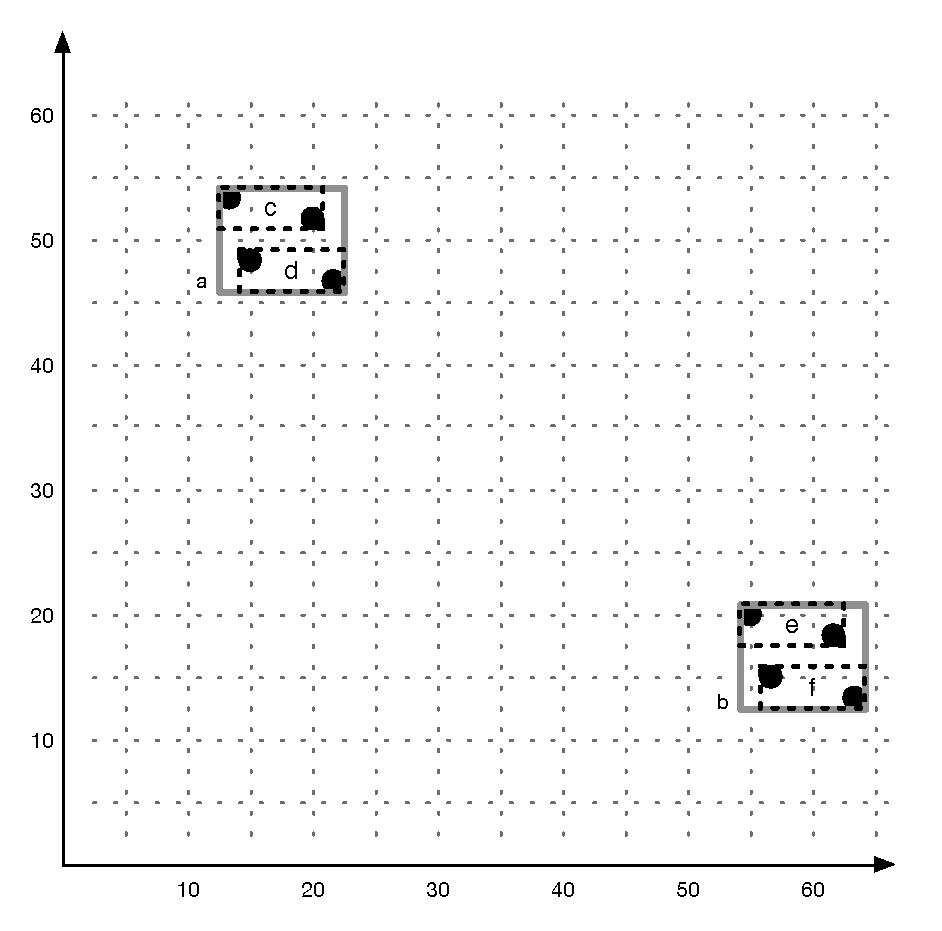
\includegraphics[width=0.4\textwidth]{chapters/papers/compressedrangesearching/r-comp}
	}\quad\quad\quad\quad\subfloat[R tree.]{
		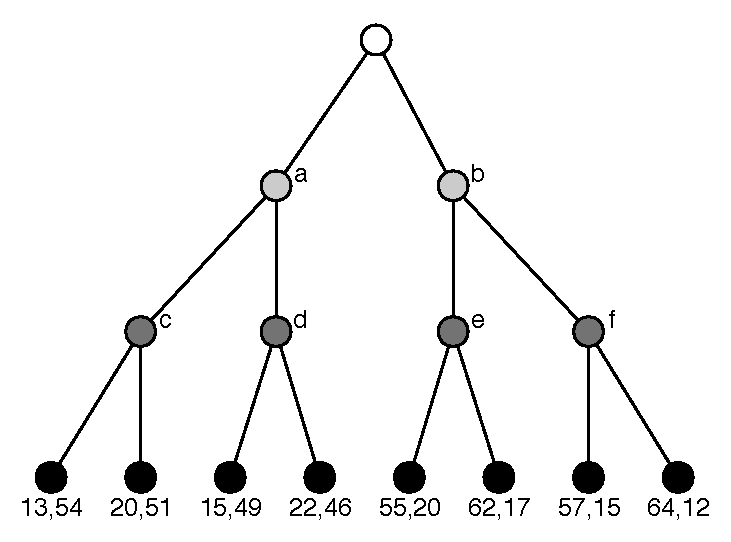
\includegraphics[width=0.4\textwidth]{chapters/papers/compressedrangesearching/rtree-comp}
	}
	\caption{A two-dimensional point set with R tree ranges overlaid, and the resulting R tree. Blue ranges are children of the root in the tree, red ranges are at the second level. A vertex label ($a$ - $h$) in the R tree identifies the range. We have omitted the precise coordinates for the ranges, but e.g. range $a$ spans the range $[13, 22] \times [46, 54]$ \label{fig:r-rep}}
	\end{center}
\end{figure} 

%%%%%%%%%%%%%%%%%%%%%%%%%%%%%%%%%%%%%%%%%%%%%%%%%%%%%%%%%%%%%%%%%%
%%%%%%%%%%%%%%%%%%% ABSOLUTE RANGE TREE TO DAG %%%%%%%%%%%%%%%%%%%
%%%%%%%%%%%%%%%%%%%%%%%%%%%%%%%%%%%%%%%%%%%%%%%%%%%%%%%%%%%%%%%%%%
\section{Compressed Canonical Range Searching}\label{sec:compcrs}
We now show how to compress geometric repetitions in any canonical range searching data structure $T$ while incurring only a constant factor overhead in queries. To do so we convert $T$ into a \emph{relative tree} representation, which we then compress into a minimal DAG representation that replaces geometric repetitions by single occurrences. We then show how to simulate a range query on $T$ with only constant overhead directly on the compressed representation. Finally, we extend the result to the I/O model of computation.

\subsection{The Relative Tree}
A \emph{relative tree} $R$ is an ordered, rooted and labeled tree storing a relative representation of a canonical range searching data structure $T$. The key idea is we can encode a range or a point $r = [ x_1, x'_1 ] \times \ldots \times [ x_k, x'_k ]$ as two $k$-dimensional vectors $\position(r) = (x_1, \ldots, x_k)$ and $\rangespan(r) = (x'_1 - x_1, \ldots, x'_k - x'_k)$ corresponding to an \emph{origin position} and an \emph{extent} of $r$. We use this representation in the relative tree, but only store extent vectors at vertices explicitly. The origin position vector for the range $\range{v}$ of a vertex $v \in R$ is calculated from offset vectors stored on the path from the root of $R$ to $v$, denoted $\rootpath(v)$. 

Formally, each vertex $v \in R$ stores a label, $\vlabel(v)$, and a $k$-dimensional extent vector $\rangespan(\range{v})$. Furthermore, each edge $(u, v) \in R$ stores an offset vector $\offset(u, v)$. The position vector for $\range{v}$ is calculated as $\position(\range{v}) = \sum_{(a, b) \in \rootpath(v)} \offset(a, b)$.
We say that two vertices $v, w \in R$ are \emph{equivalent} if the subtrees rooted at the vertices are isomorphic, including all labels and vectors. That is, $v$ and $w$ are equivalent if the two subtrees $R(v)$ and $R(w)$ are equal. 

It is straightforward to convert a canonical range searching data structure into the corresponding relative tree.
\begin{lemma}\label{lem:abs2rel}
Given any canonical range searching data structure $T$, we can construct the corresponding relative tree $R$ in linear time and space. 
\end{lemma}
\begin{proof}
First, note that a relative tree allows each vertex to store extent vectors and labels. Thus, to construct a relative tree $R$ representing the canonical range searching data structure $T$, we can simply copy the entire tree including extent vectors and vertex labels. So we only need to show how to store offset vectors in $R$ to ensure that the ranges for each pair of copied vertices are equal.

Consider a vertex $v \in T$ and its copy $v_R \in R$ and their parents $w \in T$ and $w_R \in R$. Since the extent vector and vertex labels are copied, $\rangespan(\range{v}) = \rangespan(\range{v_R})$ and $\vlabel(v) = \vlabel(v_R)$. The offset vector for edge $(w_R, v_R)$ is $\offset(w_R, v_R) = \position(\range{v}) - \position(\range{w})$. We assume the offset for the root is the 0-vector. Observe that summing up all the offset vectors on $\rootpath(v)$ is exactly $\position(\range{v})$, and so $\position(\range{v_R}) = \position(\range{v})$.

Since each vertex and edge in $T$ is only visited a constant number of times during the mapping, the construction time for $R$ is $O(N)$. The total number of labels stored by $R$ is asymptotically equal to the number of labels stored by $T$. Finally, the degrees of vertices does not change from $T$ to $R$. Thus, if $v \in T$ is mapped to $v_R \in R$ and $v$ requires $s$ space, $v_R$ requires $\Theta(s)$ space.
\end{proof}

\subsection{The Data Structure}
The compressed canonical data structure is the minimal DAG $G$ of the relative tree $R$ for $T$. By Lemma~\ref{lem:abs2rel} and~\cite{downey1980variations} we can build it in $O(N)$ time. Since $G$ replaces equivalent subtrees in $R$ by a single subtree, geometric repetitions in $T$ are stored only once in $G$. For an example, see Figure~\ref{fig:r-compression}. 
\begin{figure}[tb]
	\begin{center}
	\subfloat[Relative tree.]{
		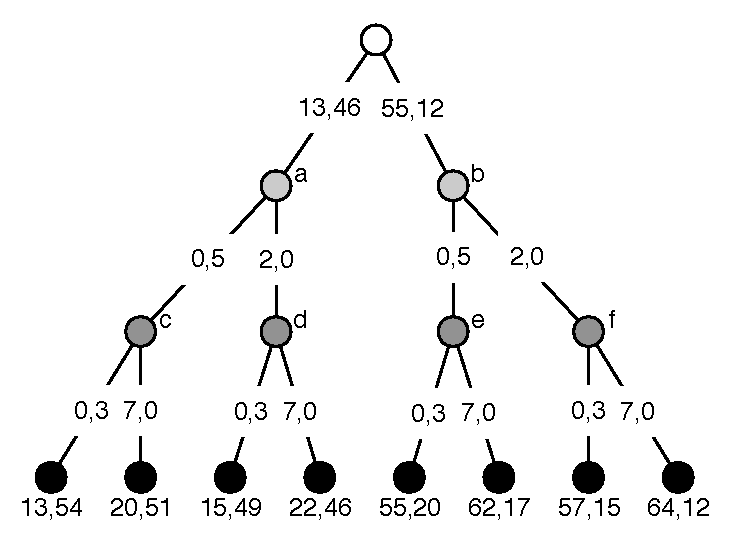
\includegraphics[width=0.4\textwidth]{chapters/papers/compressedrangesearching/rtree-relative}
	}\quad\quad\quad\quad\subfloat[Minimal DAG.]{
		\makebox[0.4\textwidth]{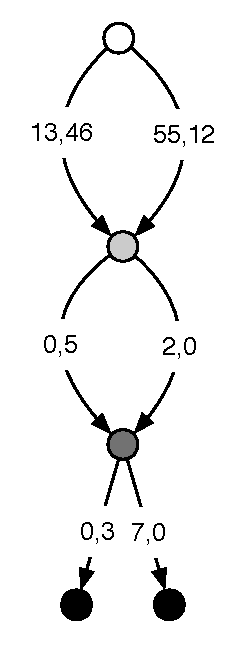
\includegraphics[height=0.3\textwidth]{chapters/papers/compressedrangesearching/rtree-dag}}
	}
	\caption{The relative tree obtained from the R tree from Figure \ref{fig:r-rep} and the resulting minimal DAG $G$ generating the tree. Only coordinates of the lower left corner of the ranges in the R tree are shown. In the relative tree, the absolute coordinates for the points are only shown for illustration, in order to see that the relative coordinates sum to the absolute coordinate along the root-to-leaf paths \label{fig:r-compression}}
	\end{center}
\end{figure}

Now consider a range query $Q$ on the canonical range searching data structure $T$. We show how to simulate $Q$ efficiently on $G$. Assuming $v_G \in G$ generates $v_R \in R$, we say that $v_G$ generates $v \in T$ if $v_R$ is the relative tree representation of $v$. When we visit a vertex $v_G \in G$, we calculate the origin position $\position(\range{v_G})$ from the sum of the offset vectors along the root-to-$v_G$ path. The origin position for each vertex can be stored on the way down in $G$, since we may only visit a vertex after visiting all ancestors (meaning that we can only arrive at $v_G$ from a root-to-$v_G$ path in $G$). Thus, it takes constant time to maintain the origin position for each visited vertex. Finally, a visit to a child of $v \in T$ can be simulated in constant additional time by visiting a child of $v_G \in G$. So we can simulate a visit to $v \in T$ by visiting the vertex $v_G \in G$ that generates $v$ and in constant time calculate the origin position for $v_G$. 

Any label comparison takes the same time on $G$ and $T$ since the label must be equal for $v_G \in G$ to generate $v \in T$. Now, since there is only constant overhead in visiting a vertex and comparing labels, it follows that if $Q$ uses $t$ time we can simulate it in $O(t)$ time on $G$. In summary, we have the following result.

\begin{theorem}\label{thm:compCan}
	Given a canonical range searching data structure $T$ with $N$ vertices, we can build the minimal DAG representation $G$ of $T$ in linear time. The space required by $G$ is $O(n)$, where $n$ is the size of the minimal DAG for a relative representation of $T$. We can support any query $Q$ on $T$ that takes time $t$ on $G$ in time $O(t)$. 
\end{theorem} 
As an immediate corollary, we get the following result for a number of concrete range searching data structures.
\begin{corollary}
	Given a K-D tree, Quad tree, R tree or Range tree, we can in linear time compress it into a data structure using space proportional to the size of the minimal relative DAG representation which supports canonical range searching queries with $O(1)$ overhead.
\end{corollary}


%%%%%%%%%%%%%%%%%%%%%%%%%%%%%%%%%%%%%%%%%%%%%%%%%%%%%%%%%%%%%%%%%%
%%%%%%%%%%%%%%%%%%%%%% I/O EFFICIENT QUERIES %%%%%%%%%%%%%%%%%%%%%
%%%%%%%%%%%%%%%%%%%%%%%%%%%%%%%%%%%%%%%%%%%%%%%%%%%%%%%%%%%%%%%%%%
\subsection{Extension to the I/O Model}
We now show that Theorem~\ref{thm:compCan} extends to the I/O model of computation. We assume that each vertex in $T$ require $\Theta(B)$ space, where $B$ is the size of a disk block. To allow for such vertices, we relax the definition of a canonical range searching data structure to allow it to store $B$ $k$-dimensional ranges. From Lemma~\ref{lem:abs2rel} and~\cite{downey1980variations}, if a vertex $v \in T$ require $\Theta(B)$ space, then so does the corresponding vertex $v_G \in G$. Thus, the layout of the vertices on disk does not asymptotically influence the number of disk reads necessary to answer a query, since only a constant number of vertices can be retrieved by each disk read. This means that visiting a vertex in either case takes a constant number of disk blocks, and so the compressed representation does not asymptotically increase the number of I/Os necessary to answer the query. Hence, we can support any query $Q$ that uses $p$ I/Os on $T$ using $O(p)$ I/Os on $G$. 


%%%%%%%%%%%%%%%%%%%%%%%%%%%%%%%%%%%%%%%%%%%%%%%%%%%%%%%%%%%%%%%%%%
%%%%%%%%%%%%%%%%%%%%% SIMILARITY CLUSTERING %%%%%%%%%%%%%%%%%%%%%%
%%%%%%%%%%%%%%%%%%%%%%%%%%%%%%%%%%%%%%%%%%%%%%%%%%%%%%%%%%%%%%%%%%
\section{Similarity Clustering}\label{sec:clustering}
We now introduce the \emph{similarity clustering} algorithm. Even if there are significant geometric repetitions in the point set $P$, the standard range searching data structures may not be able to capture this and may produce data structures that are not compressible. The similarity clustering algorithm allows us to create a canonical range searching data structure for which we can guarantee good compression using Theorem~\ref{thm:compCan}.

\subsection{Definitions}
\paragraph{Points and point sets}
We consider points in $k$-dimensional space, assuming $k$ is constant. The distance between two points $p_1$ and $p_2$, denoted $d(p_1, p_2)$, is their euclidian distance. We denote by $P = \{ p_1, p_2, \ldots, p_r \}$ a point set containing $r$ points. We say that two point sets $P_1, P_2$ are \emph{equivalent} if $P_2$ can be obtained from $P_1$ by translating all points with a constant $k$-dimensional offset vector.

The minimum distance between a point $p_q$ and a point set $P$ is the distance between $p_q$ and the closest point in $P$, $\mindist(P, p_q) = \min_{p \in P} d(p, p_q)$. The minimum distance between two point sets $P_1, P_2$ is the distance between the two closest points in the two sets, $\mindist(P_1, P_2) = \min_{p_1 \in P_1, p_2 \in P_2} d(p_1, p_2)$. These definitions extend to maximum distance in the natural way, denoted $\maxdist(P, p_q)$ and $\maxdist(P_1, P_2)$. The diameter of a point set $P$ is the maximum distance between any two points in $P$, $\diameter(P) = \max_{p_1, p_2 \in P} d(p_1, p_2) = \maxdist(P, P)$.

A point set $P_1 \subset P$ is \emph{lonely} if the distance from $P_1$ to any other point is more than twice $\diameter(P_1)$, i.e. $\mindist(P_1, P \setminus P_1) > 2 \times \diameter(P_1)$.

\paragraph{Clustering}
A hierarchical clustering of a point set $P$ is a tree, denoted $\clustering(P)$, containing the points in $P$ at the leaves. Each node in the tree $\clustering(P)$ is a cluster containing all the points in the leaves of its subtree. The root of $\clustering(P)$ is the cluster containing all points. We denote by $\points(v)$ the points in cluster node $v \in \clustering(P)$. Two cluster nodes $v, w \in \clustering(P)$ are equivalent if $\points(v)$ is equivalent to $\points(w)$ and if the subtrees rooted at the nodes are isomorphic such that each isomorphic pair of nodes are equivalent.

\subsection{Hierarchical Clustering Algorithm for Lonely Point Sets}
Order $P$ in lexicographically increasing order according to their coordinates in each dimension, and let $\Delta(P)$ denote the ordering of $P$.
The similarity clustering algorithm performs a greedy clustering of the points in $P$ in levels $i = 0, 1, \ldots, \log D+1$, where $D = \diameter(P)$. Each level $i$ has an associated clustering distance threshold $d_i$, defined as $d_0 = 0$ and $d_i = 2^{i-1}$ for all other $i$.

The clustering algorithm proceeds as follows, processing the points in order $\Delta(P)$ at each level. If a point $p$ is not clustered at level $i > 0$, create a new cluster $C_i$ centered around the point $p$ (and its cluster $C_{i-1}$ at the previous level). Include a cluster $C_{i-1}$ from level $i-1$ in $C_i$ if $\maxdist(\points(C_{i-1}), p) \leq d_i$. The clusters at level $0$ contain individual points and the cluster at level $\log D+1$ contains all points.

\begin{lemma}\label{lem:clustAlg}
	Given a set of points $P$, the similarity clustering algorithm produces a clustering tree containing equivalent clusters for any pair of equivalent lonely point sets.
\end{lemma}
\begin{proof}
Let $P_1$ and $P_2$ be two lonely point sets in $P$ such that $P_1$ and $P_2$ are equivalent, and let $d = \diameter(P_1) = \diameter(P_2)$. Observe that a cluster formed at level $i$ has at most diameter $2d_i = 2^i$. Thus, since all points are clustered at every level and all points outside $P_1$ have a distance greater than $2d$ to any point in $P_1$, there is a cluster $c \in \clustering(P)$ formed around point $a \in P_1$ at level $j = \lceil \log d \rceil$ containing no points outside $P_1$. Now, assume some point $p \in P_1$ is not in $\points(c)$. As all unclustered points within distance $2^j \geq d$ from $a$ are included in $c$, this would mean that $p$ was clustered prior to creating $c$. This contradicts the assumption that $P_1$ is lonely, since it can only happen if some point outside $P_1$ is closer than $2d$ to $p$. Concluding, $c$ contains exactly the points in $P_1$. The same argument naturally extends to $P_2$.

Now, let $C_1, C_2$ be the clusters containing the points from $P_1, P_2$, respectively. Observe that $\points(C_1)$ and $\points(C_2)$ are equivalent. Furthermore, because each newly created cluster process candidate clusters to include in the same order, the resulting trees for $C_1$ and $C_2$ are isomorphic and have the same ordering. Thus, the clusters $C_1$ and $C_2$ are equivalent.
\end{proof}

Because the clustering proceeds in $O(\log D)$ levels, the height of the clustering tree is $O(\log D)$. Furthermore, by considering all points and all of their candidates at each level, the clustering can be implemented in time $O(N^2 \log D)$. Observe that the algorithm allows creation of paths of clusters with only a single child cluster. If such paths are contracted to a single node to reduce the space usage, the space required is $O(N)$ words. In summary, we have the following result. 

\begin{theorem}\label{thm:clustering}
	Given a set of $N$ points with diameter $D$, the similarity clustering algorithm can in $O(N^2 \log D)$ time create a tree representing the clustering of height $O(\log D)$ requiring $O(N)$ words of space. The algorithm guarantees that any pair of equivalent lonely point sets results in the same clustering, producing equivalent subtrees in the tree representing the clustering.
\end{theorem}

Since the algorithm produces equivalent subtrees in the tree for equivalent lonely point sets, the theorem gives a compressible canonical range searching data structure for point sets with many geometric repetitions.


\section{Open Problems}
The technique described in this paper for generating the relative tree edge labels only allows for translation of the point sets in the underlying subtrees. However, the given searching technique and data structure generalizes to scaling and rotation (if simply storing a parent-relative scaling factor and rotation angle in each node, along with the nodes parent-relative translation vector). We consider it an open problem to efficiently construct a relative tree that uses such transformations of the point set. 

Another interesting research direction is if it is possible to allow for small amounts of noise in the point sets. That is, can we represent point sets that are almost equal (where few points have been moved a little) in a compressed way? An even more general question is how well one can do when it comes to compression of higher dimensional data in general.

Finally, the $O(N^2 \log D)$ time bound for generating the similarity clustering is prohibitive for large point sets. So an improved construction would greatly benefit the possible applications of the clustering method and is of great interest.

%\bibliographystyle{splncs03}

%\nocite{*}
%\bibliography{references}

%\end{document}
 %geometry, compression, ds
    %!TEX root = ../../../Thesis.tex
\chapter{Colored Range Searching in Linear Space}\label{chp:coloredrangesearching}

\begin{infosection}
    \begin{authors}
        Roberto Grossi\uni{1}\footnote{Partially supported by Italian MIUR PRIN project AMANDA.} \qquad S{\o}ren Vind\uni{2}\footnote{Supported by a grant from the Danish National Advanced Technology Foundation.}
    \end{authors}

    \begin{uninames}
        \uni{1} Universit\`{a} di Pisa \\
        \uni{2} Technical University of Denmark
    \end{uninames}

    \begin{abstract}
    In \emph{colored range searching}, we are given a set of $n$ colored points in $d \geq 2$ dimensions to store, and want to support orthogonal range queries taking colors into account. In the \emph{colored range counting} problem, a query must report the number of distinct colors found in the query range, while an answer to the \emph{colored range reporting} problem must report the distinct colors in the query range.
    
    We give the first linear space data structure for both problems in two dimensions ($d=2$) with $o(n)$ worst case query time. We also give the first data structure obtaining almost-linear space usage and $o(n)$ worst case query time for points in $d > 2$ dimensions. Finally, we present the first dynamic solution to both counting and reporting with $o(n)$ query time for $d \geq 2$ and $d \geq 3$ dimensions, respectively.
    \end{abstract}
\end{infosection}

%%%%%%%%%%%%%%%%%%%%%%%%%%%%%%%%%%%%%%%%%%%%%%%%%%%%%%%%%%%%%%%%%%
%%%%%%%%%%%%%%%%%%%%%%%%%% INTRODUCTION %%%%%%%%%%%%%%%%%%%%%%%%%%
%%%%%%%%%%%%%%%%%%%%%%%%%%%%%%%%%%%%%%%%%%%%%%%%%%%%%%%%%%%%%%%%%%
\section{Introduction}
\label{sec:crc-introduction}
%
In standard range searching a set of points must be stored to support queries for any given orthogonal $d$-dimensional query box $Q$ (see \cite{de2008orthogonal} for an overview). Two of the classic problems are standard range reporting, asking for the points in $Q$, and standard range counting, asking for the number of points in $Q$. In 1993, Janardan and Lopez \cite{janardan1993generalized} introduced one natural generalisation of standard range searching, requiring each point to have a color. This variation is known as \emph{colored range searching}\footnote{Also known in the literature as \emph{categorical} or \emph{generalized} range searching.}. 
The two most studied colored problems are \emph{colored range reporting}, where a query answer must list the distinct colors in $Q$, and \emph{colored range counting}, where the number of distinct colors in $Q$ must be reported. 

As shown in Tables~\ref{tab:count}--\ref{tab:report}, there has been a renewed interest for these problems due to their applications. For example, in database analysis and information retrieval the $d$-dimensional points represent entities and the colors are \emph{classes} (or categories) of entities. Due to the large amount of entities, statistics about their classes is the way modern data processing is performed.  A colored range query works in this scenario and reports some \emph{statistical analysis} for the classes using the range on the entities as a filtering method: ``which kinds of university degrees do European workers with age between 30 and 40 years and salary between 30,000 and 50,000 euros have?''. Here the university degrees are the colors and the filter is specified by the range of workers that are European with the given age and salary. The large amount of entities involved in such applications calls for nearly \emph{linear space} data structures, which is the focus of this paper.

\begin{table}[t]
    \centering
    \begin{tabular}{c c c c c}
       %\hline
    Dim. & Query Time               & Space Usage                          & Dyn. & Ref.    \\[1mm]
        \hline\\[-3mm]
    $1$        & $O(\log n / \log \log n)$& $O(n)$                             & $\times$ & $\mathsection$ \\[1mm]
    \hline\\[-3mm]
%%    $d=2$        & $O(n)$                   & $O(n)$ &  \\
            & $O(\log^2 n)$            & $O(n^2 \log^2 n)$                    & & $\star$  \\
            & $O(\log^2 n)$            & $O(n^2 \log^2 n)$                    & & $\dagger$ \\
    $2$   & $O(X \log^7 n)$          & $O((\frac{n}{X})^2 \log^6 n + n \log^4 n)$ & & $\dagger$ \\
            & $O\left( ( \frac{\sigma}{\log n} + \frac{n}{\log ^c n} ) (\log \log ^c n)^{2+\epsilon} \right)$ & $O(n)$ & & New \\[1mm]
    \hline\\[-3mm]
            & $O(\log^{2(d-1)} n)$     & $O(n^d \log ^{2(d-1)} n)$            & & $\dagger$ \\
    $> 2$  & $O(X \log^{d-1} n)$      & $O((\frac{n}{X})^{2d} + n \log^{d-1} n)$   & & $\dagger$ \\
            & $O\left(( \frac{\sigma}{\log n} + \frac{n}{\log ^c n} ) (\log  \log^{c} n)^{d-1} \log \log \log ^c n\right)$ & $O\!\left(n (\log \log^{c} n)^{d-1} \right)$ & & New \\[1mm]
     \hline\\[-3mm]
    $\geq 2$  & $O\left( ( \frac{\sigma}{\log n} + \frac{n}{\log ^c n} ) (\log \log ^c n)^{d} \right)$ & $O\!\left(n (\log \log^{c} n)^{d-1} \right)$ & $\times$ & New \\[1mm]
        \hline\\[-3mm]
    \end{tabular}
    \caption{Known and new solutions to \emph{colored range counting}, ordered according to decreasing space use in each dimension group. Dyn. column shows if solution is dynamic, $d$ is the dimensionality. References are abbreviated $\mathsection$ = \cite{jaja2005space}, $\star$ = \cite{gupta1995further}, $\dagger$ = \cite{kaplan2007counting}}
 \label{tab:count}
\end{table}


Curiously, counting is considered harder than reporting among the colored range queries as it is not a decomposable problem: knowing the number of colors in two halves of $Q$ does not give the query answer. This is opposed to reporting where the query answer can be obtained by merging the list of colors in two halves of $Q$ and removing duplicates. For the standard problems, both types of queries are decomposable and solutions to counting are generally most efficient.

In the following, we denote the set of $d$-dimensional points by $P$ and let $n = |P|$. The set of distinct colors is $\Sigma$ and  $\sigma = |\Sigma| \leq n$, with $k \leq \sigma$ being the number of colors in the output. We use the notation $\log^a b = (\log b)^a$ and adopt the RAM with word size $w = \Theta(\log n)$ bits, and the size of a data structure is the number of occupied words. 

Observe that for both colored problems, the trivial solution takes linear time and space, storing the points and looking through all of them  to answer the query. Another standard solution is to store one data structure for all points of each color that supports standard range emptiness queries (``is there any point inside $Q$?''). In two dimensions, this approach can answer queries in $O(\sigma \log n)$ time and linear space using a range emptiness data structure by Nekrich \cite{nekrich2009orthogonal}.
%However, this may be worse than the trivial solution, depending on $\sigma$.
However, since $\sigma = n$ in the worst case, this does not guarantee a query time better than trivial. 
Due to the extensive history and the number of problems considered, we will present our results before reviewing existing work.
%

\begin{table}[ht]
    \centering
    \begin{tabular}{c c c c c}
    %\hline
    Dim. & Query Time               & Space Usage                          & Dyn. & Ref.     \\[1mm]
    \hline\\[-3mm]
    $1$        & $O(1+k)$         & $O(n)$              & $\times$ & $\mathsection$             \\[1mm]
    \hline\\[-3mm]
                 & $O(\log n+k)$    & $O(n \log n)$       & & $\dagger$                 \\
    $2$        & $O(\log^2 n+k\log n)$    & $O(n \log n)$       & $\times$ & $\star$, $\ddagger$  \\
%    $d=2$        & $O(n)$                   & $O(n)$ & Naive \\
                & $O\left( ( \frac{\sigma}{\log n} + \frac{n}{\log ^c n} ) (\log\log^c n)^{2+\epsilon}  + k\right)$ & $O(n)$  & & New \\[1mm]
     \hline\\[-3mm]
    $\geq 2$  & $O\left( ( \frac{\sigma}{\log n} + \frac{n}{\log ^c n} ) (\log \log ^c n)^{d} + k\right)$ & $O\!\left(n (\log \log^{c} n)^{d-1} \right)$ & $\times$ & New \\[1mm]
    \hline\\[-3mm]
    $3$        & $O(\log ^2 n+k)$ & $O(n \log^4 n)$     & & $\star$               \\
    $> 3$      & $O(\log n+k)$    & $O(n^{1+\epsilon})$ & & $\diamond$, $\$$ \\ 
    $\geq 3$        & $O\left(( \frac{\sigma}{\log n} + \frac{n}{\log^c n} ) (\log\log^c n)^{d-1} \log \log \log^c n + k\right)$ & $O\!\left(n (\log\log^c n)^{d-1}\right)$ & & New \\[1mm]
\hline\\[-3mm]
    \end{tabular}
    \caption{Known and new solutions to \emph{colored range reporting}, ordered according to decreasing space use in each dimension group. Dyn. column shows if solution is dynamic, $d$ is the dimensionality. References are abbreviated $\mathsection$ = \cite{nekrich2013optimal}, $\star$ = \cite{gupta1995further}, $\dagger$ = \cite{shi2005optimal}, $\ddagger$ = \cite{bozanis1995new}, $\diamond$ = \cite{van1992new}, $\$$ = \cite{gupta1997technique}}
    \label{tab:report}
\end{table}


\subsection{Our Results}
\label{sub:our-results}
%
We observe (see Section~\ref{sub:previous-results}) that there are no known solutions to any of the colored problems in two dimensions that uses $O(n)$ words of space and answer queries in $o(n)$ worst case time. Furthermore, for colored range reporting there are no known solutions in $d> 3$ dimensions using $o(n^{1+\epsilon})$ words of space and answering queries in $o(n)$ worst case time. For colored range counting, no solutions with $o(n \polylog n)$ words of space and $o(n)$ worst case time exist. 

We present the first data structures for colored range searching achieving these bounds, improving almost logarithmically over previously known solutions in the worst case (see Section~\ref{sub:previous-results} and Tables~\ref{tab:count}--\ref{tab:report}). Specifically, we obtain
\begin{itemize}
    \item $o(n)$ query time and $O(n)$ space in two dimensions,
    \item $o(n)$ query time and $o(n \polylog n)$ space for counting in $d \geq 2$ dimensions,
    \item $o(n)$ query time and $o(n^{1+\epsilon})$ space for reporting in $d > 3$ dimensions,
    \item $o(n)$ query time supporting $O(\mathrm{polylg \,} n)$ updates in $d \geq 2$ and $d \geq 3$ dimensions for counting and reporting, respectively.
\end{itemize}

%The results improve almost logarithmically over the query time of previously known solutions in linear space in the worst case. 

We note that while our bounds have an exponential dimensionality dependency (as most previous results), it only applies to $\log \log n$ factors in the bounds.
Our solutions can be easily implemented and parallelized, so they are well-suited for the distributed processing of large scale data sets. Our main results can be summarised in the following theorems, noting that $c > 1$ is an arbitrarily chosen integer, and $\sigma \leq n$ is the number of distinct colors.

%%% Two dimensions:
\begin{theorem}\label{thm:2D}
    There is a linear space data structure for two-dimensional colored range counting and reporting storing $n$ points, each assigned one of $\sigma$ colors. The data structure answers queries in time $O( ( \sigma / \log n + n / \log ^c n ) (\log \log ^c n)^{2+\epsilon} )$, with reporting requiring an additive term $O(k)$.
\end{theorem}

%%% Many dimensions:
\begin{theorem}\label{thm:dD}
  There is a $O(n (\log \log ^{c} n) ^{d-1})$ space data structure storing $n$ $d$-dimensional colored points each assigned one of $\sigma$ colors. Each colored range counting and reporting query takes time $O(( \sigma / \log n + n / \log ^c n ) (\log \log ^{c} n) ^{d-1} \log \log \log ^c n )$. Reporting requires an additive $O(k)$ time.
\end{theorem}

To obtain these results, we partition points into groups depending on their color. Each group stores all the points for at most $\log n$ specific colors. Because the colors are partitioned across the groups, we can obtain the final result to a query by merging query results for each group (and we have thus obtained a decomposition of the problem along the color dimension). A similar approach was previously used in \cite{kaplan2007counting}.

In order to reduce the space usage of our data structure, we partition the points in each group into a number of buckets of at most $\log^c n$ points each. The number of buckets is $O(\sigma / \log n + n / \log ^c n)$, with the first term counting all underfull buckets and the second counting all full buckets. Each bucket stores $m \leq \log ^c n$ points colored with $f \leq \log n$ different colors.
%Our approach partitions points into groups depending on their color. Each group stores all points of $\leq \log n$ specific colors. A further subdivision of the groups into buckets ensures that the number of points in each bucket is $O(\log ^c n)$. Thus, the number of buckets is $O(\sigma / \log n + n / \log ^c n)$ (the first term counts all underfull buckets, the second counts all full buckets). Because the colors are partitioned across the groups, we can obtain the final result to a query by summing the number of colors found in each group (and we have thus obtained a decomposition of the problem along the color dimension). 
%As the colors of each group may be present in several buckets, we cannot obtain the solution for a group from an individual count for each bucket (since we risk counting a color several times). 
%Instead, we use an efficient solution to the $d$-dimensional \emph{colored range reporting problem} in the buckets (where the number of points is $m \leq \log ^c n$ and the number of colors is $f \leq \log n$). 
To avoid counting a color several times across different buckets, we use a solution to the $d$-dimensional colored range reporting problem in each bucket for which answers to queries are given as bitstrings. Answers to the queries in buckets can be merged efficiently using bitwise operations on words.
%and require that the answer to a query is given as a $f$-bit long bitstring. Since $f \leq w$, we can use bitwise OR operations to efficiently compose the answers to each of the queries on the buckets to produce the full answer for the group. 
We finally use an $o(n)$ space lookup table to obtain the count or list of colors present in the merged answer. 
%This takes constant time per answer found in the lookup table.

The solution to $d$-dimensional colored range reporting for each bucket is obtained by building a $d$-dimensional range tree for the $m$ points, which uses a new linear space and $O(\log \log m)$ time solution to restricted one-dimensional colored range reporting as the last auxiliary data structure. In total, each bucket requires $O(m \log ^{d-1} m)$ space and $O(\log ^{d-1} m \log \log m)$ query time. In two dimensions, we reduce the space to linear by only storing representative rectangles in the range tree covering $O(\log m)$ points each. Using the linear space range reporting data structure by Nekrich \cite{nekrich2009orthogonal}, we enumerate and check the underlying points for each of the $O(\log m)$ range tree leaves intersecting the query range, costing us a small penalty of $O(\log ^{\epsilon} n)$ per point. We thus obtain a query time of $O(\log ^{2+\epsilon} m)$ for two-dimensional buckets in linear space.

% Though the basic approach is simple, it allows us to give in Theorem % \ref{thm:2D} the first linear space data structure with $o(n)$ worst % case query time for two-dimensional colored range counting and colored % range reporting. Furthermore, Theorem \ref{thm:dD} is the first % almost-linear space data structure for both colored range counting and % colored range reporting in higher dimensions with $o(n)$ worst case % query time. 
% \fxfatal{Comparison needs to be improved.}

\vspace{0.5em}
Using classic results on dynamisation of range trees, we can dynamise the data structure with a little additional cost in query time. Previously, there was no known dynamic data structures with $o(n)$ query time for colored range counting in $d \geq 2$ dimensions and colored range reporting in $d \geq 3$ dimensions. Consequently, this is the first such dynamic data structure.

%%% Dynamic:
\begin{theorem}\label{thm:dyn-dD}
    There is a dynamic $O(n (\log \log ^{c} n) ^{d-1})$ space data structure storing $n$ $d$-dimensional colored points each assigned one of $\sigma$ colors. The data structure answers colored range counting and reporting queries in time $O(( \sigma / \log n + n / \log ^c n ) (\log \log ^{c} n) ^{d})$. Reporting requires a additive $O(k)$ time and updates are supported in $O((\log \log ^c n) ^d)$ amortised time.
\end{theorem}

Finally, if paying a little extra space, we can get a solution to the problem where the query time is bounded by the number of distinct colors instead of the number of points. This is simply done by not splitting color groups into buckets, giving the following result. 

%%% Colors
\begin{corollary}\label{thm:col-dD}
    There is a $O(n \log ^{d-1} n)$ space data structure for $n$ $d$-dimensional colored points each assigned one of $\sigma$ colors. The data structure answers colored range counting and reporting queries in time $O(\sigma \log ^{d-2} n \log \log n)$. Reporting requires a additive $O(k)$ time.
\end{corollary}

In two dimensions this is a logarithmic improvement over the solution where a range emptiness data structure is stored for each color at the expense of a $\log n$ factor additional space. The above approach can be combined with the range emptiness data structure by Nekrich \cite{nekrich2009orthogonal} to obtain an output-sensitive result where a penalty is paid per color reported:

%%% Colors, output-sensitive
\begin{corollary}\label{thm:col-2D}
    There is a $O(n \log n)$ space data structure storing $n$ two-dimensional colored points each assigned one of $\sigma$ colors. The data structure answers colored range counting and reporting queries in time $O(\sigma + k \log n \log \log n)$.
\end{corollary}

\subsection{Previous Results}
\label{sub:previous-results}
\paragraph*{Colored range counting.}
%
Colored range counting is challenging, with a large gap in the known bounds compared to standard range counting, especially in two or more dimensions. For example, a classic range tree solves two-dimensional standard range counting in logarithmic time and $O(n \log n)$ space, but no polylogarithmic time solutions in $o(n^2)$ space are known for colored range counting.

Larsen and van Walderveen \cite{larsen2013near, gupta1995further} showed that colored range counting in one dimension is equivalent to two-dimensional standard range counting. Thus, the optimal $O(\log n / \log \log n)$ upper bound for two-dimensional standard range counting by J{\'a}J{\'a} et al. \cite{jaja2005space} which matches a lower bound by Patrascu \cite{patrascu2007lower} is also optimal for one-dimensional colored range counting.

In two dimensions, Gupta et al. \cite{gupta1995further} show a solution using $O(n^2 \log^2 n)$ space that answers queries in $O(\log^2 n)$ time. They obtain their result by storing $n$ copies of a data structure which is capable of answering three-sided queries. The same bound was matched by Kaplan et al. \cite{kaplan2007counting} with a completely different approach in which they reduce the problem to standard orthogonal range counting in higher dimensions. Kaplan et al. also present a tradeoff solution with $O(X \log^7 n)$ query time and $O((\frac{n}{X})^2 \log^6 n + n \log^4 n)$ space for $1 \leq X \leq n$. Observe that the minimal space use for the tradeoff solution is $O(n \log^4 n)$.

In $d > 2$ dimensions, the only known non-trivial solutions are by Kaplan et al. \cite{kaplan2007counting}. One of their solutions answers queries in $O(\log ^{2(d-1)} n)$ time and $O(n^d \log ^{2(d-1)} n)$ space, and they also show a number of tradeoffs, the best one having $O(X \log^{d-1} n)$ query time and using $O((\frac{n}{X})^{2d} + n \log^{d-1} n)$ space for $1 \leq X \leq n$. In this case, the minimal space required by the tradeoff is $O(n \log ^{d-1} n)$.

Kaplan et al. \cite{kaplan2007counting} showed that answering $n$ two dimensional colored range counting queries in $O(n^{p/2})$ time (including all preprocessing time) yields an $O(n^p)$ time algorithm for multiplying two $n \times n$ matrices. For $p < 2.373$, this would improve the best known upper bound for matrix multiplication \cite{williams2012multiplying}. Thus, solving two dimensional colored range counting in polylogarithmic time per query and $O(n \polylog n)$ space would be a major breakthrough. This suggest that even in two dimensions, no polylogarithmic time solution may exist.

%Finally, Lai et al. presented a randomised approximate solution to colored range counting in $d$ dimensions, answering queries in time $O(d \log^{d+1} n)$ and space $O(dn \log ^{d-1} n)$ \cite{lai2005approximate,lai2008approximate}. Their data structure is randomized in the sense that the answer is expected to be correct to within a constant factor of the correct answer. 
%\fxfatal{SV: Removed approximate thing, as it does not really fit into anything. Check if you agree.}
% RG: removed  $\epsilon$  as we use for another purpose


\paragraph*{Colored range reporting.}
%
The colored range reporting problem is well-studied \cite{janardan1993generalized, nekrich2012space, nekrich2013optimal, nekrich2014efficient, gagie2012colored, shi2005optimal, gupta1995further, gupta1997technique, van1992new, mortensen2003generalized, bozanis1995new, larsen2012efficient}, with output-sensitive solutions almost matching the time and space bounds obtained for standard range reporting in one and two dimensions. In particular, Nekrich and Vitter recently gave a dynamic solution to one dimensional colored range reporting with optimal query time $O(1+k)$ and linear space \cite{nekrich2013optimal}, while Gagie et al. earlier presented a succinct solution with query time logarithmic in the length of the query interval \cite{gagie2012colored}.

In two dimensions, Shi and JaJa obtain a bound of $O(\log n + k)$ time and $O(n \log n)$ space \cite{shi2005optimal} by querying an efficient static data structure for three-sided queries, storing each point $O(\log n)$ times. Solutions for the dynamic two-dimensional case were developed in \cite{gupta1995further, bozanis1995new}, answering queries with a logarithmic penalty per answer. If the points are located on an $N \times N$ grid, Agarwal et al. \cite{agarwal2002range} present a solution with query time $O(\log \log N + k)$ and space use $O(n \log ^2 N)$. Gupta et al. achieve a static data structure using $O(n \log ^4 n)$ space and answering queries in $O(\log ^2 n + k)$ \cite{gupta1995further} in the three-dimensional case. To the best of our knowledge, the only known non-trivial data structures for $d> 3$ dimensions are by van Kreveld and Gupta et al., answering queries in $O(\log n + k)$ time and using $O(n^{1+\epsilon})$ space \cite{van1992new, gupta1997technique}. Other recent work on the problem include external memory model solutions when the points lie on a grid \cite{nekrich2012space, larsen2012efficient, nekrich2014efficient}.

% The paper is structured with Section \ref{sec:basics} giving the basic % approach using grouping and bucketing and reducing the problem to % restricted colored range reporting, proving Theorem \ref{thm:dD}. % Section \ref{sec:linear} proves Theorem \ref{thm:2D}, showing how to % reduce the space to linear in two dimensions. Section % \ref{sec:dynamic} shows how to dynamise the data structure and gives % Theorem \ref{thm:dyn-dD}, and Section \ref{sec:colors} show how to % obtain the color and output-sensitive bounds of Corollaries % \ref{thm:col-dD} and \ref{thm:col-2D}.


\section{Colored Range Searching in Almost-Linear Space}
\label{sec:basics}
%
We present here the basic approach that is modified to obtain our theorems. We first show how to partition the points into $O(\sigma / \log n + n / \log ^c n)$ buckets each storing $m = O(\log ^c n)$ points of $f = O(\log n)$ distinct colors, for which the results can be easily combined. We then show how to answer queries in each bucket in time $O(\log ^{d-1} m \log \log m)$ and space $O(m \log ^{d-1} m)$, thus obtaining Theorem \ref{thm:dD}.

\subsection{Color Grouping and Bucketing}
%
We partition the points of $P$ into a number of groups $P_i$, where $i = 1, \ldots, \frac{\sigma}{\log n}$, depending on their color. Each group stores all points having $f = \log n$ distinct colors (except for the last group which may store points with less distinct colors). For each group $P_i$ we store an ordered color list $L_i$ of the $f$ colors in the group. That is, a group may contain $O(n)$ points but the points have at most $f$ distinct colors. Since colors are partitioned among groups, we can clearly answer a colored query by summing or merging the results to the same query in each group. 
%Observe that assuming a colored range counting query can be answered for each group, we can clearly answer a colored range counting query by adding the results for each group (since colors are partitioned among groups).

\begin{figure}[tb]
	\begin{center}
	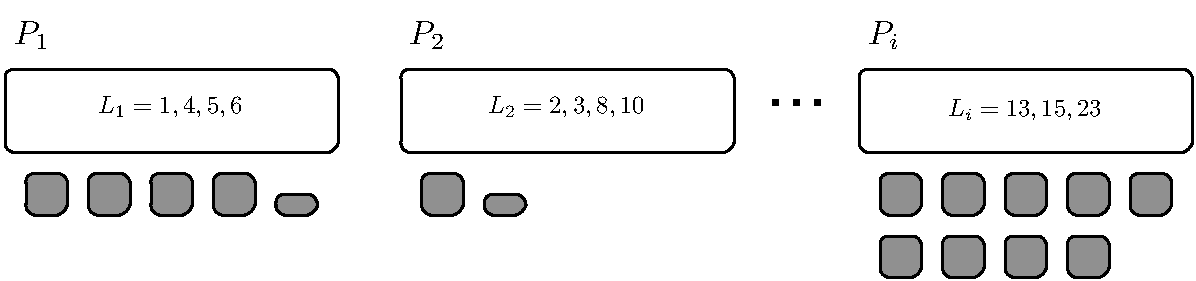
\includegraphics[width=0.9\textwidth]{chapters/papers/coloredrangecounting/groups-buckets}
	\caption{Grouping and bucketing of some point set with $f = 4$. The white boxes are the groups and the grey boxes below each group are buckets each storing $O(\log^c n)$ points\label{fig:groups-buckets}}
	\end{center}
\end{figure} 

Each group is further partitioned into a number of buckets containing $m = \log ^c n$ points each (except for the last bucket, which may contain fewer points). Since the buckets partition the points and there cannot be more than one bucket with fewer than $\log ^c n$ points in each group, the total number of buckets is $O(\sigma / \log n + n / \log ^c n)$. See Figure \ref{fig:groups-buckets} for an example of the grouping and bucketing. 

We require that each bucket in a group $P_i$ supports answering \emph{restricted colored range reporting queries} with an $f$-bit long bitstring, where the $j$th bit indicates if color $L_i[j]$ is present in the query area $Q$ in that bucket. Clearly, we can obtain the whole answer for $Q$ and $P_i$ by using bitwise OR operations to merge answers to the restricted colored range reporting query $Q$ for all buckets in $P_i$. We call the resulting bitstring $F_{i, Q}$, which indicates the colors present in the query range $Q$ across the entire group $P_i$.
%Clearly, a constant number of bitwise OR operations per bucket is enough to produce a $f$-bit long bitstring from a single restricted colored range reporting query per bucket. We call this bitstring $F_{i, Q}$, and note that it indicates the colors present in the query range across the entire group $P_i$.

Finally, we store a lookup table $T$ of size $O(\sqrt{n} \log n) = o(n)$ for all possible bitstrings of length $\frac{f}{2}$. For each bitstring, the table stores the number of {\bitone}s present in the bitstring and the indices where the {\bitone}s are present. Using two table lookups in $T$ with the two halves of $F_{i, Q}$, we can obtain both the number of colors present in $P_i$ for $Q$, and their indices into $L_i$ in $O(1)$ time per index. 

Summarising, we can merge answers to the restricted colored range reporting queries in $O(1)$ time per bucket and obtain the full query results for each group $P_i$. Using a constant number of table lookups per group, we can count the number of colors present in $Q$. There is $O(1)$ additional cost per reported color.
%Summarising, we can combine answers from each bucket in a group and add the results for all groups in time linear in the number of buckets for a colored range counting query. Thus, the total time spent is bounded by the number of buckets present multiplied by the time taken to answer a restricted colored range reporting query in a bucket. Additionally, we can answer colored range reporting queries in the same time plus $O(1)$ time per reported color.

\subsection{Restricted Colored Range Reporting for Buckets}
\label{sec:RCRR}
%
Each bucket in a group $P_i$ stores up to $m = \log^c n$ points colored with up to $f = \log n$ distinct colors, and must support restricted colored range reporting queries, reporting the colors in  query range $Q$ using an $f$-bit long bitstring. A simple solution is to use a classic $d$-dimensional range tree $R$, augmented with an $f$-bit long bitstring for each node on the last level of $R$ (using the $L_i$ ordering of the $f$ colors). The colors within the range can thus be reported by taking the bitwise OR of all the bitstrings stored at the $O(\log^d m)$ summary nodes of $R$ spanning the range in the last level. This solution takes total time $O(\frac{f}{w} \log ^d m) = O(\log ^d m)$ and space $O(m \log ^{d-1} m \frac{f}{w}) = O(m \log ^{d-1} m)$, and it can be constructed in time $O(m \log ^{d-1} m)$ by building the node bitstrings from the leaves and up (recall that $w = \Theta(\log n)$ is the word size). 

The above solution is enough to obtain some of our results, but we can improve it by replacing the last level in $R$ with a new data structure for restricted one-dimensional colored range reporting over integers that answer queries in time $O(\log \log m)$ and linear space. A query may perform $O(\log ^{d-1} m)$ one-dimensional queries on the last level of the range tree, so the query time is reduced to $O(\log ^{d-1} m \log \log m)$ per bucket. The new data structure used at the last level is given in the next section.

Observe that though the points are not from a bounded universe, we can remap a query in a bucket to a bounded universe of size $m$ in time $O(\log m)$ and linear space per dimension. We do so for the final dimension, noting that we only need to do it once for all $O(\log ^{d-1} m)$ queries in the final dimension. 

\subsubsection*{1D restricted colored range reporting on integers.}
%
Given $O(m)$ points in one dimension from a universe of size $m$, each colored with one of $f = \log n$ distinct colors, we now show how to report the colors contained in a query range in $O(\log \log m)$ time and linear space, encoded as an $f$-bit long bitstring. First, partition the points into $j = O(m / \log m)$ intervals spanning $\Theta(\log m)$ consecutive points each. Each interval is stored as a balanced binary search tree of height $O(\log \log m)$, with each node storing a $f$-bit long bitstring indicating the colors that are present in its subtree. Clearly, storing all these trees take linear space.

We call the first point stored in each interval a \emph{representative} and store a predecessor data structure containing all of the $O(m / \log m)$ representatives of the intervals. Also, each representative stores $O(\log m)$ $f$-bit long bitstrings, which are summaries of the colors kept in the $1, 2, \ldots, 2^{\log j}$ neighboring intervals. We store these bitstrings both towards the left and the right from the representative, in total linear space.


A query $[a, b]$ is answered as follows. 
We decompose the query into two parts, first finding the answer for all intervals fully contained in $[a, b]$, and then finding the answer for the two intervals that only intersect $[a, b]$. 
%We find two bitstrings summarising the answer for all intervals fully contained in $[a, b]$ and merge the result with bitstrings for the two intervals that intersect but are not fully contained in $[a, b]$. 
The first part is done by finding the two outermost representatives inside the interval (called $a', b'$, where $a \leq a' \leq b' \leq b$) by using predecessor queries with $a$ and $b$ on the representatives. 
%We first at most two bitstrings that are stored at the representatives and that cover the largest portion of $[a, b]$. This is equivalent to finding the two outermost intervals that are fully covered by $[a,b]$, which is done using predecessor/successor queries with $a$ and $b$ on the representatives. 
Since we store summaries for all power-of-2 neighboring intervals of the representatives, there are two bitstrings stored with $a'$ and $b'$ which summarises the colors in all fully contained intervals. 

To find the answer for the two intervals that contain $a$ or $b$, we find $O(\log \log m)$ nodes of the balanced binary tree for the interval and take the bitwise OR of the bitstrings stored at those nodes in $O(\log \log m)$ total time. Using one of the classic predecessor data structures \cite{van1976design, mehlhorn1990bounded, willard1983log} for the representatives, we thus obtain a query time of $O(\log \log m)$ and linear space.
%The colors found in the two intervals that contain $a$ and $b$ to obtain the final answer. That is, we find the bitstring answer for the two intervals $[a, a']$ and $[b', b]$ and merge these with the bitstring answers for interval $[a', b']$. The bitstring for $[a, a']$ or $[b', b]$ is determined by


\section{2D Colored Range Searching in Linear Space}
\label{sec:linear}
%
To obtain linear space in two dimensions and the proof of Theorem~\ref{thm:2D}, we use the same grouping and bucketing approach as in Section~\ref{sec:basics}. For each group $P_{i'}$, we only change the solution of each bucket $B_i$ in $P_{i'}$, recalling that $B_i$ contains up to $m = \log^c n$ points with $f = \log n$ distinct colors, so as to use linear space instead of $O(m \log m)$ words of space. 

We store a linear space 2D standard range reporting data structure $A_i$ due to Nekrich \cite{nekrich2009orthogonal} for all points in the bucket $B_i$. As shown in~\cite{nekrich2009orthogonal}, $A_i$ supports orthogonal standard range reporting queries in $O(\log m + r \log ^{\epsilon} m)$ time and updates in $O(\log ^{3+\epsilon} m)$ time, where $r$ is the reported number of points and $\epsilon > 0$.


% \begin{theorem}[Nekrich % \cite{nekrich2009orthogonal}]\label{thm:nekrich}
%     There is a linear space data structure storing $n$ two-dimensional % points which support orthogonal standard range reporting queries in % $O(\log n + k \log ^{\epsilon} n)$ time and updates in $O(\log % ^{3+\epsilon} n)$ time, where $k$ is the reported number of points and % $\epsilon > 0$.
% \end{theorem}

We also store a simple 2D range tree $R_i$ augmented with $f$-bit long bitstrings on the last level as previously described in Section~\ref{sec:RCRR}, but instead of storing points in $R_i$, we reduce its space usage by only storing areas covering $O(\log m)$ points of $B_i$ each. This can be done by first building $R_i$ taking $O(m \log m)$ space and time, and then cutting off subtrees at nodes at maximal height (called cutpoint nodes) such that at most $c' \log m$ points are covered by each cutpoint node, for a given constant $c'>0$. In this way, each cutpoint node is implicitly associated with $O(\log m)$ points, which can be succinctly represented with $O(1)$ words as they all belong to a distinct 2D range. Note that the parent of a cutpoint node has $\Omega(\log m)$ descending points, hence there are $O(m/\log m)$ cutpoint nodes.

A query is answered by finding $O(\log^2 m)$ summary nodes in $R_i$ that span the entire query range $Q$. Combining bitstrings as described in Section~\ref{sec:RCRR}, the colors for all fully contained ranges that are not stored in the leaves can thus be found. Consider now one such leaf $\ell$ covering an area intersecting $Q$: since the $O(\log m)$ points spanned by $\ell$ may not be all contained in $Q$, we must check those points individually. Recall that the points associated with $\ell$ are those spanning a certain range $Q'$, so they can be succinctly represented by $Q'$. To actually retrieve them, we issue a query $Q'$ to $A_i$, check which ones belong to $Q' \cap Q$, and build a bitstring for the colors in $Q' \cap Q$. We finally merge the bitstrings for all summary nodes and intersecting leaves in constant time per bitstring to obtain the final result.

The time spent answering a query is $O(\log ^2 m)$ to find all bitstrings in non-leaf nodes of $R_i$ and to combine all the bitstrings. The time spent finding the bitstring in leaves is $O(\log ^{1+\epsilon} m)$ per intersecting leaf as we use Nekrich's data structure $A_i$ with $r = O(\log m)$. Observe that only two leaves spanning a range of $O(\log m)$ points may be visited in each of the $O(\log m)$ second level data structures visited, so the time spent in all leaves is $O(\log ^{2+\epsilon} m)$, which is also the total time. Finally, since we reduced the size of the range tree by a factor $\Theta(\log m)$, the total space usage is linear. This concludes the proof of Theorem \ref{thm:2D}. 
%For higher dimension, we will show in the full version of the paper how to extend our approach using the data structure of Karpinski, Nekrich 2009.
%\fxfatal{Fix the reference}
% NOTE: I have not found any non-grid based $d>2$ and almost-linear space range reporting data structures. Thus left out.


% \begin{itemize}
%     \item Same approach can be used for higher dimensions (Karpinski, % Nekrich 2009): Not to linear space, but reducing space usage to $O(m % \log ^{d-2+\epsilon} m)$ per bucket.
%     \item In particular, in three dimensions, we can obtain a solution % with X space use and Y query time. \fxfatal{Probably not an % interesting note.}
% \end{itemize}

\section{Dynamic Data Structures}
\label{sec:dynamic}
%
We now prove Theorem~\ref{thm:dyn-dD} by discussing how to support operations $\opins(p, c)$ and $\opdel(p)$, inserting and deleting a point $p$ with color $c$, respectively. Note that the color $c$ may be previously unused. We still use parameters $f$ and $m$ to denote the number of colors in groups and points in buckets, respectively.
We first give bounds on how to update a bucket, and then show how to support updates in the color grouping and point bucketing. 

% We also give bounds when the buckets are implemented with the classic % range tree where each node on the final level is augmented with an % $f$-bit long bitstring over the colors in the subtree. 

\subsection{Updating a Bucket}
%
Updating a bucket with a point corresponds to updating a $d$-dimensional range tree using known techniques in dynamic data structures. Partial rebuilding \cite{andersson1999general, overmars1983design} requires amortised time $O(\log^d m)$, including updating the bitstrings in the partially rebuilt trees and in each node of the last level trees (which takes constant time). Specifically, the bitstrings for the $O(\log^{d-1} m)$ trees on the last level where a point was updated may need to have the bitstrings fixed on the path to the root on that level. This takes time $O(\log m)$ per tree, giving a total amortised update time of $O(\log^d m)$.

\subsection{Updating Color Grouping and Point Bucketing}
\label{sub:update-color-group-bucket}
%
When supporting $\opins(p, c)$, we first need to find the group to which $c$ belongs. If the color is new and there is a group $P_i$ with less than $f$ colors, we must update the color list $L_i$. Otherwise, we can create a new group $P_i$ for the new color. In the group $P_i$, we must find a bucket to put $p$ in. If possible, we put $p$ in a bucket with less than $m$ points, or otherwise we create a new bucket for $p$. Keeping track of sizes of groups and buckets can be done using priority queues in time $O(\log \log n)$. Note that we never split groups or buckets on insertions.

As for supporting $\opdel(p)$, we risk making both groups and buckets underfull, thus requiring a merge of either. A bucket is underfull when it contains less than $m/2$ points. We allow at most one underfull bucket in a group. If there are two underfull buckets in a group, we merge them in time $O(m \log^d m)$. Since merging buckets can only happen after $\Omega(m)$ deletions, the amortized time for a deletion in this case is $O(\log^d m)$. A group is underfull if it contains less than $f/2$ colors and, as for buckets, if there are any two underfull groups $P_i, P_j$, we merge them. When merging $P_i, P_j$ into a new group $P_r$, we concatenate their color lists $L_i, L_j$ into $L_r$, removing the colors that are no more present while keeping the relative ordering of the surviving colors from $L_i, L_j$. In this way, a group merge does not require us to merge the underlying buckets, as points are partitioned arbitrarily into the buckets. However, a drawback arises: as the color list $L_r$ for the merged group is different from the color lists $L_i, L_j$ used for answering bucket queries, this may introduce errors in bucket query answers. Recall that an answer to a bucket query is an $f$-bit long bitstring which marks with {\bitone}s the colors in $L_i$ that are in the range $Q$. So we have a bitstring for $L_i$, and one for $L_j$, for the buckets previously belonging to $P_i, P_j$, but we should instead output a bitstring for $L_r$ in time proportional to the number of buckets in $P_r$. We handle this situation efficiently as discussed in Section~\ref{sub:fixing-bucket-answers}.

\subsection{Fixing Bucket Answers During a Query}
\label{sub:fixing-bucket-answers}
%
As mentioned in Section~\ref{sub:update-color-group-bucket}, we do not change the buckets when two or more groups are merged into $P_r$. Consider the $f$-bit long bitstring $b_i$ that is the answer for one merged group, say $P'_i$, relative to its color list, say $L_i$. However, after the merge, only a sublist $L'_i \subseteq L_i$ of colors survives as a portion of the color list $L_r$ for $P_r$. We show how to use $L_i$ and $L'_i$ to contribute to the $f$-bit long bitstring $a$ that is the answer to query $Q$ for the color list $L_r$ in $P_r$. The time constraint is that we can spend time proportional to the number, say $g$, of buckets in $P_r$. 


% Observe that when merging two groups, at least $f/2$ of the bits in % any answer to a restricted colored range reporting in the buckets % belonging to the groups must be \bitzero. 


We need some additional information. For each merged group $P'_i$, we create an $f$-bit long bitstring $v_i$ with bit $j$ set to \bitone\ if and only if color $L_i[j]$ survives in $L_r$ (i.e. some point in $P_r$ has color $L_i[j]$). We call $v_i$ the \emph{possible answer bitstring} and let $o_i$ be the number of {\bitone}s in $v_i$: in other words, $L'_i$ is the sublist built from $L_i$ by choosing the colors $L_i[j]$ such that $v_i[j] = \bitone$, and $o_i = |L'_i|$. 

Consider now the current group $P_r$ that is the outcome of $h \leq f$ old merged groups, say $P'_1, P'_2, \ldots, P'_h$ in the order of the concatenation of their color lists, namely, $L_r = L'_1 \cdot L'_2 \cdots L'_h$.  Since the number of buckets in $P_r$ is $g \geq h$, we can spend $O(g)$ time to obtain the $f$-bit long bitstrings $b_1, b_2, \ldots, b_h$, which are the answers for the old merged groups $P'_1, P'_2, \ldots, P'_h$, and combine them to obtain the answer $a$ for $P_r$. 

Here is how. The idea is that the bits in $a$ from position $1+\sum_{l=1}^{i-1} o_l$ to $\sum_{l=1}^i o_l$ are reserved for the colors in $L'_i$, using \bitone\ to indicate which color in $L'_i$ is in the query $Q$ and \bitzero\ which is not. Let us call $b'_i$ this $o_i$-bit long bitstring. Recall that we have $b_i$, which is the $f$-bit long bitstring that is the answer for $P'_i$ and refers to $L_i$, and also $v_i$, the possible answer bitstring as mentioned before.

To obtain $b'_i$ from $b_i$, $v_i$ and $o_i$ in constant time, we would like to employ a lookup table $S[b,v]$ for all possible $f$-bitstrings $b$ and $v$, precomputing all the outcomes (in the same fashion as the Four Russians trick). However, the size of $S$ would be $2^f \times 2^f \times f$ bits, which is too much (remember $f = \log n$). We therefore build $S$ for all possible $(f/3)$-bitstrings $b$ and $v$, so that $S$ uses $o(n)$ words of memory. This table is periodically rebuilt when $n$ doubles or becomes one fourth, following a standard rebuilding rule. We therefore compute $b'_i$ from $b_i$, $v_i$ by dividing each of them in three parts, looking up $S$ three times for each part, and combining the resulting three short bitstrings, still in $O(1)$ total time.

Once we have found $b'_1, b'_2, \ldots, b'_h$ in $O(h)$ time as shown above, we can easily concatenate them with bitwise shifts and ORs, in $O(h)$ time, so as to produce the wanted answer $a = b'_1 \cdot b'_2 \cdots b'_h$ as a $f$-bit long bitstring for $P_r$ and its color list $L_r$. Recall that $P_r$ consists of $h$ buckets where $h \leq g \leq f$. Indeed, if it were $h > f$, there would be some groups with no colors. Since $\Omega(f)$ deletions must happen before two groups are merged, we can clean and remove the groups that have no more colors, i.e, with $o_i = 0$, and maintain the invariant that $h \leq g \leq f$.

\section{Open Problems}
There are a lot of loose ends in colored range searching that deserve to be investigated, and we will shortly outline a few of them. The hardness reduction by Kaplan et al. \cite{kaplan2007counting} gives hope that colored range counting can be proven hard, and we have indeed assumed that this is the case here. If taking instead an upper bound approach as this paper, improved time bounds obtainable in little space, or with some restriction on the number of colors, would be very interesting motivated by the large scale applications of the problem.

% When merging groups $P_i$ and $P_j$ into $P_r$, we create $L_r$ as the % colors actually present in $P_i$ concatenated with the colors actually % present in $P_j$ and note that $L_r$ contains at most $f$ colors. That % is, the answer to a query in a bucket originally from $P_j$ after % merging the groups will be a bitstring of length $o_i + o_j$, with % $o_i$ {\bitzero}s followed by a bitstring of length $o_j$. We can map % the answer $b_j$ to a query in a bucket from $P_j$ using the lookup % table $S_{v_j}$ for the possible answer bitstring $v_j$ from $P_j$ as % follows. We find the bitstring answer $b_j$ and the compacted % bitstring $c_j$ which is then shifted $o_i$ places right to its % correct position. The same procedure can be done for answers to % queries from $P_i$, and it works for the $O(f)$ merged buckets that % may make up $P_r$ (as the shift required by any bucket answer is % constant with the current mapping). The remapping as described takes % constant time per bucket query answer, and can be implemented in % $O(n)$ space if the lengths of the bitstrings stored in $S$ is reduced % to $f/2$ (requiring some more bookkeeping, but using the same idea). 


% When we merge $P_i$ and $P_j$ into $P_r$, we can update the possible % answer bitstring for each previously merged group (that has a mapping % which must be updated) in $P_i$ or $P_j$ in constant time per group. % This is enough to produce the correct mapping, since we just need to % find the possible answer bitstring for each of the merged groups, as % this gives us access to the correct remapping table. 




\begin{comment}
\section{Color-Bounded Queries}
\label{sec:colors}
%
\begin{itemize}
    \item It is possible to obtain a solution in which the query time is bounded by the number of colors instead of having a term depending on $n$. 
    \item We can do so by not splitting the groups, and using a single data structure as described in Section \ref{sec:RCRR} for the buckets. In two dimensions, this results in a data structure with query time $O(\sigma \log \log n)$ and space usage $O(n \log n)$.
    \item This solution can be modified slightly to be output-sensitive by storing an uncolored range emptiness data structure for all points in each group by Nekrich, to filter out buckets where no results would be returned (and only perform the expensive query in the groups with a color present). This allows us to get a query time of $O(\sigma + k \log n \log \log n)$ and $O(n \log n)$ space since the $k$ output colors could be in different buckets.
    \item In $d > 2$ dimensions, the same approach (without using the range emptiness data structure) has $O(\sigma \log^{d-2} n \log \log n)$ query time and $O(n \log ^{d-1} n)$ space use.
\end{itemize}
\end{comment}

%%%%%%%%%%%%%%%%%%%%%%%%%%%%%%%%%%%%%%%%%%%%%%%%%%%%%%%%%%%%%%%%%%
%%%%%%%%%%%%%%%%%%%%%%%%%%% REFERENCES %%%%%%%%%%%%%%%%%%%%%%%%%%%
%%%%%%%%%%%%%%%%%%%%%%%%%%%%%%%%%%%%%%%%%%%%%%%%%%%%%%%%%%%%%%%%%%

%\bibliographystyle{splncs03}
%\bibliography{references}

%\end{document}


% Local Variables: 
% mode: latex
% mode: TeX-PDF
% TeX-master: "article.tex"
% End: 
 %geometry, ds
    %!TEX root = ../../../Thesis.tex
\chapter{Indexing Motion Detection Data for Surveillance Video}\label{chp:motiondetection}
\begin{infosection}
    \begin{authors}
        Philip Bille\footnote{Supported by a grant from the Danish Council for Independent Research $\vert$ Natural Sciences.} \qquad Inge Li G{\o}rtz\samethanks \qquad S{\o}ren Vind\footnote{Supported by a grant from the Danish National Advanced Technology Foundation.}
    \end{authors}

    \begin{uninames}
        Technical University of Denmark
    \end{uninames}


    \begin{abstract}
        We show how to compactly index video data to support fast \emph{motion detection} queries. 
        A query specifies a time interval $T$, a area $A$ in the video and two thresholds $v$ and $p$. The answer to a query is a list of timestamps in $T$ where $\geq p\%$ of $A$ has changed by $\geq v$ values.
    %    A query specifies an area $A$ in the video, a time interval $T$ and two thresholds: a minimum pixel value change $v$ and minimal percentage $p$ of $A$ affected by said change. The answer to a query is the list of timestamps in $T$ where at least $p\%$ of the pixels in $A$ has changed by at least $v$ values.
    
        Our results show that by building a small index, we can support queries with a speedup of two to three orders of magnitude compared to motion detection without an index. For high resolution video, the index size is about $20\%$ of the compressed video size.
    \end{abstract}
\end{infosection}


%%%%%%%%%%%%%%%%%%%%%%%%%%%%%%%%%%%%%%%%%%%%%%%%%%%%%%%%%%%%%%%%%%
%%%%%%%%%%%%%%%%%%%%%%%%% INTRODUCTION %%%%%%%%%%%%%%%%%%%%%%%%%%%
%%%%%%%%%%%%%%%%%%%%%%%%%%%%%%%%%%%%%%%%%%%%%%%%%%%%%%%%%%%%%%%%%%
\section{Introduction}
% no \IEEEPARstart
Video data require massive amounts of storage space and substantial computational resources to subsequently analyse. For motion detection in video surveillance systems, this is particularly true, as the video data typically have to be stored (in compressed form) for extended periods for legal reasons and motion detection requires time-consuming decompressing and processing of the data. In this paper, we design a simple and compact index for video data that supports efficient motion detection queries. This enables fast motion detection queries on a selected time interval and area of the video frame without the need for decompression and processing of the video file. 

%Our results show that by building a small index, we can support queries with a speedup of two or three orders of magnitude compared to motion detection without an index. For high resolution video, the index size is about $20\%$ of the compressed video size.



\subsection*{Problem \& Goal}
A \emph{motion detection query} $\mdquery$ specifies a time range $T$, an area $A$, and two thresholds $v \in [0, 255]$ and $p \in [0, 100]$. The answer to the query is a list of timestamps in $T$ where the amount of motion in $A$ exceeds thresholds $v$ and $p$, meaning that $\geq p\%$ of the pixels in $A$ changed by $\geq v$ pixel values. Our goal is build an index for video data that supports motion detection queries. Ideally, the index should be small compared to the compressed size of the video data and should support queries significantly faster than motion detection without an index. 

\subsection*{Related Work}
Several papers have considered the problem of \emph{online} motion detection, where the goal is to efficiently identify movement in the video in real time, see e.g. \cite{sachs1994real, tian2005robust, hu2004survey, cutler2000robust, huang2011advanced}. Previous papers \cite{du2014event, kao2008a} mentions indexing movement of objects based on motion trajectories embedded in video encoding. However, to the best of our knowledge, our solution is the first to show a highly efficient index for motion detection queries on the raw video. 

\subsection*{Our Results}
We design a simple index for surveillance video files, which support motion detection queries efficiently. The performance of the index is tested by running experiments on a number of surveillance videos that we make freely available for use. These test videos capture typical surveillance camera scenarios, with varying amounts of movement in the video.

Our index reduces the supported time- and area-resolution of queries by building summary \emph{histograms} for the number of changed pixels in a number of \emph{regions} of frames succeeding each other. Histograms for a frame are compressed and stored using an off-the-shelf compressor. Queries are answered by decompressing the appropriate histograms and looking up the answer to the query in the histograms.

The space required by the index varies with the amount of motion in the video and the region resolution supported. The query time only varies slightly. Compared to motion detection without an index we obtain: 
\begin{itemize}
    \item A query time speedup of several orders of magnitude, depending on the resolution of the original video. The choice of compressor has little influence on the time required to answer a query by the index.
    \item A space requirement which is $10-90\%$ of the compressed video. The smallest relative space requirement occur for high resolution video. Quadrupling the region resolution roughly doubles the space use.
\end{itemize}
Furthermore, as the resolution of the video increases, the time advantage of having an index grows while the additional space required by the index decreases compared to the compressed video data. That is, the index performs increasingly better for higher resolution video.

\section{The Index}
A $\mdquery$ query spans several dimensions in the video file: The time dimension given by $T$ and two spatial dimensions given by $A$. However, as high-dimensional data structures for range queries typically incur high space cost, we have decided to not implement our index using such data structures. Instead, we create a large number of two-dimensional data structures for the pixel value difference for each successive pair of frames, called a \emph{difference frame}. Answering a query then involves querying the data structures for all difference frames in $T$.

We restrict the query area $A$ to always be a collection of \emph{regions}, $r_1, \ldots, r_k$. The height and width of a region is determined by the video resolution and the number of regions in each dimension of the video (if other query areas are needed, the index can be used as a filter).  For simplicity, we assume that the pixel values are grey-scale.

The index stores the following. For each region $r$ and difference frame $F$, we store a histogram $H_{F,r}$, counting for each value $0 \leq c \leq 255$ the number of pixels in the region changed by at least $c$ pixel values. Clearly a histogram can be stored using $256$ values only. While this may exceed the number of pixels in a region when storing many regions per frame, it generally does not. However, because modern video encoding is extremely efficient, the raw histograms may take more space than the compressed video (especially for low video resolutions). Thus, we compress the histograms using an off-the-shelf compressor before storing them to disk.

To answer a $\mdquery$ query, we decompress and query the histograms for each region in $A$ across all difference frames in $T$. Let $|r|$ denote the number of pixels in region $r$. For a specific difference frame $F$, we calculate $p' = \sum_{r \in A} H_{F,r}[v] / \sum_{r \in A} |r|$, which is exactly the percentage of pixels in $A$ changed by $\geq v$ pixel values. Thus, if $p' \geq p$, frame $F$ is a matching timestamp.


\section{Experiments}

\subsection{Experimental setup}
All experiments ran on an Apple Macbook Pro with an Intel Core i7-2720QM CPU, 8GB ram and a 128GB Apple TS128C SSD disk, plugged into the mains power. All reported results (both time and space) were obtained as the average over three executions (we note that the variance across these runs was extremely low).

\subsection{Data sets}
We tested our index on the following three typical video surveillance scenarios, encoded at 29.97fps using H264/MP4 (reference~\cite{sourcecode}). We use different video resolutions ($1920\times1080$, $1280\times720$ and $852\times480$ pixels). See Table~\ref{tab:scenarios}.

\paragraph{Office}
Recording of typical workday activities in a small well-lit office with three people moving. The image is almost static, only containing small movements by the people. There is very little local motion in the video.

\paragraph{Students}
Recording of a group of students working in small groups, with trees visible through large windows that give a lot of reflection. People move about, which gives a medium amount of motion across most of the frame.

\paragraph{Rain}
A camera mounted on the outside of a building, recording activities along the building and looking towards another building. It is windy and raining, which combined with many trees in the frame creates a high amount of motion in the entire frame.

\begin{table}[t]
    \caption{Surveillance video recording samples used for testing. Videos were encoded at 29.97fps using H264/MP4}\label{tab:scenarios}
	\centering
    \begin{tabular}{r c c r r r }
	~ & ~ & ~ & \multicolumn{3}{c}{\textbf{Size (MB)}} \\ \cline{4-6}
    \textbf{Scenario}  & \textbf{Length (s)} & \textbf{Motion amount} & \textbf{1080p} & \textbf{720p} & \textbf{480p} \\ \hline\noalign{\smallskip}
    Office   & 60    & Low           & 9.0             & 3.0    	& 1.2        \\
    Students & 60    & Medium        & 27.3            & 7.8    	& 3.3        \\
    Rain     & 60    & High          & 67.6            & 18.1    	& 4.6        \\\noalign{\smallskip}
    \hline
    \end{tabular}
\end{table}

\subsection{Implementation}
\begin{table}[b]
    \caption{Tunable parameters for use in experiments}\label{tab:parameters}
	\centering
    \begin{tabular}{r p{2.5in}}
    \textbf{Name} & \textbf{Description} \\ \hline\noalign{\smallskip}
    Frames/Second   & The frame rate of the difference frames to index. \\
    Regions/Frame   & The number of regions to divide a frame into. \\
    Compressor      & The compressor used to compress the histograms. \\
    Frames/File     & The number of frames for which the histograms should be stored in the same file on disk \\
    Packing         & Which strategy should be used when storing histograms for more than one frame in same file on disk \\\noalign{\smallskip}
    \hline
    \end{tabular}
\end{table}

The system was implemented in Python using bindings to efficient C/C++ libraries where possible. In particular, OpenCV and NumPy were used extensively, and we used official python bindings to the underlying C/C++ implementations of the compressors. The implementation uses a number of tunable parameters, see Table~\ref{tab:parameters}. The source code can be found at \cite{sourcecode}.

\section{Main Results}
We now show the most significant experimental results for our index compared to the trivial method. %, highlighting various parameters and test cases that show when the index is especially desirable to use. 
We show results on both query time and index space when applicable. Unless otherwise noted, the index was created for a video size of 1080p, storing 1024 regions/frame, 3 frames/second, 1 frame/file, using linear packing and zlib-6 compression. We will only give detailed results for the students scenario, as the index performs relatively worst in this case. 
%As the actual queries have no influence on the stored index on disk (except for possible improvements in disk reads), we only show results for the space used for the index when varying the index parameters.


\subsection{Regions Queried}
The first set of experiments show the influence of the number of regions queried in the image on the total query time and also check if one scenario diverts significantly from the others in query time performance. The number of regions queried was both extremes (1 and 1024). 

Table \ref{res:scenario-comparison} summarises the results, with the index size shown relative to the video size. The query time of the index does not vary with the video input, while that is the case for the video compression approach. Observe that though the total time spent answering a query using the index scales with the number of regions queried, it never exceeds 1 s, while the video approach spends at least 250 s in all cases. Thus, the index answers queries at least two orders of magnitude faster than the video compression approach.

\begin{table}[t]
    %Scenario: 1080p, 3 fps, 1024 regions stored, zlib-6 compression, 1 frame, linear. Speedup and size are compared to querying and storing the compressed video. We can see here that the office scenario spends most time decompressing video because it compresses much better.
    \caption{Index query time versus video query time for 1 and 1024 regions queried. Size of index compared to the video size}\label{res:scenario-comparison}
	\centering
    \begin{tabular}{r r c c r r}
		~ & ~ & \multicolumn{2}{c}{\textbf{Time (s)}} & ~ & \\
		\cline{3-4}
	    \textbf{Scenario} & \textbf{Query Reg.} & \textbf{Index} & \textbf{Video} & \textbf{Speedup} & \textbf{Size}  \\ \hline\noalign{\smallskip}
	    Office   & 1               & 0.17       & 463.51     & 2726$\times$  & 24.4\% \\
	    ~        & 1024            & 0.81       & 467.17     & 576$\times$   & 2.2 MB     \\\noalign{\smallskip} \hline\noalign{\smallskip}
	    Students & 1               & 0.20       & 249.76     & 1248$\times$  & 20.1\% \\
	    ~        & 1024            & 0.83       & 253.86     & 305$\times$   & 5.5 MB     \\\noalign{\smallskip} \hline\noalign{\smallskip}
	    Rain     & 1               & 0.20       & 351.40     & 1757$\times$  & 8.0\% \\
	    ~        & 1024            & 0.83       & 355.98     & 428$\times$   & 5.4 MB     \\\noalign{\smallskip} \hline
	    \end{tabular}
\end{table}

The very small difference in query time for both extremes is surprising, since it directly influences the number of pixels to analyse in each difference frame. The relative increase is much larger for the index query than the video, meaning that the time spent performing the actual query is a larger fraction of the total query time for the index (as shown in Section \ref{sec:query-time-components}). We believe that the reason the office scenario has the worst performance is that the video compression is most efficient here (and thus harder to decompress).

Table \ref{res:resolution-comparison} shows that the relative index query time increases when fewer regions are queried. However, even when querying all regions the index has a performance which is at least two orders of magnitude quicker than the video.

\begin{table}[t]
    %Students, zlib-6, 32 regions, linear, speedup comparison for different resolutions
    \caption{Speedup for index query time compared to video query time for students scenario, with varying input video resolutions and number of regions queried}\label{res:resolution-comparison}	
	\centering
    \begin{tabular}{r rrrr}
        ~ & \multicolumn{3}{c}{\textbf{Speedup / Query Reg.}} \\
		\cline{2-4}
	    \textbf{Resolution} & \textbf{1} & \textbf{64} & \textbf{1024} & \textbf{Size} \\  \hline\noalign{\smallskip}
	    480p            &  454$\times$            & 368$\times$            & 102$\times$    & 75.8\%             \\
	    720p            &  903$\times$            & 745$\times$            & 219$\times$    & 47.4\%              \\
	    1080p           & 1248$\times$            &1060$\times$            & 305$\times$    & 20.1\%              \\\noalign{\smallskip}
        \hline
	   \end{tabular}
\end{table}

\subsection{Resolution Comparison}
Table \ref{res:resolution-comparison} show the influence of the video resolution on the speedup obtained for the students scenario. The difference in space required for the index with varying resolutions is shown in Table \ref{res:resolution-space}. Note that the index times are almost always the same (varies between 0.2s and 1s), while the video query times decrease from around 250s at 1080p to 75s at 480p, and we thus only report the relative speedup for different numbers of regions queried. The relative index performance compared to the video approach improves in both space and time with larger video resolution. The index query time varies very little with the resolution (which is as expected, since the number of histogram values to check does not change).

\begin{table}[t]
    %zlib-6, 32 regions, 1 frame, linear, size comparison for different resolutions
    \caption{Size of indexes for varying input video resolutions}\label{res:resolution-space}
	\centering
    \begin{tabular}{ r rrr rrr }
		~ & \multicolumn{3}{c|}{\textbf{Index Size (MB)}} & \multicolumn{3}{c}{\textbf{Index Size (\%)}} \\
		\cline{2-7}
	    \textbf{Scenario} & \textbf{1080p} & \textbf{720p} & \textbf{480p} & \textbf{1080p} & \textbf{720p} & \textbf{480p} \\ \hline\noalign{\smallskip}
		Office   		& 2.2 & 1.5 & 1.1 		& 24.4\% & 50.0\% & 91.7\%        \\
	    Students		& 5.5 & 3.7 & 2.5 		& 20.1\% & 47.4\% & 75.8\%        \\
	    Rain     		& 5.4 & 3.7 & 2.2 		&  8.0\% & 20.4\% & 47.8\%        \\\noalign{\smallskip}
        \hline
	   \end{tabular}
\end{table}


\subsection{Regions Stored}
Clearly, the number of regions stored by the index has an influence on the index size (as this directly corresponds to the number of histograms to store). However, from Table \ref{res:regions-stored}, it is clear that the influence is smaller than would be expected. In fact, due to the more efficient compression that is achieved, quadrupling ($4\times$) the number of regions only causes the index to about double ($2\times$) in size. That is, it is relatively cheap to increase the resolution of regions. 

%	\item Doubling the number of regions in each dimension (=4x the number of regions) causes the size of the compressed data to increase by a factor X, where X is about 2-2.5, depending on the input file. 
%	\item The number of frames stored in each compressed file does not have much impact on the total size of the compressed files if the number of regions is relatively large. For fewer than 16 regions per image it does have an effect, but it is not significant after this.
%	\item Both of these results suggest that as the regions grow smaller in size (but larger in number), the regions are more and more similar and thus more compressible. For the case where there are extremely few regions per image, the redundancy found in the additional frames stored in a compressed file help make up for the reduced region redundancy. 

\begin{table}[t]
    %students, zlib-6, 1 frame, linear, size comparison for different regions stored
    \caption{Index size for varying number of stored regions and resolutions in the students scenario}\label{res:regions-stored}
	\centering
    \begin{tabular}{r rrr rrr}
		~ & \multicolumn{3}{c|}{\textbf{Index Size (MB)}} & \multicolumn{3}{c}{\textbf{Index Size (\%)}} \\
		\cline{2-7}
	    \textbf{Store Reg.} & \textbf{1080p} & \textbf{720p} & \textbf{480p} & \textbf{1080p} & \textbf{720p} & \textbf{480p} \\ \hline\noalign{\smallskip}
		64   		& 1.1 & 0.8 & 0.6 		&  4.0\% & 10.2\% & 18.2\%        \\
	    256			& 2.3 & 1.7 & 1.2 		&  8.4\% & 21.8\% & 36.4\%        \\
	    1024     	& 5.5 & 3.7 & 2.5 		& 20.1\% & 47.4\% & 75.8\%        \\\noalign{\smallskip} 
        \hline
	   \end{tabular}
\end{table}

\section{Other Results}
In this section, we review the index performance when varying the different parameters listed in Table \ref{tab:parameters}. Changing the index parameters had insignificant influence on query times, so we only show results for the index space when varying the parameters. The largest contributor to the index advantage over the video decompression method is the idea of storing an index, and thus we only briefly review the results when varying the parameters.
%\fix{Reduce the number of result cases shown (Extras)}

\subsection*{Compressor}
Table \ref{res:compressor-space} shows the size of the index when the histograms are compressed using a number of different compressors, and Table \ref{res:compressor-time} shows the time spent compressing the index in total (remember the input is a 60s video file). In all of the tests in the previous section, we have used the \texttt{zlib-6} compressor, as it gives a good tradeoff between compression time and space use. If one can spare the computing resources, there is hope for almost halving the index space if switching to \texttt{bzip2} compression. Note, however, that the query time increases with a slower decompressor (especially when querying few regions, as shown in Section \ref{sec:query-time-components}).

\begin{table}
    %32 regions, 1 frame, 1080p, linear, size comparison for different compressors. Space required before compression: 92.2 MB
    \caption{Index size comparison for different compressors}\label{res:compressor-space}
	\centering
    \begin{tabular}{ r rrrrr }
		~ & \multicolumn{5}{c}{\textbf{Index Size (MB) / Compressor}}\\
		\cline{2-6}
	    \textbf{Scenario} & \texttt{lz4} & \texttt{snappy} & \texttt{zlib} & \texttt{lzma} & \texttt{bzip2} \\  \hline\noalign{\smallskip}
		Office   		& 2.9 &  6.6 & 2.2 & 1.7 & 1.5   \\
	    Students		& 7.5 & 10.9 & 5.5 & 4.1 & 3.5  \\
	    Rain     		& 7.4 & 10.6 & 5.4 & 4.2 & 3.4  \\\noalign{\smallskip}
        \hline
	   \end{tabular}
\end{table}

\begin{table}
    %32 regions, 1 frame, 1080p, linear, compression time comparison for different compressors. Space required before compression: 92.2 MB
    \caption{Index compression time for different compressors}\label{res:compressor-time}
	\centering
    \begin{tabular}{ r rrrrr }
		~ & \multicolumn{5}{c}{\textbf{Compression Time (s) / Compressor}}\\
		\cline{2-6}
	    \textbf{Scenario} & \texttt{lz4} & \texttt{snappy} & \texttt{zlib} & \texttt{lzma} & \texttt{bzip2} \\  \hline\noalign{\smallskip}
		Office   		& 0.04 & 0.07 & 1.01 & 29.67 & 30.67   \\
	    Students		& 0.07 & 0.11 & 1.29 & 32.69 & 31.80  \\
	    Rain     		& 0.07 & 0.11 & 1.41 & 31.89 & 31.92  \\\noalign{\smallskip} 
        \hline
	   \end{tabular}
\end{table}

\subsection*{Query Time Components}\label{sec:query-time-components}
To see the influence of the compressor used, we determined how much of the total query time is spent checking the decompressed values, compared to the amount of time spent decompressing the video frames or histograms. The results are in Table \ref{res:time-components}. It is evident that the video resolution and our chosen index compressor only has a small influence on the total query time when the number of regions queried is large: Around $75\%$ of the time is spent on the actual query. As for the video query time, $>95\%$ of the total time is spent decompressing the video, with the actual query time being very insignificant in all cases. In absolute terms, the query times for the index and the decompressed video approach are comparable (difference around $10\times$) after decompression.

\begin{table}[t]
    % Students, zlib-6, 32 regions, 1 frame, linear, percent of time spent performing query (the remainder is decompression)
    \caption{Fraction of time spent analysing regions of total query time for students scenario (remainder is decompression)}\label{res:time-components}	
	\centering
    \begin{tabular}{r rr rr r}
        ~ & \multicolumn{2}{c|}{\textbf{Index Query Time}} & \multicolumn{2}{c}{\textbf{Video Query Time}} \\
		\cline{2-5}
%	    \textbf{Query Reg.} & \textbf{1080p} & \textbf{720p} & \textbf{480p} \\[1mm]  \hline\noalign{\smallskip}
	    \textbf{Resolution} & \textbf{1} & \textbf{1024} & \textbf{1} & \textbf{1024} & \textbf{Size} \\ \hline\noalign{\smallskip}
	    480p            & 2.63\%  & 76.73\% & 0.01\%  & 1.48\%    & 75.8\%              \\
	    720p            & 3.27\%  & 76.84\% & 0.01\%  & 1.84\%    & 47.4\%              \\
	    1080p           & 3.08\%  & 73.79\% & 0.02\%  & 3.84\%    & 20.1\%              \\\noalign{\smallskip} 
        \hline\noalign{\smallskip}
	   \end{tabular}
\end{table}

\subsection*{Frames/File \& Histogram Packing Strategies}
We tested the influence on the index size if storing more than one difference frame per file on disk. We tested four different value packing strategies: linear, binned, reg-linear, reg-binned. Consider a frame $F$ with two region histograms $r_1, r_2$. In the linear strategy, we just write all values from $r_1$ followed by all values from $r_2$. In the binned strategy, we interleave the value for the same histogram index from all regions in a frame, i.e. we wite $r_1[0] r_2[0] r_1[1] r_2[1] \ldots r_1[255] r_2[255]$ on disk. 
When storing multiple frames $F_1, F_2$ in a file, assume $r_1, r_2$ has the same spatial coordinate in both frames. Then the reg-linear strategy writes $r_1$ followed by $r_2$, while the reg-binned strategy interleaves the values as before. 

The hope is that this would result in more efficient compression, since the histogram for the same region may be assumed to be very similar across neighbouring frames. However, our results show that 
%As is evident from Table \ref{res:frames-packing}, 
storing more frames per file and changing the packing strategy had very little effect on the index efficiency for storing many regions. One exception is when storing few regions (less than 64), increasing the number of frames per file decreases the index size due to the added redundancy available for the compressor.

\begin{comment}
\begin{table}
    \caption{Index size comparison for students scenario, for different histogram packing strategies and frames stored per file}\label{res:frames-packing}
	\centering
    \begin{tabular}{ r rrrr }
		~ & \multicolumn{4}{c}{\textbf{Index Size (MB) / Packing Strategy}} \\
		\cline{2-5}
	    \textbf{Frames/file} & \texttt{linear} & \texttt{binned} & \texttt{reg-linear} & \texttt{reg-binned} \\  \hline\noalign{\smallskip}
		1   		& 5.5 & 7.8 & 5.5 & 5.5         \\
	    4			& 5.5 & 7.8 & 5.4 & 6.3         \\
	    16     		& 5.5 & 8.9 & 5.3 & 6.5         \\\noalign{\smallskip}
        \hline
	   \end{tabular}
\end{table}
\end{comment}


\section{Conclusion}
We have shown an index for motion detection data from surveillance video cameras that provides a speedup of at least two orders of magnitude when answering motion detection queries in surveillance video. The size of the index is small compared to the video files, especially for high resolution video.


% An example of a floating figure using the graphicx package.
% Note that \label must occur AFTER (or within) \caption.
% For figures, \caption should occur after the \includegraphics.
% Note that IEEEtran v1.7 and later has special internal code that
% is designed to preserve the operation of \label within \caption
% even when the captionsoff option is in effect. However, because
% of issues like this, it may be the safest practice to put all your
% \label just after \caption rather than within \caption{}.
%
% Reminder: the "draftcls" or "draftclsnofoot", not "draft", class
% option should be used if it is desired that the figures are to be
% displayed while in draft mode.
%
%\begin{figure}[!t]
%\centering
%\includegraphics[width=2.5in]{myfigure}
% where an .eps filename suffix will be assumed under latex, 
% and a .pdf suffix will be assumed for pdflatex; or what has been declared
% via \DeclareGraphicsExtensions.
%\caption{Simulation Results}
%\label{fig_sim}
%\end{figure}

% Note that IEEE typically puts floats only at the top, even when this
% results in a large percentage of a column being occupied by floats.


% An example of a double column floating figure using two subfigures.
% (The subfig.sty package must be loaded for this to work.)
% The subfigure \label commands are set within each subfloat command, the
% \label for the overall figure must come after \caption.
% \hfil must be used as a separator to get equal spacing.
% The subfigure.sty package works much the same way, except \subfigure is
% used instead of \subfloat.
%
%\begin{figure*}[!t]
%\centerline{\subfloat[Case I]\includegraphics[width=2.5in]{subfigcase1}%
%\label{fig_first_case}}
%\hfil
%\subfloat[Case II]{\includegraphics[width=2.5in]{subfigcase2}%
%\label{fig_second_case}}}
%\caption{Simulation results}
%\label{fig_sim}
%\end{figure*}
%
% Note that often IEEE papers with subfigures do not employ subfigure
% captions (using the optional argument to \subfloat), but instead will
% reference/describe all of them (a), (b), etc., within the main caption.


% An example of a floating table. Note that, for IEEE style tables, the 
% \caption command should come BEFORE the table. Table text will default to
% \footnotesize as IEEE normally uses this smaller font for tables.
% The \label must come after \caption as always.
%
%\begin{table}[!t]
%% increase table row spacing, adjust to taste
%\renewcommand{\arraystretch}{1.3}
% if using array.sty, it might be a good idea to tweak the value of
% \extrarowheight as needed to properly center the text within the cells
%\caption{An Example of a Table}
%\label{table_example}
%\centering
%% Some packages, such as MDW tools, offer better commands for making tables
%% than the plain LaTeX2e tabular which is used here.
%\begin{tabular}{|c||c|}
%\hline
%One & Two\\
%\hline
%Three & Four\\
%\hline
%\end{tabular}
%\end{table}


% Note that IEEE does not put floats in the very first column - or typically
% anywhere on the first page for that matter. Also, in-text middle ("here")
% positioning is not used. Most IEEE journals/conferences use top floats
% exclusively. Note that, LaTeX2e, unlike IEEE journals/conferences, places
% footnotes above bottom floats. This can be corrected via the \fnbelowfloat
% command of the stfloats package.


% conference papers do not normally have an appendix


% use section* for acknowledgement
%\section*{Acknowledgment}


% trigger a \newpage just before the given reference
% number - used to balance the columns on the last page
% adjust value as needed - may need to be readjusted if
% the document is modified later
%\IEEEtriggeratref{8}
% The "triggered" command can be changed if desired:
%\IEEEtriggercmd{\enlargethispage{-5in}}

% references section

% can use a bibliography generated by BibTeX as a .bbl file
% BibTeX documentation can be easily obtained at:
% http://www.ctan.org/tex-archive/biblio/bibtex/contrib/doc/
% The IEEEtran BibTeX style support page is at:
% http://www.michaelshell.org/tex/ieeetran/bibtex/
%\bibliographystyle{IEEEtran}
%\bibliography{references}
% argument is your BibTeX string definitions and bibliography database(s)
%\bibliography{IEEEabrv,../bib/paper}
%
% <OR> manually copy in the resultant .bbl file
% set second argument of \begin to the number of references
% (used to reserve space for the reference number labels box)
%\begin{thebibliography}{1}

%\bibitem{IEEEhowto:kopka}
%H.~Kopka and P.~W. Daly, \emph{A Guide to \LaTeX}, 3rd~ed.\hskip 1em plus
%  0.5em minus 0.4em\relax Harlow, England: Addison-Wesley, 1999.
  

%\end{thebibliography}




% that's all folks
%\end{document}


 %geometry, compression, practical, ds

    %\blinddocument %% Gives demo/instructions for use
    %!TEX root = ../Thesis.tex
\chapter{Conclusion}
Morbi pharetra ligula integer mollis mi nec neque ultrices vitae volutpat leo ullamcorper. In at tellus magna. Curabitur quis posuere purus. Cum sociis natoque penatibus et magnis dis parturient montes, nascetur ridiculus mus. Suspendisse tristique placerat feugiat. Aliquam vitae est at enim auctor ultrices eleifend a urna. Donec non tincidunt felis. Maecenas at suscipit orci.


    \appendix
    %!TEX root = ../Thesis.tex
\chapter{An Appendix}
Lorem ipsum dolor sit amet, consectetur adipisicing elit, sed do eiusmod tempor incididunt ut labore et dolore magna aliqua. Ut enim ad minim veniam, quis nostrud exercitation ullamco laboris nisi ut aliquip ex ea commodo consequat. Duis aute irure dolor in reprehenderit in voluptate velit esse cillum dolore eu fugiat nulla pariatur. Excepteur sint occaecat cupidatat non proident, sunt in culpa qui officia deserunt mollit anim id est laborum.
}

\backmatter
\printbibliography

\end{document}
